\documentclass[11pt,          % font size: 11pt or 12pt
               phd,           % degree:    ms or phd
               onehalfspacing % spacing: onehalfspacing or doublespacing
               ]{ncsuthesis}

%%----------------------------------------------------------------------------%%
%%------------------------------ Import Packages -----------------------------%%
%%----------------------------------------------------------------------------%%

\usepackage{booktabs}  % professionally typeset tables
\usepackage{amsmath}%,amssymb,amsfonts}
\usepackage{textcomp}  % better copyright sign, among other things
\usepackage{xcolor}
\usepackage{lipsum}    % filler text
\usepackage{subfig}    % composite figures
\usepackage{xspace}
\usepackage{multirow}
\usepackage{multicol}
\usepackage{graphicx}
\usepackage{tikz}
\usepackage{enumitem}
\usepackage{subcaption}
\usepackage[hyphens]{url}
\usepackage{minted}
\usepackage{listings}
\usepackage{float}
\usepackage{pdfpages}
\usepackage[symbol]{footmisc}
\usepackage{tabularx}
\usepackage{wasysym}
\usetikzlibrary{patterns,shapes,arrows,positioning, fit, snakes, scopes}
\def\negbar#1{{\rule{#1cm}{5.0pt}}}
\def\neutralbar#1{{\color{gray}\rule{#1cm}{5.0pt}}}
\def\posbar#1{{\color{lightgray}\rule{#1cm}{5.0pt}}}

%%ORTIZ PACKAGES


%%%%%%%%%%%%%%%%%%%%%%%%%%%%%%%%%%%%%%%%%%
%%%%%%%%%%% Old bibliography commands
%%%%%%%%%%%%%%%%%%%%%%%%%%%%%%%%%%%%%%%%%%5
%\usepackage[super,sort&compress,comma,square,authoryear]{natbib} %\cite command %Added by Ortiz

%use the following line with plainnat
%\usepackage[super,sort&compress,comma,square,numbers]{natbib} %\cite command %Added by Ortiz
%\usepackage{natbib}

%\usepackage[style=alphabetic,natbib=true,backend=bibtex
%sorting=nyt,firstinits=true,isbn=false,doi=false,url=false]{biblatex} %couldn't get backend=biber to work

%\usepackage{filecontents}

%\bibliography{Ortiz-thesis2}
%\bibliographystyle{plain}


%%%%%%%%%%%%%%%%%%%%%%%%%%%%%%%%%%%%%%%%%%
%%%%%%%%%%% Hack for alphanumeric bibliography
%%%%%%%%%%%%%%%%%%%%%%%%%%%%%%%%%%%%%%%%%%5
\RequirePackage[
			style=alphabetic,%numeric-comp,%authoryear-comp,%
			sorting=nyt,%ynt					
			hyperref=true, %	
			firstinits=true,%
			backend=bibtex,
			natbib=true,
			url=false,
			isbn=false,
			maxnames=2, %for et al to be used
			maxalphanames=1, %to avoid printing a + for every et al in the abbreviation
			doi=false]{biblatex}		
			

%needed to do et al after two names
%http://tex.stackexchange.com/questions/44048/use-et-al-in-biblatex-custom-style
\renewcommand*{\finalnamedelim}{\addspace\&\space}
\renewcommand*{\thefootnote}{\arabic{footnote}}
%Simplify abbreviation (the default uses either one or two authors and it indicates et al with a +)
%The following five lines make it so that only the first author is used in the abbreviation
%http://tex.stackexchange.com/questions/27956/label-only-from-first-author
\renewcommand*{\labelalphaothers}{}
    \renewcommand*{\intitlepunct}{}
    \DefineBibliographyStrings{german}{in={}}
    \DefineBibliographyStrings{english}{in={}}
    \DeclareNameAlias{sortname}{last-first}
    \DeclareNameAlias{default}{last-first}
	
%\AtEveryCitekey{\ifciteseen{}{\defcounter{maxnames}{99}}} %authoryear			
\DeclareFieldFormat[article,periodical]{volume}{\mkbibbold{#1}}
\makeatletter

\newrobustcmd*{\parentexttrack}[1]{%
  \begingroup
  \blx@blxinit
  \blx@setsfcodes
  \blx@bibopenparen#1\blx@bibcloseparen
  \endgroup}

\AtEveryCite{%
  \let\parentext=\parentexttrack%
  \let\bibopenparen=\bibopenbracket%
  \let\bibcloseparen=\bibclosebracket}

\makeatother
\renewcommand{\cite}[1]{\parencite{#1}}


\renewbibmacro{in:}{%
  \ifentrytype{article}{}{%
  \printtext{\bibstring{in}\intitlepunct}}}
  
\AtEveryBibitem{\clearfield{month}}

\AtEveryBibitem{\clearfield{language}}
%%%%%%%%%%%%%%%%%%%%%%%%%%%%%%%%%%%%%%%%%%%%%

%\addbibresource{Ortiz-thesis2.bib}
%\addbibresource{Ortiz-thesisURL.bib}
\addbibresource{dcbrow10.bib}

 \defbibheading{myheading}[BIBLIOGRAPHY]{
 \chapter*{#1}
 %\centerline{\bf{#1}}
 \markboth{#1}{#1}}

%\usepackage{amsmath,amssymb,amsfonts} %amssymb and amsfonts cannot be used in conjunction with mdput
%\usepackage{graphicx,subfig}% Include figure files
\usepackage{dcolumn}% Align table columns on decimal point
\usepackage{bm}% bold math
%\usepackage{hyperref}% add hypertext capabilities
%\usepackage{hypernat}% make hyperref and natbib work together
\usepackage{cancel}
\usepackage{verbatim}% multiline commenting
\usepackage{ifthen}
%\usepackage{url}
\usepackage{sectsty}
\usepackage{balance} 
\usepackage{lastpage}
\usepackage[format=plain,justification=centering,singlelinecheck=false,font=small,labelfont=bf,labelsep=space]{caption} 
\usepackage{fancyhdr}
\usepackage{adjustbox}
\pagestyle{fancy}

%http://tex.stackexchange.com/questions/100817/error-when-using-bc-from-abbrevs-in-caption
%Getting BC
\usepackage{abbrevs}
\usepackage{etoolbox}
\robustify{\DateMark} % after having loaded abbrevs

\usepackage{units} %Needed to solve bug from citation Hydrodynamics in 21/2 dimensions
%see http://www.latex-community.org/viewtopic.php?f=5&t=989

\usepackage[sharp]{easylist} %used for brainstorming purposes 
%\usepackage{mathabx} % used for \Asterisk for convolution %conflicts with \widering

%compile on single pass
%\usepackage[backend=biber,...]{biblatex}


%%%%%%%%%%%%
%%% Hack to make chapters start on odd pages
% http://tex.stackexchange.com/questions/73591/how-to-have-a-blank-even-page-before-every-chapter
%%%%%%%%%%%%
%\newcommand{\ensureoddstart}{\checkoddpage\ifoddpage\else\newpage\mbox{}\fi}
%\newcommand{\ensureoddstart}{}


%%%Fancy tables
%http://tex.stackexchange.com/questions/94032/fancy-tables-in-latex
%\usepackage[table]{xcolor}
\usepackage{array,booktabs}
\usepackage[paperwidth=8.5in,paperheight=11.0in,
  left=1.0in,right=1.0in,top=1.0in,bottom=1.0in,
  includefoot,heightrounded]{geometry}
%\usepackage{geometry}
\usepackage{pdflscape}
\usepackage{colortbl}
\newcolumntype{L}{@{}>{\kern\tabcolsep}l<{\kern\tabcolsep}}
\overfullrule=0pt
\usepackage{pdftexcmds}
\usepackage[pdftex]{graphicx}
\usepackage{pgfplots}
\usepackage{tikz}
\usepackage{balance}
\usepackage{amssymb, marvosym}
\usepackage{threeparttable}
\usetikzlibrary{patterns,shapes,arrows}
\newcommand\tab[1][.5cm]{\hspace*{#1}}
\hyphenation{op-tical net-works semi-conduc-tor}
\def\negbar#1{{\rule{#1cm}{5.0pt}}}
\def\neutralbar#1{{\color{gray}\rule{#1cm}{5.0pt}}}
\def\posbar#1{{\color{lightgray}\rule{#1cm}{5.0pt}}}
\raggedbottom


%%%%%%%%%%
%%%%% Hack to allow more levels in outline
%%%%%%%%%%
%\setcounter{secnumdepth}{5}
%\setcounter{tocdepth}{5} %may violate ETD
%Usage http://pleasemakeanote.blogspot.com/2010/06/how-to-activate-subsubsubsection-in.html
%\section{} % level 1
%\subsection{} % level 2
%\subsubsection{} % level 3
%\paragraph{} % level 4 - equivalent to subsubsubsection
%\subparagraph{} % level 5

%http://tex.stackexchange.com/questions/60209/how-to-add-an-extra-level-of-sections-with-headings-below-subsubsection
\usepackage{titlesec}

\setcounter{secnumdepth}{4}

\titleformat{\paragraph}
{\normalfont\normalsize\bfseries}{\theparagraph}{1em}{}
\titlespacing*{\paragraph}
{0pt}{3.25ex plus 1ex minus .2ex}{1.5ex plus .2ex}

%%%%%%%%%%%%%%%%%%%%%%%%%%
%%%% Hack for containing figures within sections
%%%%%%%%%%%%%%%%%%%%%%%%%%%%
%http://ctan.org/pkg/placeins
\usepackage{placeins}
%De�fines a \FloatBar�rier com�mand, be�yond which floats may not pass; use�ful, for ex�am�ple, to en�sure all floats for a sec�tion ap�pear be�fore the next \sec�tion com�mand.

%%%Hack for centering all figures
%\makeatletter
%\g@addto@macro\@floatboxreset\centering
%\makeatother

%%----------------------------------------------------------------------------%%
%%---------------------------- Formatting Options ----------------------------%%
%%----------------------------------------------------------------------------%%
%%

%% -------------------------------------------------------------------------- %%
%% Disposition format -- any titles, headings, section titles
%%  These formatting commands affect all headings, titles, headings,
%%  so sizing commands should not be used here.
%%  Formatting options to consider are
%%     +  \sffamily - sans serif fonts.  Dispositions are often typeset in
%%                    sans serif, so this is a good option. 
%%     +  \rmfamily - serif fonts
%%     +  \bfseries - bold face
%\dispositionformat{\sffamily\bfseries}   % bold and sans serif
\dispositionformat{\bfseries}            % bold and serif

%% -------------------------------------------------------------------------- %%
%% Formatting for centered headings - Abstract, Dedication, etc. headings
%%  This is where one might put a sizing command.
%%  \MakeUppercase can be used to typeset all headings in uppercase.
\headingformat{\large\MakeUppercase}   % All letters uppercase
%\headingformat{\large}                % Not all uppercase
%\headingformat{\Large\scshape}        % Small Caps, used with serif fonts.

%% Typographers recommend using a normal inter-word space after
%% sentences. TeX's default is to add an wider space, but \frenchspacing
%% gives a normal spacing. Comment out the following line if you prefer
%% wider spaces between sentences.
\frenchspacing


%% -------------------------------------------------------------------------- %%
%%  Optional packages
%%    A number of compatible packages to improve the look and feel of
%%    your document are available in the file optional.tex 
%%    (For example, hyperlinks, fancy chapter headings, and fonts)
%% To use these options, uncomment the next line and see optional.tex
%%  Optional Packages to consider.   These packages are compatible with
%%    ncsuthesis.  

%% -------------------------------------------------------------------------- %%
%% Fancy chapter headings
%%  available options: Sonny, Lenny, Glenn, Conny, Rejne, Bjarne
%\usepackage[Sonny]{fncychap}
\usepackage[Rejne]{fncychap}

%%----------------------------------------------------------------------------%%
%% Hyperref package creates PDF metadata and hyperlinks in Table of Contents
%%  and citations.  Based on feedback from the NCSU thesis editor, 
%%  the links are not visually distinct from normal text (i.e. no change
%%  in color or extra boxes).
\usepackage[
  pdfauthor={Dwayne Christian Brown, Jr.},
  pdftitle={Digital Nudges for Encouraging Developer Behaviors},
  pdfcreator={pdftex},
  pdfsubject={NC State ETD Thesis},
  pdfkeywords={software engineering, nudge theory, programming tools, developer behavior, automated recommender systems, bots},
  colorlinks=true,
  linkcolor=black,
  citecolor=black,
  filecolor=black,
  urlcolor=black,
]{hyperref}


%% -------------------------------------------------------------------------- %%
%% Microtype - If you use pdfTeX to compile your thesis, you can use
%%              the microtype package to access advanced typographic
%%              features.  By default, using the microtype package enables
%%              character protrusion (placing glyphs a hair past the right 
%%              margin to make a visually straighter edge)
%%              and font expansion (adjusting font width slightly to get 
%%              more favorable justification).
%%              Using microtype should decrease the number of lines
%%              ending in hyphens.
\usepackage{microtype}


%%----------------------------------------------------------------------------%%
%% Fonts 

%% ETD guidelines don't specify the font.  You can enable the fonts
%%  by uncommenting the appropriate lines.  Using the default Computer 
%%  Modern fonts is *not* required.  A few common choices are below.
%%  See http://www.tug.dk/FontCatalogue/ for more options.

%% Serif Fonts -------------------------------------------------
%%  The four serif fonts listed here (Utopia, Palatino, Kerkis,
%%  and Times) all have math support.


%% Utopia
\usepackage[T1]{fontenc}
\usepackage[adobe-utopia]{mathdesign}

%% Palatino
%\usepackage[T1]{fontenc}
%\usepackage[sc]{mathpazo}
%\linespread{1.05}

%% Kerkis
%\usepackage[T1]{fontenc}
%\usepackage{kmath,kerkis}

%% Times
%\usepackage[T1]{fontenc}
%\usepackage{mathptmx}


%% Sans serif fonts -------------------------

%\usepackage[scaled]{helvet}  % Helvetica
%\usepackage[scaled]{berasans} % Bera Sans

%solve bug from fancyhdr in optional
%http://nw360.blogspot.com/2006/11/latex-headheight-is-too-small.html
\setlength{\headheight}{14pt}

%%----------------------------------------------------------------------------%%
%%---------------------------- Content Options -------------------------------%%
%%----------------------------------------------------------------------------%%
%% Size of committee: 3, 4, 5, or 6 -- this number includes the chair
\committeesize{4}

%% Members of committee
%%  Each of the following member commands takes an optional argument
%%   to specify their role on the committee.
%%  For co-chairs, use the commands:
%%      \cochairI{Doug Dodd}
%%      \cochairII{Chris Cox}
%%
\chair{Dr. Chris Parnin}
\memberI{Dr. Sarah Heckman}
\memberII{Dr. Kathryn Stolee}
\memberIII{Dr. Anne McLaughlin}   % unnecessary if committeesize=3
% \memberIV{Fred Ford}    % unnecessary if committeesize=3 or 4
% \memberV{Edna Everitt}  % unnecessary if committeesize=3, 4, or 5


%% Student writing thesis, \student{First Middle}{Last}
\student{Dwayne Christian}{Brown, Jr.} % a full middle name
%\student{John M.}{Smith} % a middle initial

%% Degree program
\program{Computer Science}

%% Thesis Title
%%  Keep in mind, according to ETD guidelines:
%%    +  Capitalize first letter of important words.
%%    +  Use inverted pyramid shape if title spans more than one line.
%%
%%  Note: To break the title onto multiple lines, use \break instead of \\.
%\thesistitle{A North Carolina State University Sample \LaTeX{} Thesis \break 
%with a Title So Long it Needs a Line Break}
\thesistitle{Digital Nudges for Encouraging Developer Behaviors}

%% Degree year.  Necessary if your degree year doesn't equal the current year.
%\degreeyear{1995}


%%----------------------------------------------------------------------------%%
%%---------------------------- Personal Macros -------------------------------%%
%%----------------------------------------------------------------------------%%

%% A central location to add your favorite macros.

%% A few examples to get you started.
\newcommand{\uv}[1]{\ensuremath{\mathbf{\hat{#1}}}}
\newcommand{\bo}{\ensuremath{\mathbf{\Omega}}}
\newcommand{\eref}[1]{Eq.~\ref{#1}}
\newcommand{\fref}[1]{Fig.~\ref{#1}}
\newcommand{\tref}[1]{Table~\ref{#1}}
\newcommand{\del}{\nabla}
\renewcommand{\exp}[1]{e^{#1}}
\newcommand{\Conv}{\mathop{\scalebox{1.5}{\raisebox{-0.2ex}{$\ast$}}}}%


\usepackage{color}
%\newcommand{\NEW}[1]{\textcolor{blue}{#1}}
\newcommand{\NEW}[1]{#1}
\newcommand{\COMMENT}[1]{\textcolor{green}{#1}}


\newcommand{\NOTER}[1]{\textcolor{orange}{#1}}
\newcommand{\NOTEC}[1]{\textcolor{blue}{#1}}
\newcommand{\NOTEK}[1]{\textcolor{magenta}{#1}}

\newcommand{\mum}{\ensuremath{{\mu}\text{m}}}
\newcommand{\TODO}[1]{{\color{red}\bfseries [[TODO: #1]]}}
\newcommand{\todo}[1]{{\color{red}\bfseries [[TODO: #1]]}}

\hyphenation{retro-active-ly recommend-ation}

\newcommand\insight[1]{
	\noindent 
	\fcolorbox{gray!20}{gray!20}{
		\parbox{0.92\columnwidth}
		{#1}
		\hspace*{0.5ex}
	}
}

\newcommand{\tooltwo}{\texttt{class-bot}\xspace}
\newcommand{\toolone}{\texttt{tool-recommender-bot}\xspace}

\newcommand{\tele}{naive \textit{telemarketer design}\xspace}
\newcommand{\TELE}{Naive \textit{Telemarketer Design}\xspace}
\newcommand{\suggs}{GitHub \textsl{suggested changes}\xspace}
\newcommand{\sugg}{\textsl{suggested changes}\xspace}
\newcommand{\SUGGS}{GitHub \textsl{Suggested Changes}\xspace}
\newcommand{\suggtag}{\texttt{\`\`\`~\texttt{suggestion}}\xspace}
\newcommand{\fence}{\texttt{\`\`\`}\xspace}
\newcommand{\ep}{\textsc{Error Prone}\xspace}
\newcommand{\EP}{\textsc{Error Prone}\xspace}
\newcommand{\pom}{\textit{pom.xml}\xspace}
\newcommand{\PEP}{\texttt{PEP 3105}\xspace}
\newcommand{\ser}{R}
\newcommand{\see}{C}


\newcommand{\framework}{\textsl{developer recommendation choice architectures}\xspace}
\newcommand{\Framework}{\textsl{Developer recommendation choice architectures}\xspace}
\newcommand{\FrameWork}{\textsl{Developer Recommendation Choice Architectures}\xspace}
\newcommand{\FRAMEWORK}{\textbf{\em developer recommendation choice architectures}\xspace}

\newcommand{\thesis}{\insight{By incorporating \FRAMEWORK into recommendations for software engineers, we can \textbf{\em nudge} developers to adopt behaviors useful for improving code quality and developer productivity.}}

%This makes it so that you can add short paths in your .tex by including the folders where you store your images in the search path
\graphicspath{{./Chapter-1/figs/}{./Chapter-2/figs/}{./Chapter-3/figs/}{./Chapter-4/figs/}{./Chapter-5/figs/}{./Chapter-6/figs/}{./Chapter-7/figs/}{./Chapter-8/figs/}}


%%---------------------------------------------------------------------------%%
\usepackage{calc}
%% Capital letter height
\newlength{\chaptercapitalheight}
\settoheight{\chaptercapitalheight}{D}
\newlength{\chapterfootskip}
\setlength{\chapterfootskip}{\chaptercapitalheight}
\addtolength{\chapterfootskip}{2\baselineskip}
\addtolength{\chapterfootskip}{0.5ex}  % A little extra space to ensure there are 2 full double spaced lines
%\def\chapterfootskipnum{\chapterfootskip}
\renewcommand{\listfigurename}{LIST OF FIGURES}
\renewcommand{\listtablename}{LIST OF TABLES}
\renewcommand{\bibname}{BIBLIOGRAPHY}

%\renewcommand{\cfttoctitlefont}{\centering\ncsu@headingformat}


%http://tex.stackexchange.com/questions/47184/height-of-figure-caption-textheight
\newlength\graphht
\newcommand\calculategraphicstargetheight[1]{%
     \setlength\graphht{\textheight 
                       -\parskip
                       -\abovecaptionskip -\belowcaptionskip
                       -(12pt * #1) % assuming baselineskip of 12pt in caption
                       -\chapterfootskip
                       }}

%\usepackage{titlesec}

%landscape support in fancyhdr from http://tex.stackexchange.com/questions/9071/how-to-translate-and-rotate-the-heading-of-landscaped-pages
\usepackage{pdflscape}
\usepackage{tikz}
\fancypagestyle{lscapedplain}{%
  \fancyhf{}
  \fancyfoot{%
    \tikz[remember picture,overlay]
      \node[outer sep=1cm,above,rotate=90] at (current page.east) {\thepage};}
\renewcommand{\headrulewidth}{0pt} 
\renewcommand{\footrulewidth}{0pt}
}


                      
\begin{document}
\pagestyle{plain}
%%---------------------------------------------------------------------------%%
\frontmatter

%% ------------------------------ Abstract ---------------------------------- %%
\begin{abstract}

Decision-making is a vital part of software engineering. Professional software engineers, or developers, are regularly faced with decisions in their work. Moreover, as societal dependence upon technology increases, so does the complexity and impact of the choices programmers make during development processes. Although effective decision-making is critical for developing and maintaining quality software, developers frequently make bad decisions in practice. For example, software engineers often avoid useful \textit{developer behaviors}, or tools and practices designed to help developers complete programming tasks. Despite scientific evidence of their benefit, studies show developers often ignore valuable behaviors such as adopting development tools, secure coding practices, ethical programming guidelines, and other constructive activities.

To increase the adoption of developer behaviors, existing research suggests face-to-face recommendations between colleagues is the most effective method for software engineers to learn about development tools and practices. However, opportunities for these in-person interactions between developers are declining as software engineering teams become more globally distributed and physically isolated via increased remote work among programmers. Bots and automated tools have also been utilized as a means to increase adoption of developer behaviors among software engineers. Yet, despite the advantages of using bots for automating programming tasks, developers often find automated recommendations from these systems to be ineffective and intrusive.

The goal of this research is to fill the gap created by the decline in face-to-face recommendations and the inadequacy of automated approaches to increase the adoption of useful developer behaviors. To achieve this goal, my work introduces \FRAMEWORK, a conceptual framework for incorporating behavioral science concepts, specifically \textit{nudge theory}, into automated recommendations for developers. Nudge theory is a framework for improving human behavior that focuses on influencing the environment surrounding decision-making, or \textit{choice architecture}, without 1) providing incentives or 2) banning alternative options. In this work, I aim to use \textit{digital nudges}, or incorporate technology to nudge humans toward better decisions in digital choice environments, to encourage software engineers to adopt better behaviors.

This dissertation advances knowledge in the field by using \framework to design automated recommendations for improving the decision-making and behavior of software engineers. This novel framework consists of three principles: \textit{actionability}, \textit{feedback}, and \textit{locality}. The thesis of this research argues that \framework can nudge programmers to adopt better behaviors while developing software, resulting in enhanced code quality and increased productivity for developers. To construct the framework and evaluate this thesis statement, my dissertation consists of a collection of studies exploring recommendations to developers in software engineering:



% To provide evidence supporting this framework, I collected quantitative and qualitative data from experiments observing the behavior of computer science students, open source software developers, and professional software engineers in industry. Our results show that .



%My thesis argues incorporating this framework in recommendations can nudge software engineers to adopt better behaviors useful for improving code quality and developer productivity. To support this thesis, my research involved:

\begin{enumerate}
    \item To learn what makes effective recommendations for developers, I conducted studies analyzing two different recommendation techniques:
    \begin{enumerate}
        \item First, I analyzed characteristics of \textit{peer interactions} to determine why face-to-face recommendations are effective. We found that tool suggestions from colleagues are beneficial for improving developer behavior because of their ability to foster \textit{receptiveness}, i.e. users are likely to adopt familiar and desirable systems whereas politeness, persuasiveness, and types of tools are less impactful for decisions.
        \item Next, I introduced the \tele as a baseline approach for generating recommendations from bots. This approach was implemented in \toolone, a system for generating tool recommendations. We found our bot was ineffective for developers because it violated \textit{social context} and interrupted \textit{developer workflow}, motivating the need for novel automated recommendation approaches.
    \end{enumerate} %Software engineering research suggests \textit{peer interactions}, or face-to-face recommendations between colleagues during normal work activities, are an effective method for developers to adopt new behaviors, such as using static analysis tools. However, little is known about the nature of these human-to-human interactions. In the first study, I conducted a experiment to observe characteristics of peer interactions between participants and discover why they are effective for tool recommendations.
    
    \item To devise a new approach to improve automated recommendations, I used these findings and concepts from nudge theory to formulate \framework. I conducted a formative evaluation to explore the impact of this framework on automated suggestions and show it creates preferable recommendations for software engineers.
    
    %\item Next, we found that \textit{social context} and \textit{developer workflow} are key factors in making effective recommendations to software engineers. Research also suggests developers often have negative and challenging interactions with bots. To explore why automated recommendations are ineffective, I introduced the \tele to provide a baseline approach for automated recommendation systems. This design was implemented and evaluated using \toolone, a bot to automatically recommend static analysis tools to developers. The findings from these two studies are used to formulate our conceptual framework.
    
    \item To evaluate the conceptual framework, I analyzed \framework within existing recommendation systems by conducting two studies investigating \suggs, a recent tool that incorporates all of the framework principles: 
    \begin{enumerate}
        \item The first of these studies explores styles of recommendations by observing developers interacting with different recommender systems. Participants preferred tool recommendations from the suggested changes feature over suggestions from other systems, such as email, because of its clear \textit{communication} and effortless \textit{workflow integration}. 
        \item The second study empirically analyzed the impact of suggested changes on GitHub development practices. We found recommendations from this system are well-accepted by programmers, improve the timing of recommendations between peers, boost coding activity, and increase discussions between developers during code reviews.
        \end{enumerate}
    %\item Then, we identified \textit{user-driven communication} and \textit{workflow integration} as reasons why developers adopt recommendations from existing systems. GitHub, a popular code hosting and collaboration website, recently introduced the new \textsl{suggested changes} feature, which allows users to recommend code improvements to developers on pull requests submitted to repositories. We chose to evaluate \suggs because they incorporate my \framework and are very popular with developers on the platform. This study consisted of a multi-methodological experiment to empirically analyze the \suggs and explore how this system impacts recommendations between developers.
    
    \item To further evaluate \framework, I developed \tooltwo, an automated system that integrates the framework principles to recommend beneficial developer behaviors to students working on programming assignments. We found this system was useful for enhancing the quality of students' code and increasing their productivity.
\end{enumerate}

The contributions of this work are \framework, a \textit{conceptual framework} for designing automated recommendations to developers, the above \textit{set of experiments} which motivate and provide evidence for the framework, and an \textit{automated recommender system} that incorporates the framework to make recommendations for developer behaviors. This dissertation concludes with broader implications and future directions for using \framework to improve the productivity, decision-making, and behavior of developers.

% Nudges are effective for improving behavior due to their ability to affect \textit{choice architecture}, or the way choices are presented and framed to decision-makers, which research suggests impacts the outcome of decisions. This work seeks to apply this theory into software engineering to explore the impact of nudges for improving developer behavior and introducing \textbf{\em developer recommendation choice architectures} to design and frame decisions in the context of adopting programming tools and practices. The contributions of this work are: 1) a \textit{conceptual framework} explaining how to apply concepts from nudge theory when making recommendations to software developers, 2) a \textit{set of experiments} that support and evaluate the conceptual framework, and 3) an \textit{automated recommender system}, \textsl{nudge-bot}, that utilizes the proposed framework to recommend useful developer behaviors. My goal is to demonstrate that automated nudges can encourage software engineers to adopt beneficial developer behaviors.
% \lipsum[1-6]


\end{abstract}


%% ---------------------------- Copyright page ------------------------------ %%
%% Comment the next line if you don't want the copyright page included.
\makecopyrightpage

%% -------------------------------- Title page ------------------------------ %%
\maketitlepage

%% -------------------------------- Dedication ------------------------------ %%
\begin{dedication}
\centering This work is dedicated to all of my family and friends. 
\vspace{0.6cm}

``\textit{Rejoice in hope, be patient in tribulation, be constant in prayer.}'' \\ \textsc{Romans 12:12}
\end{dedication}

%% -------------------------------- Biography ------------------------------- %%
\begin{biography}
Dwayne Christian Brown, Jr., also known as ``Chris'', received his high school diploma from Rock Hill High School in Rock Hill, SC. Afterwards, he obtained his Bachelor of Science degree in Computer Science from Duke University in 2013, where he conducted research studying K-12 Computer Science education and graduated with Distinction after completing his honors thesis, ``\textit{Integrating Computer Science Into Middle School Mathematics}'', under the supervision of Dr. Susan Rodger. Upon the completion of his undergraduate degree, Chris spent two years as a contracted Python developer working for Bank of America in Charlotte, NC. 

Motivated by his previous research experiences, Chris decided to return to graduate school to pursue a Ph.D. in Computer Science at North Carolina State University in 2015. He began his graduate career working with Dr. Emerson Murphy-Hill, under whom he obtained a Master of Science in Computer Science in 2017. During his time at NC State, Chris gained further industry experience through internships at Blackbaud (2016) and Red Hat (2017 and 2018). He also added teaching experiences as a TA for undergraduate software engineering (CSC326) and Java programming concepts (CSC216) courses with Dr. Sarah Heckman in addition to teaching the introductory Java programming course (CSC116) during Summer 2020. 

Chris' doctoral research, under the advisement of Dr. Chris Parnin, explores improving the behavior of software engineers by integrating concepts from behavioral science into bots and automated systems. His research interests lie in the intersection of human factors, automation and tools, and empirical software engineering. Chris' research philosophy involves characterizing software engineering problems and developing tools and techniques to help solve these issues, with the goal of improving the behavior, productivity, and decision-making of programmers. He will join the Department of Computer Science at Virginia Tech as an Assistant Professor in Fall 2021.

\end{biography}

%% ----------------------------- Acknowledgements --------------------------- %%
\begin{acknowledgements}

First, I want to acknowledge my family, without whom this achievement would not have been possible. Thank you to my wife (Bethany Wagner Brown), parents (Dwayne Sr. and Banita), siblings (Kristen, Anita, and Nathaniel), grandfather (Walter White), and other relatives (Clifford, Waltrina, Cliff Jr., Walter, Helen, and Kyle) for your prayers, confidence, and encouragement. Additionally, I want to thank the many friends who provided support and encouragement throughout this process.

Next, I would like to thank the committee members for their time and feedback on my dissertation. To my advisor, Dr. Chris Parnin, for welcoming me to his research group and providing valuable guidance on my work. To Dr. Sarah Heckman, for believing in me as a TA, summer instructor, and providing insight into research and teaching. To Dr. Katie Stolee, for recruiting me for collaborations to expand my research knowledge and experience. And to Dr. Anne  McLaughlin, for your collaboration and lending your psychology expertise to this interdisciplinary work. 

Additionally, I want to acknowledge Dr. John-Paul Ore who stepped in as an emergency substitute committee member for my oral prelim exam. I am also extremely grateful for my undergraduate research advisors: Dr. Chad Jenkins for providing my first research experience through the CRA Distributed Research Experiences for Undergraduate (DREU) program and Dr. Susan Rodger, whose teaching, advising, and mentorship was invaluable for my career and motivated me to major in Computer Science at Duke University and to further pursue CS research.

I am very grateful to the current and past members of the software engineering research groups at North Carolina State University, including \texttt{alt-code}, the now-defunct Developer Liberation Front, RealSearch, RAISE, Dr. Stolee's lab, and all of the other students and researchers that have come through Engineering Building II rooms 3228 and 3229 over the years who have helped make NC State a Top 3 SE research program in the world.\footnote{\url{http://csrankings.org/\#/index?soft&world}} I am proud to have been a part of this group and your collaborations, data analysis, feedback, and casual discussions have elevated my research and made this work possible.  Additionally, these interactions have been dearly missed during the pandemic. 

I would also like to thank other faculty, staff, and students in the department who have supported my throughout the CSC PhD program at NC State, including Dr. Guoliang Jin, Dr. Jamie Jennings, Leslie Rand-Picket and Kayla Bethea, Andrew Sleeth, the CSC Recruitment volunteers (both who recruited me and who I've worked with to recruit others), the Bahlers intramural basketball team, and the accountability writing group. Additionally, thanks to Jamin Quimby at Blackbaud and Og Maciel and Jake Callahan with the Satellite QE team at Red Hat for organizing excellent internship experiences.

%Specifically, in no particular order, I want to thank Justin Middleton, Sarah Elder, Mahnaz Behroozi, Samim Mirhosseini, Nischal Shrestha, Eric Horton, Denae Ford Robinson, Shivani Shirolkar, Nasif Imtiaz, Joy Chakraborty, Shrikanth N C, Rezvan Mahdavi, Gina Bai, George Mathew, Kai Presler-Marshall, Zahra Sadri, Peipei Wang, Akond Rahman, Nirav Ajmeri, Peng Sun, Chris Theisen, Zhe Yu, Rui Shu, Huy Tu, Rahul Krishna, Jianfeng Chen, Rahul Pandita, Jason King, Pat Morrison, Brittany Johnson, Justin Smith, Titus Barik, and more for your collaborations, data analysis, feedback, or random chats in the hallway, and . 

There are too many people to thank for their contributions and support of this work in a variety of ways, and I sincerely apologize to anyone I overlooked. This work is primarily based on research supported by the National Science Foundation grant \#1714538. Finally, I would like to thank all of the students and professional developers who volunteered their time to participate in the studies included in this dissertation. Without them, this research would have been impossible.
 
\end{acknowledgements}


\thesistableofcontents

\thesislistoftables

\thesislistoffigures


%%---------------------------------------------------------------------------%%
\mainmatter



\pagestyle{plain}
\chapter{THESIS STATEMENT}
\label{chap-thesis}

\thesis
\chapter{INTRODUCTION}
\label{chap-intro}

\section{Motivation}

\subsection*{Decision-Making in Software Engineering}
%% Defining territory
% SE Decisions are important
Humans make approximately 35,000 decisions everyday,\footnote{\url{https://go.roberts.edu/leadingedge/the-great-choices-of-strategic-leaders}} each with varying outcomes and consequences, good or bad. Similarly, professional software engineers, or developers, are frequently faced with consequential decisions in their work. For example, decision-making is regarded as the ``most undervalued'' and ``most important skill in software development'', even moreso than coding skills~\cite{WooDecision}, and a ``critical'' characteristic of \textit{great} software engineers~\cite{GreatSoftwareEngineer}. The importance of these choices grows as technology plays an increasingly vital role in our daily lives.

Tools and guidelines informed by science can encourage humans to make better decisions and adopt beneficial behaviors. For example, the Center for Disease Control suggested wearing masks, social distancing, and avoiding crowds to prevent the spread of coronavirus.\footnote{\url{https://www.cdc.gov/coronavirus/2019-ncov/prevent-getting-sick/prevention.html}} In software engineering, researchers have developed and evaluated a wide variety of \textit{developer behaviors}, or tools and practices designed to help developers complete programming tasks more effectively and efficiently, and show these behaviors improve software development processes.

%% Establish niche

% Developers make bad decisions 

However, like many ignored safety guidelines during the pandemic, developers frequently avoid useful developer behaviors in their work. For example, even though studies show static analysis tools are beneficial for preventing errors~\cite{GoogleFixit}, decreasing debugging time~\cite{Williams2007FaultFixTime}, and reducing developer effort~\cite{singh2017staticreview}, research also shows software engineers rarely use these tools in practice~\cite{Johnson2013Why}. Research also shows developers make other bad decisions while developing software such as avoiding security tools~\cite{Witschey2015Quantifying}, storing passwords in configuration files~\cite{Akond2019PropertiesIAC}, failing to upgrade software dependencies~\cite{Samim2017AutoPullRequests}, and neglecting ethical programming guidelines~\cite{McNamaraSmithE2018ACM}.

This \textit{developer behavior adoption problem} leads to negative consequences that are costly for users and developers. For instance, developers at Zoom failed to secure the video conferencing platform, which led to many ``Zoom-bombing'' attacks and security vulnerabilities.\footnote{\url{https://blog.zoom.us/wordpress/2020/04/01/a-message-to-our-users/}} Additionally, software failures impact billions of users and cost trillions of dollars to repair each year~\cite{SoftwareFailWatch}. As society becomes more dependent on technology, it is becoming increasingly important to find ways to improve developer behavior while developing and maintaining software to prevent bad decisions and reduce the impact of their consequences on society.

% Why their decisions are bad and they need help making decisions (decision fatigue, bad decisions, etc...

%% Define a territory 2
% Recommendation systems

\subsection*{Developer Recommendations}

To help increase adoption of useful behaviors, researchers have explored using automated recommender systems and bots to suggest actions to users. The ACM International Conference on Recommender Systems (RecSys) defines recommender systems as ``software applications that aim to support users in their decision-making while interacting with large information spaces''~\footnote{\url{https://recsys.acm.org/}, as quoted by~\cite{RSSE}}. 
Likewise, recommendation systems for software engineering are designed to actively assist developers in seeking information and making decisions while developing software~\cite{RSSE}. Spyglass, for instance, is an automated recommender system that suggests code navigation tools in the Eclipse integrated development environment (IDE) to help developers save time and effort while searching through code to complete programming tasks~\cite{Spyglass}. 

However, research also suggests existing approaches for automated recommendation systems and recommender bots are ineffective in their interactions with developers. For example, Viriyakattiyaporn and colleagues found that the inability to deliver suggestions in a timely manner discouraged programmers from adopting tool recommendations from Spyglass~\cite{viriyakattiyaporn2009challenges}. Additionally, studies report developers face many challenges interacting with bots in open source software~\cite{wessel2018power}, have negative perceptions of bots to automatically manage software dependencies~\cite{Samim2017AutoPullRequests}, and express more frustration in conversations with chatbots compared to humans~\cite{Hill2015Chatbots}.

%% Establish niche 2
% Peer recommendations

While many automated approaches have been developed to help developers make better choices, research shows that face-to-face recommendations between humans are the most effective. For example, Murphy-Hill and colleagues found that \textit{peer interactions}, or the process of learning about tools from coworkers during normal work activities, are the most effective method for software engineering tool discovery compared to other technical approaches such as tool encounters in development environments, social media and websites, tutorials, and discussion threads online~\cite{Murphy-Hill2011PeerInteraction}. Additionally, research shows knowledge sharing and learning from peers are benefits of \textit{pair programming}, or developers working together on the same computer to complete programming tasks~\cite{Cockburn01Pair}.

However, even though peer interactions are the most effective method for recommendations to developers, Murphy-Hill also found these recommendations between colleagues occur infrequently in the workplace~\cite{Murphy-Hill2011PeerInteraction}. There are many barriers to peer interactions, such as increased physical isolation due to remote work, developers working in different programming environments, and software engineers being unwilling to learn and share tool knowledge~\cite{Murphy-Hill2015HowDoUsers}. The decline of peer interactions and ineffectiveness of existing automated approaches point to the need for new methods to effectively recommend beneficial behaviors to software engineers in their work.

%% Occupy the niche

\section{Research Overview}

To improve the effectiveness of automated recommendations encouraging developers to adopt better practices, my research involves interdisciplinary work analyzing the developer behavior adoption problem through the lens of behavioral science. Specifically, I explore using \textit{nudge theory}, a behavioral science concept for improving human behavior and decision-making, to encourage developers to make better decisions and adopt beneficial behaviors. A \textit{nudge} refers to any factor that impacts human decision-making without providing incentives to individuals or banning alternative options~\cite{nudge}. Additionally, \textit{digital nudges} refer to using technology and user interfaces to influence user behavior in digital choice environments~\cite{weinmann2016digitalnudging}. More details and examples of nudge theory can be found in Chapter~\ref{chap-bg} of this dissertation.

 In nudge theory, \textit{choice architecture} is the idea that the way choices are framed and presented impacts human decisions~\cite{thaler2013choice}. To incorporate nudge theory into automated recommendations for developer behavior, my research introduces \FRAMEWORK, a conceptual framework to improve the way recommendations are displayed to software engineers in their work. This framework consists of three design principles:
\begin{enumerate}[topsep=0pt,itemsep=-1ex,partopsep=1ex,parsep=1ex]
    \item \textit{actionability}, or the ease with which developers can adopt the target behavior
    \item \textit{feedback}, or the clarity and relevance of the information provided
    \item \textit{locality}, or the placement and timing of recommendations.
\end{enumerate}

To construct and evaluate the framework, this work consists of mixed-methods studies collecting and analyzing quantitative and qualitative data to characterize problems with developer recommendations and evaluate tools and techniques to overcome these challenges. The thesis of this dissertation argues we can encourage developers to adopt behaviors to improve the quality of their work and productivity of their development processes by incorporating \framework into automated recommendations.


\section{Contributions}

This research advances knowledge by making several contributions to defend the thesis statement presented in Chapter~\ref{chap-thesis}:

\begin{quote}
\textsl{By incorporating \framework into recommendations for software engineers, we can nudge developers to adopt behaviors useful for improving code quality and developer productivity.}   
\end{quote}

To examine ``recommendations for software engineers'', this research posits: 

\begin{itemize}
    \item a \textit{set of experiments} investigating why \textit{peer interactions} are effective for improving developer behavior and introducing the \tele baseline automated recommendation approach to evaluate the ineffectiveness of recommendations from bots.
\end{itemize} 

To explore how ``we can nudge developers to adopt behaviors'', this work presents:

\begin{itemize}
    \item a \textit{conceptual framework}, \FRAMEWORK, to apply concepts from nudge theory to improve the effectiveness of automated recommendations to software engineers.
\end{itemize}

To defend the claim that ``incorporating developer recommendation choice architectures into recommendations for software engineers...can nudge developers to adopt behaviors useful for improving code quality and developer productivity'', this research submits:
\begin{itemize}[itemsep=-1ex,partopsep=1ex,parsep=1ex]
     \item a \textit{set of experiments} analyzing \suggs, an novel recommendation system that incorporates the framework principles to support code recommendations between developers on pull requests.
    \item \tooltwo, a novel \textit{automated recommender system} that incorporates \framework to generate digital nudges recommending useful developer behaviors to programmers.
\end{itemize} 


\section{Outline}

The remainder of this dissertation characterizes my research and presents experiment methods and results used to provide evidence to support the thesis statement (Chapter~\ref{chap-thesis}) and investigate the research problem and objectives (Chapter~\ref{chap-intro}).

Chapter~\ref{chap-bg} provides background information for this research, including more details about \textit{developer behavior} and \textit{nudge theory}, two concepts that are critical for the research presented in this dissertation, and describes the existing literature related to this body of work.

Chapter~\ref{chap-peer} describes preliminary work examining different recommendation approaches to gain insight into what makes an effective recommendation to developers and motivate the need for a novel approach for suggesting developer behaviors.

Chapter~\ref{chap-framework} introduces \framework and presents a formative evaluation exploring \textit{actionability}, one of the \framework, to gather insight on recommendations with this framework from developers.

Chapter~\ref{chap-suggs} presents studies analyzing \suggs, an existing recommender system that incorporates the \framework principles, to evaluate the framework by comparing this system to other recommendation styles and empirically analyzing its impact on GitHub development practices.

Chapter~\ref{chap-bot} introduces a novel recommendation system, \tooltwo, a tool designed to use \framework in automated notifications. This section presents the results of a study using \tooltwo to improve the development behaviors of students on programming assignments.

Chapter~\ref{chap-end} revisits the thesis statement and the contributions of the research presented in this body of work. This dissertation concludes with broader implications and future directions for \framework, using this framework to continue observing and enhancing developer behavior and motivating the design of future tools for making recommendations to improve the productivity, decision-making, and behavior of developers.

Finally, the appendix includes supplemental information and study materials for the research and experiments presented in this dissertation.





\chapter{BACKGROUND}
\label{chap-bg}

\begin{center}
%\begin{quote}
\textit{``I think the most interesting topic for software engineering research in the next ten years is, \\\textbf{`How do we get working programmers to actually adopt better practices?'}}''\footnote{\url{https://twitter.com/gvwilson/status/1142245508464795649?s=20}}
%\end{quote}
\end{center}

\section{Developer Behavior}


 \textit{Developer behavior} refers to the wide array of practices designed to help software engineers complete tasks while developing and maintaining software applications. Software engineering researchers have analyzed countless developer behaviors and show these activities provide many benefits to development teams. An example of a beneficial behavior is utilizing development tools to automatically complete programming tasks. The IEEE Software Engineering Body of Knowledge (SWEBOK), a suite of widely accepted software engineering practices and standards, suggests adopting development tools is a ``good practice'' that can ``enhance the chances of success over a wide range of project''~\citep[p.~A-4]{SWEBOK}. For example, using static analysis tools, or systems that automatically examine code to detect errors without running the program, is a behavior useful for improving code quality~\cite{GoogleFixit}, preventing errors~\cite{bessey2010few}, decreasing debugging time~\cite{Williams2007FaultFixTime}, lowering development costs~\cite{GouesGenProg}, and reducing developer effort~\cite{singh2017staticreview}. 
 
 However, despite scientific evidence of their benefit, studies also show software engineers often avoid static analysis tools~\cite{Johnson2013Why}, sparingly fix bugs reported during automated static analysis~\cite{marcilio2019static}, and seek to ignore alert notifications from these systems~\cite{nasif2019challenges}. Software engineering researcher Greg Wilson argues this tendency for developers to ignore useful programming tools and practices, or what I refer to as the \textit{developer behavior adoption problem}, is the most important research topic in the field for the next ten years.$^1$ The goal of this research is to work towards a solutions to this problem by creating effective systems that make convincing recommendations to encourage working programmers to adopt better behaviors and practices.

\subsection{Developer Behavior Adoption Problem}

Software engineering literature suggests developers frequently ignore beneficial development practices in their work, even though research outlines their advantages and benefits. For example, in addition to ignoring static analysis tools, studies have explored challenges and reasons why developers in industry avoid adopting automated tools for security~\cite{Xiao2014Security}, debugging~\cite{Cao2010Debugging}, refactoring~\cite{Murphy-HillBarriersRefactoring}, documentation~\cite{Forward2002Documentation}, build automation~\cite{Akond2017BuildTools}, and continuous integration~\cite{hilton2017CI}. Furthermore, researchers have examined why developers fail to adopt additional useful programming behaviors such as secure coding practices~\cite{Meng18Secure}, adequate software testing~\cite{Whittaker00Testing}, agile development methodologies~\cite{nerur2005agile}, ethical programming guidelines~\cite{McNamaraSmithE2018ACM}, and more. 

Ultimately, the developer behavior adoption problem can be costly for software developers and users. For example, the National Institute of Standards and Technology reports \textit{debugging}, or the process of finding and removing errors in code, is the most expensive and time-consuming development activity using 50-75\% of total costs and 70-80\% of programmers' time~\cite{NIST}. Additionally, Tricentis reported software failures impacted 3.7 billion users and lost over \$1.7 trillion USD in 2017~\cite{SoftwareFailWatch}. Furthermore, poor developer decisions have increasing effects for society over the next ten years as we become more dependent upon technology. Philosophy professor John K. Davis argues societal problems caused by technology, such as fake news, election interference, and data privacy concerns, will worsen as the power of technology outpaces the wisdom of humans~\cite{Davis20Wisdom}. Thus, my research seeks to explore ways to help developers make wiser decisions and avoid these consequences by increasing the adoption of beneficial developer behaviors.

\subsubsection*{Disclaimer*}

There are many reasons developers make poor choices and avoid beneficial programming behaviors. Although the research presented in this dissertation primarily focuses on programmers, bad decision-making in software engineering is not solely the fault of developers. While \textit{developer inertia}, or the unwillingness of programmers to adjust their existing workflow to learn new tools and practices, prevents the adoption of valuable behaviors~\cite{Murphy-Hill2011PeerInteraction}, many other barriers also prevent the adoption of developer behaviors in industry. For example, as reliance on technology increases, so do the number and complexity of decisions developers make in their work. Cognitive issues, including \textit{decision fatigue} and \textit{choice overload}, where decision quality declines as humans make more decisions and are overwhelmed by the amount of choices, can impair the decision-making of developers and lead to poor behaviors, such as copy-and-paste programming~\cite{DecisionFatigue}.

Companies can also prevent the adoption of developer behaviors. For example, Xiao and colleagues found that a company's policies and standards, culture, and structure play a role in developers' adoption of security tools~\cite{Xiao2014Security}. Similarly, Nerur and colleagues suggest management and organizations can block development teams from migrating to agile methodologies~\cite{nerur2005agile}. Other barriers, such as mandated tools and processes~\cite{Murphy-Hill2015HowDoUsers}, time pressure and deadlines~\cite{CostelloDeadline84}, and globally distributed development teams~\cite{ebert2008managing}, inhibit developers from discovering and adopting beneficial programming tools and practices in industry. Additionally, researchers at Google found that non-technical work factors, such as enthusiasm, support from peers, and performance feedback, play the most important role in the productivity of software developers~\cite{Murphy-Hill2019Productivity}.

Furthermore, researchers and toolsmiths contribute to the developer behavior adoption problem. Tilley and colleagues suggest adoption should be the goal for research-off-the-shelf (ROTS) software~\cite{Tilley2003ROTS}. However, Norman argues research results and tools often fail to meet the needs of industry developers, leading to a growing \textit{research-practice gap}~\cite{norman2010research}. For instance, Johnson and colleagues found the main reasons developers avoid static analysis tools are the inability to understand results, difficult customization and integration, and distrust of tool output~\cite{Johnson2013Why}. Additionally, Wohlin et al. outline challenges integrating empirical software engineering research into industry, citing issues such as lack of trust, differing goals, and poor knowledge exchange and integration~\cite{wohlin2013empirical}. In this work, I explore the developer behavior adoption problem from the perspective of software engineers by using behavioral science concepts to answer the motivating research question: ``\textit{How do we get working programmers to actually adopt better practices?}''.$^1$

\section{Nudge Theory}

To encourage the adoption of useful developer behaviors, I explore incorporating concepts from \textit{nudge theory} to improve automated recommendations to developers. A nudge is defined as any factor ``that alters behavior in a predictable way without forbidding alternatives or significantly changing economic incentives''~\citep[p.~6]{nudge}. For example, placing healthier foods at the front of a high school cafeteria in a ``convenience line'' nudged students to increase consumption of fruits and vegetables~\cite{Hanks2012Lunchroom}. This example fits the definition of a nudge because students have the option to ignore the target behavior, in this case eating healthy, to select unhealthy foods and they do not receive a reward for deciding to choose healthier options. Nudges are also used to impact human behavior on a much larger scale, for example the United States, the UK, Denmark, and Italy have implemented nudge unit teams to improve the behavior and decision-making of citizens~\cite{DelBalzoNudging}. Using nudge theory to improve the behavior and decision-making of software engineers involves not providing incentives nor forcing developers to adopt useful tools and practices.

\subsection{Digital Nudges}

Digital nudging refers to using technology and user interface design elements to nudge user behaviors in digital choice environments~\cite{weinmann2016digitalnudging}. For example, the FitBit\footnote{\url{https://www.fitbit.com/}} smart watch nudges users to increase physical activity and adopt healthier lifestyle behaviors by monitoring exercise activity, providing feedback to users, and presenting data collected from friends and other users~\cite{weinmann2016digitalnudging}. Prior work has also explored using digital nudges online to improve human behaviors such as enhancing user privacy and security decisions~\cite{acquisti2017nudges}, increasing financial savings~\cite{madrian2001power}, influencing social media sharing practices~\cite{huang2018digital}, and reducing social media usage~\cite{purohit2020designing}. 

Mirsch and colleagues argue implementing digital nudges are ``easier, faster and cheaper'' and provide more functionality than regular nudges~\citep[p.~635]{mirsch2017digital}. Furthermore, as more decisions are being made online, Weinmann argues digital nudges are becoming increasingly important because the design of interfaces will ``always (either deliberately or accidentally) influences people's choices''~\citep[p.~433]{weinmann2016digitalnudging}. 
While the majority of prior work in digital nudges studies their impact on the decision-making and behavior of software users, there is limited work exploring how they influence software developers, who are frequently faced with decisions in their work in digital choice environments, such as whether or not to adopt developer behaviors. This research aims to use digital nudges to encourage developers to adopt better practices by introducing and evaluating \framework.

\subsection{Choice Architecture}
\label{back-choice}

Nudges and digital nudges are effective for improving human behavior is because of their ability to influence the context and environment surrounding decision-making, or \textit{choice architecture}~\cite{thaler2013choice}. Choice architecture suggests the way decisions are framed and presented impacts the choices humans make. For example, changing the location of fruits and vegetables makes the choice of whether or not to eat healthy easier for humans. Another instance of a choice architecture is the ``default rule'', which suggests most decision-makers will select the default options when making decisions and has been shown to be effective for improving human behavior. For instance, the Square mobile payment app\footnote{\url{https://squareup.com/us/en}} sets the default behavior for users to tip merchants or actively choose a ``no tipping'' option. By using the default rule to make tipping the primary action, Square merchants in total earned over \$70 million in tips in 2013.\footnote{\url{https://www.fastcompany.com/3022182/how-square-registers-ui-guilts-you-into-leaving-tips}} 

Thaler and Sunstein note ``nudges are everywhere'' because ``choice architecture, both good and bad, is pervasive and unavoidable...Choice architects can preserve freedom of choice while also nudging people in directions that will improve their lives''~\citep[p.~255]{nudge}. Johnson and colleagues introduce 11 practical tools for choice architecture to convince people to adopt target behaviors and make better decisions~\cite{johnson2012beyond}. The research presented in this dissertation introduces and evaluates \framework, a novel approach that incorporates this concept into automated recommendations to developers. I aim to show that using choice architecture to improve the design and presentation of developer behavior decisions to software engineers within the context of their work can encourage working programmers to adopt better practices.

\section{Scope of Work}

Throughout the rest of this dissertation, the term \textit{nudge} is used to describe automated notifications recommending beneficial developer behaviors to software engineers as digital nudges. The nudges studied and created in this work do not provide incentives for developers choosing to adopt behaviors and allow developers to ignore our recommendations and choose alternate actions. Moreover, while nudges can be applied to many different aspects of software engineering, such as the IDE design, programming languages, and physical workspaces, my research aims to discover if nudges can encourage developers to adopt useful software engineering practices when faced with decisions while completing real-world programming tasks. The primary developer decision-making environment used to examine nudges for this research is GitHub, a popular online code hosting site with over 31 million developers, 96 million repositories, and 1 billion of code contributions~\cite{Octoverse}.\footnote{\url{https://octoverse.github.com/}} To evaluate nudges and automated recommendations, I developed software robots, or \textit{bots}, to recommend beneficial developer behaviors on public open source repositories to GitHub users.

\section{Related Work}

\subsection{Making Recommendations to Developers}

This work builds upon prior research exploring methods for making recommendations to software engineers. For the purpose of this research, \textit{developer recommendations} refer to any means of making suggestions or conveying information to improve the behavior of software engineers. To increase adoption of useful developer behaviors, prior work has investigated a variety of developer recommendation methods to suggest tools and practices to software engineers.

\subsubsection{Peer Learning}

Learning from peers, or human-to-human recommendations between with developers, has been shown to be an effective method for increasing knowledge. Twidale posits \textit{over-the-shoulder learning}, or informal collaborative learning and help-giving sessions between colleagues, as an effective approach for learning during computer supported work~\cite{twidale2005over}. For example, Murphy-Hill et al. explored how software engineers learn about new development tools and found that \textit{peer interactions} were the most effective method for software engineers to discover development tools compared to other technical methods~\cite{Murphy-Hill2015HowDoUsers}. Likewise, research shows \textit{peer debriefings}, or discussions between developers, are effective for improving code comprehension~\cite{Maalej2014CodeComprehension} and \textit{coworker recommendations} are the most popular method for spreading knowledge and increasing security tool adoption~\cite{Xiao2014Security}. 

Another form of over-the-shoulder learning in software engineering is \textit{pair programming}, or two developers working together to write code at the same machine. Cockburn and Williams found one of the benefits of this practice is learning from coworkers~\cite{Cockburn01Pair}. Similarly, Begel and Nagappan found developers at Microsoft reported that the spreading of code understanding and learning from partners were some of the main advantages of pair programming~\cite{begel08pair}. \textit{Peer code reviews}, where programmers critique code contributions before integrating them into source code, provide further opportunities for developers to learn from each other. For example, research shows programmers find peer code reviews beneficial for finding defects and improving code in addition to learning and knowledge transfer between developers~\cite{bacchelli2013expectations}. Furthermore, Cohen and colleagues argue \textit{over-the-shoulder reviews} are the most common type of peer code review in practice, and suggest these reviews ``lend themselves to learning and sharing between developers''~\citep[p.~27]{cohen2006best}.

While peer learning is effective for making recommendations and presenting knowledge to developers, studies show opportunities for these human-to-human interactions are declining. For example, Murphy-Hill and colleagues found peer interactions are the most effective mode of tool discovery, they also found these in-person recommendations occur infrequently in practice~\cite{Murphy-Hill2011PeerInteraction}. Additionally, Herbsleb argues the increase of global software engineering and distributed development teams limits changes for peer learning and causes less frequent and less effective communication between developers due to different time zones, cultural differences, and geographic distance~\cite{herbsleb2007global}. Another factor is the increase in remote work among software engineers. Turkle argues that as humans increasingly work and collaborate in isolated environments, technology will replace face-to-face communications~\cite{turkle2017alone}. Thus, it is necessary to explore technical approaches to make recommendations for developer behaviors.

\subsubsection{Online Programming Communities}

In-person human-to-human recommendations are in decline, however prior work has also explored the impact of online programming communities, or socio-technical websites dedicated to sharing knowledge and information specifically to programmers. In general, research shows online communities are beneficial for knowledge sharing across geographic locations and positional status~\cite{Hwang15online}. As opposed to over the shoulder learning through human-to-human recommendations, online programming communities support learning from peers through many-to-many and many-to-one recommendations~\cite{jensun17manyone}. Software engineering researchers have explored recommendations and developer learning in online programming communities. For example, Stack Overflow is a popular online question and answer site where developers can receive answers to their questions or respond to queries on many different programming topics. Research suggests comments on Stack Overflow posts are valuable for learning due to their ability to provide improvements and explanations~\cite{sengupta2020SOcomments}.

Additionally, researchers have explored the impact of online programming communities on recommendations to developers through social media. For example, prior work argues that social media has changed the way developers learn and share information GitHub~\cite{begel2010social}. Specifically, Singer et al. analyzed Twitter and found the popular social media platform is beneficial for increasing awareness and knowledge of development practices~\cite{singer2014twitter}. Aniche and colleagues also examined \textit{modern news aggregators} about software development, such as Hacker News and r/programming on Reddit, and found the purpose of most posts on these platforms are geared towards learning. Additionally, they found that receiving knowledge to apply different perspectives to existing work and making recommendations are the primary motivation for developers to post and respond to posts in these communities~\cite{Aniche18NewsAggregators}. 

Furthermore, prior work has explored recommendations to developers on code collaboration websites such as GitHub. For instance, research shows that badges on GitHub repositories are beneficial for improving the behavior of developers in terms of the quality of projects~\cite{dabbish2012social}, GitHub Discussions are valuable for learning between users~\cite{hata2021github}, and pull requests provide opportunities for programmers to learn from looking at other developers' code~\cite{Kalliamvakou15OSSCollaborative}. While online programming communities are useful for providing information and making recommendations to developers, these platforms are \textit{passive help systems}, or resources that require users to explicitly seek help. Prior work suggests these manual help-seeking systems are ineffective for making recommendations~\cite{Fischer1984ActiveHelpSystems}.

\subsubsection{Other Passive Approaches}

Previous research has explored a variety of other methods for making recommendations to software engineers. For example, prior work has also proposed continuous social screencasting~\cite{Murphy-HillScreencastingDiscovery} and live-coding~\cite{blackwell2014collaboration} as a mechanisms for developers to learn from peers virtually. Likewise, researchers have explored using \textit{crowdsourcing} to provide recommendations to developers to recommend programming tasks~\cite{Mao15Crowd} and increase understanding of Java APIs~\cite{Peng19Crowd}. Prior work has also proposed using \textit{gamification} to encourage developers to adopt better tools and practices through various methods such as \textsl{Blaze}, a system that uses points and leaderboards to improve programmer behavior~\cite{Snipes2014Experiences}, \textsl{Free Hugs}, an environment where developers create alter egos that evolve as players adopt better practices~\cite{FreeHugs}, and analyzing development tool usage through Serious Game Design Assessment (SGDA) frameworks~\cite{barik2016game}. Additionally, Murphy-Hill and colleagues posit Testing on the Toilet as a method for recommending development tools to programmers through restroom advertising~\cite{Murphy-Hill2019Toilet}. 

However, similar to seeking help in online programming communities, these developer recommendation approaches are examples of passive help systems. Previous research by Fischer and colleagues argues \textit{active help systems} that can automatically make recommendations to users while completing tasks are more effective than manual and static methods for software users~\cite{Fischer1984ActiveHelpSystems}. As opportunities for peer learning decline and static recommendation methods remain insufficient, automated approaches are needed to make recommendations and convey information to developers. Thus, the primary focus of my research involves analyzing and developing active help systems to recommend developer behaviors to software engineers. In the next section, I present relevant work studying automated techniques for making developer recommendations.

\subsection{Recommendation Systems}

Recommender systems, or tools that automatically collects inputs and aggregates and presents desired outputs to those seeking recommendations, are useful for assisting users in making choices when faced with insufficient personal experience~\cite{resnick1997recommender}. Prior work suggests these active help systems are more valuable for making recommendations to humans than passive systems. For example, Schafer and colleagues show that Automatic recommendations are more effective than Manual recommendations in e-commerce websites to suggest products to customers~\cite{schafer1999recommender}. Research has explored the concept of recommender systems for generating recommendations to software users. For example, automated systems have been used to recommend entertainment content on Netflix~\cite{Netflix}. 

Prior work offers tools and algorithms to generate a variety of recommendations to users. For example, Amazon implemented \textit{item-to-item collaborative filtering} to recommend products to customers~\cite{Amazon}, Yahoo! employs a \textit{contextual-bandit} approach to recommend personalized news articles~\cite{Yahoo}, OWL uses \textit{organization-wide learning} to log user commands to recommend tools Microsoft Word~\cite{OWL}, the Lumi\`ere Project uses \textit{Bayesian network models} to predict the goals and needs of software users~\cite{HorvitzLumiere}, and YouTube uses a \textit{batch-oriented pre-computation} algorithm to recommend videos to users on the world's most popular online video community~\cite{YouTube}. The research presented in this dissertation aims to study recommender systems focused on delivering recommendations to improve the behavior and decision-making of software engineers.

\subsubsection{Recommendation Systems for Software Engineering}

Recommendations systems for software engineering (RSSEs) are active help systems designed to assist and guide the actions of developers while completing programming tasks~\cite{RSSE}. RSSEs are made up of three components: 1) a data collection mechanism; 2) a recommendation engine to analyze input and generate recommendations; and 3) a user interface to present recommendations. For example, Hipikat observes the current state of source code to recommend software development artifacts, such as Bugzilla issue reports, to developers via an Eclipse IDE plugin~\cite{Hipikat}. Software engineering researchers and toolsmiths have created and evaluated a variety of RSSEs to help developers complete a wide range of programming tasks. For example, Spyglass~\cite{Spyglass}, Tricorder~\cite{Tricorder}, Prompter~\cite{Prompter}, and Dhruv~\cite{Dhruv} are automated systems developed to recommend code navigation techniques, program analysis behaviors, Stack Overflow posts, and bug report artifacts to software engineers. According to Gasparic and Janes, the majority of RSSEs recommend source code changes and coding artifacts to developers and the primary goals of most systems are to support a lack of knowledge among software engineers and overcome insufficient help from existing tools~\cite{Gasparic16RSSEReview}.

Similar to general recommender systems, RSSEs can be implemented with a variety of different methods to recommend developer behaviors through differing means. For example, Stench Spyglass~\cite{Spyglass} and Prompter~\cite{Prompter} provide information to developers within their development environment as Eclipse plugins whereas Dhruv presents recommendations in the OpenACS Bugtracker\footnote{https://www.project-open.com/en/package-bug-tracker}~\cite{Dhruv} and Tricorder is integrated into project builds at Google~\cite{Tricorder}. Additionally, previous research shows RSSEs are valuable for providing information to developers throughout the different phases of the software development processes~\cite{Pak2014RSSESDLC}. Prior work has also analyzed various recommendation algorithms in RSSEs, such as sorting by popularity, history-based recommendations, and collaborative filtering, to propose novel techniques~\cite{Murphy-Hill2012Fluency}. However, studies show developers often ignore recommendations from these systems. For example, prior work by Viriyakattiyaporn and Murphy suggests that the inability to make noticeable and timely recommendations led to ignored suggestions from Spyglass~\cite{viriyakattiyaporn2009challenges}. My research seeks to improve the effectiveness of recommendation systems for software engineering that refer to tools and systems designed to provide information to developers while developing and maintaining software.

In addition to creating automated recommender systems, research has explored ways to design effective recommendations. For instance, Fogg also outlines design principles for creating and designing persuasive technologies to encourage users to adopt target behaviors~\cite{Fogg2009Persuasive}. Generally, researchers have motivated the need to focus on user experiences and design in recommendation systems to encourage the adoption of target behaviors. For example, McNee and colleagues argue \textit{user-centric} recommendations focused on experiences and expectations are more important than the accuracy of recommender systems~\cite{McNee2006Accuracy}. Similarly, Konstan and Riedl suggest evaluating user experiences metrics is more important for automated recommender systems than optimizing recommendation algorithms~\cite{konstan2012recommender}. For RSSEs, Murphy and Murphy-Hill analyzed recommender systems for software development and found that \textit{trust} was more important than precision for software engineers, and conclude that ``trust trumps precision''~\cite{murphy2010trust} while Bavota and colleagues posit guidelines for designing systems to recommend code refactoring changes and argue the usability of refactoring recommendation systems is critical~\cite{Bavota2014RefactoringRSSE}.

While research suggests most RSSEs present results to users as lists~\cite{Gasparic16RSSEReview}, software engineering researchers have evaluated specific design decisions for improving automated developer recommendations. For example, prior work with Smith and Murphy-Hill found \textit{in-situ} design principles for a code navigation tool increased branchless navigation and was preferred by users~\cite{Flower}. Johnson and colleagues propose using developers' experiences to customize programming tools and environments with \textit{bespoke tools}~\cite{Johnson15Bespoke}. To study the initiation of system recommendations, Xiao et al. examined \textit{proactive} and \textit{reactive} user interface assistants and found that invocations not requiring user initiation were effective for applying and recalling commands~\cite{xiao2003quiet}. Furthermore, Robillard and colleagues present categories for design decisions to consider when developing RSSEs, including the context and input, recommendation engine and data source, and the output mode~\cite{RSSE}. My research proposes a new approach, \framework, to improve the design of recommender bots by integrating concepts from nudge theory in systems to improve the decision-making and behavior of developers.

\subsubsection{Recommender Bots}

Research has explored the use of software robots, or bots, to automatically make recommendations to users. For example, prior work has explored the usage of bots on social media platforms such as Twitter~\cite{Edwards14BotSocialMedia} and e-commerce websites~\cite{Reddy18BoteCommerce}. Prior work posits DevBots, or automated systems to support software development tasks~\cite{DevBots}. For example, David-DM\footnote{\url{https://david-dm.org/}} and Greenkeeper\footnote{\url{https://greenkeeper.io/}} are bots designed to recommend dependency updates for source code, Repairnator is a system that automatically fixes continuous integration build errors~\cite{Repairnator}, ReviewBot automates static analysis and recommends pull request reviewers during code reviews~\cite{ReviewBot}, and Mediam seeks to increase the adoption of analyses and techniques evaluated in software engineering research in industry~\cite{beschastnikh2017accelerating}. For the purposes of my research, I refer to DevBots created to automate tasks and convey information to software engineers as bots.

Bots have been highly adopted among software development teams. For example, research shows approximately a third the repositories on GitHub employ a type of bot on their project~\cite{wessel2018power}. However, prior work suggests recommendations from bots are insufficient for improving the behavior of developers. For example, Wessel and colleagues found that bots are useful for automating a variety of development tasks in open source software but also show software engineers reported facing many challenges interacting and comprehending feedback from these automated systems~\cite{wessel2018power}. Similarly, Erlenhov et al. discovered programmers find development bots inconvenient due to their interruption and noise, lack of trust, and poor usability~\cite{Erlenhov20EmpStudyBots} while Mirhosseini and Parnin found that developers were overwhelmed by bots generating automated pull requests on repositories~\cite{Samim2017AutoPullRequests}. Additionally, studies show developers exhibit more frustration through inappropriate language and negative emotions during interactions with chatbots~\cite{Hill2015Chatbots}, pull requests from bots take significantly longer to review than those submitted by humans~\cite{Wyrich21Waiting}, and systems emulating humans with human-presenting profiles are more effective than noticeable bot accounts~\cite{murgia16machines}. 

Prior work points to bot-human interactions as a primary factor in the reception of automated notifications. For example, the \textit{Principles of bot design} from Microsoft suggest that ``how \textit{smart} the bot is'' does not influence its success but delivering ``a great user experience'' does.\footnote{https://docs.microsoft.com/en-us/azure/bot-service/bot-service-design-principles?view=azure-bot-service-4.0} Similarly, Storey and Zagalsky note reducing interruptions, supporting context switching, and incorporating situational awareness into bots can improve the productivity of developers~\cite{storey2016bots}. Cerezo et al. also suggest \textit{user-driven communication} can improve the perception and adoption of recommendations from chatbots rather than using single-purpose bot-driven techniques~\cite{cerezo2019building}. My research aims to advance work in this field by utilizing interdisciplinary concepts to improve the design of automated recommendations from bots to increase their effectiveness for encouraging developers to adopt useful tools and behaviors.


\subsection{Interdisciplinary Methods for Improving Behavior}

Finally, my research applies concepts from behavioral science to improve the behavior and decision-making of software engineers. Prior work has similarly explored using interdisciplinary techniques to improve developer recommendations and learning. For example, Fleming and colleagues examined \textit{information foraging theory}, the study of how humans search for information, and apply relevant concepts to software engineering and how programmers seek information~\cite{fleming2013information}. Cao and et al. use Minimalist Learning Theory to develop \textit{Idea Garden}, an approach for integrating learning into programming environments and tasks to increase learning~\cite{cao2012ideagarden}. Furthermore, Singer explored integrating concepts from \textit{diffusion of innovations}, a sociology theory for explaining how knowledge and ideas spread, to increase tool adoption among software developers~\cite{Diffusion}. This work builds upon these studies to explore using behavioral science concepts to influence the behavior and decision-making of developers using nudge theory. 

To our knowledge, this was the first work to incorporate nudge theory and digital nudges to influence the behavior of software engineers. Prior research in this area has primarily focused on using digital nudges to influence the behavior of software users. For example, Acquisti and colleagues explored using digital nudges to improve user privacy and security decisions online~\cite{acquisti2017nudges}. Likewise, Huang and colleagues found that digitally nudging social media users impacted social sharing behavior~\cite{huang2018digital}. While these studies show that digital nudges are effective for influencing the behavior of software users, I explore using nudges to improve the behavior of software engineers. However, after introducing nudge theory as a solution to improve software engineer behavior and decision-making, recent work has explored using nudges to accelerate code reviews and encourage developers to review stale pull requests~\cite{maddila2020nudge}. In my work, I aim to use nudge theory to establish a framework for designing automated recommendations to improve the behavior and decision-making of programmers.
\chapter{Determining What Makes an Effective Developer Recommendation}
\label{chap-peer}

This chapter presents studies evaluating two different techniques for recommending developer behaviors, namely \textit{peer interactions} and the \tele. To explore what makes effective recommendations to software engineers, we analyze in-person tool recommendations between users completing tasks and introduce a baseline automated approach in a simple bot for making recommendations to software engineers to gain insight into what makes a compelling developer recommendation and motivate the need for a new technique. Additional details and study materials for these experiments can be found in Appendix A.

\section{Peer Interactions}

\textit{Peer interactions} are defined as the process of software engineers learning about development tools and practices from colleagues in-person during normal work activities~\cite{Murphy-Hill2011PeerInteraction}. Murphy-Hill and colleagues examined different modes of development tool discovery among software engineering, including peer interactions and other technical approaches such as random tool encounters in development environments, tutorials, descriptions or mentions online or in publications, discussion threads, social media sites such as Twitter and RSS Feeds, and comments and discussion in online forums, and found that peer interactions are the most effective way developers discover new software engineering tools~\cite{Murphy-Hill2011PeerInteraction}. Furthermore, software engineering literature shows peer interactions are useful for supporting additional developer behaviors such as increasing adoption of security tools to help developers build more secure systems by detecting security vulnerabilities~\cite{Xiao2014Security}, increasing collaborative development practices~\cite{Kalliamvakou15OSSCollaborative}, and improving how developers understand and share knowledge about their code~\cite{Maalej2014CodeComprehension}. Little is known about the nature of peer interactions, and to explore what makes these user-to-user recommendations effective I performed a user study to observe and analyze tool recommendations between peers.

\subsection{Study Rationale}

To increase awareness of useful tools and features designed to help users in software, recommender systems can automatically suggest beneficial tools to users. However, despite the large number of automated recommender systems, prior work suggests user-to-user peer interactions are the most effective method for tool discovery~\cite{Murphy-Hill2011PeerInteraction}. There is limited research exploring why face-to-face recommendations between peers are effective increasing tool adoption, and to better understand why users prefer recommendations from colleagues this work administers a user study to analyze different characteristics of the recommendations. The characteristics we analyzed are motivated by existing literature in psychology and persuasion theory, as well as prior software engineering research examining peer interactions. The results of this work provide insights into why in-person tool recommendations between peers are effective and implications for improving automated recommender systems.

\subsubsection{Research Question}

To examine the influence of peer interactions on recommendations between software users, this work sought to answer the following research question:

\begin{itemize}
    \item[\textbf{RQ1}] What characteristics of peer interactions make recommendations effective?
\end{itemize}

To answer this question, we investigated the effectiveness of peer interactions by conducting a user study to observe tool recommendations between 13 pairs of participants completing data analysis tasks. We analyzed the peer interactions by recognizing tool recommendations between partners, observing how tools were suggested based on different recommendation characteristics, and detecting how often suggestions were adopted or ignored by participants. The main contribution of this work is a study to characterize how software users make tool recommendations to peers.

\subsection{Peer Interaction Characteristics}

To analyze the effectiveness of peer interactions, we explored six characteristics of recommendations between partners in our user study: politeness, persuasiveness, receptiveness, time pressure, tool observability, and peer interaction type. These characteristics are motivated from research exploring the delivery of messages to humans in psychology and software engineering. Here, I provide examples for each characteristic from prior work and present the criteria used to identify instances of each attribute in tool recommendations between participants in this study:

% We used literature from other fields to compile a list of criteria for politeness, persuasiveness, and receptiveness defined with examples from this evaluation in Tables~\ref{tab:politeDef}-\ref{tab:receptiveDef}. For each characteristic, we analyzed comments made in the dialogue between participants during peer interactions to observe these criteria. 

\textit{Politeness.} Prior work suggests politeness is a key factor for making effective suggestions to humans. For example, Whitworth suggests many existing recommendation techniques, such as pop-up ads and the Microsoft Clippy recommender system, are ineffective and unpopular among users because it was impolite~\cite{WhitworthPolite}. In software engineering, researchers have explored incorporating politeness into sentiment analysis tools to observe programmers~\cite{danescuniculescumizil2013computational}, and show this concept can encourage developers to fix issues faster and increase work satisfaction in agile development teams~\cite{Ortu15WouldYouMind}.
To measure politeness in peer interactions, we used Leech's six maxims for politeness: Tact, Generosity, Approbation, Modesty, Agreement, and Sympathy~\cite{LeechPragmatics}. The definition of these criteria and examples from the experiment can be found in Table~\ref{tab:politeDef}.

\textit{Persuasiveness.} Social psychology posits persuasion theory, or the study of the communication of messages to affect the attitudes and behavior of humans~\cite{Gardikiotis15Persuasion}. Research suggests persuasiveness is crucial for making effective recommendations. For instance, O'Keefe argues ``human decision-making is shaped by persuasive communication''~\citep[p.~31]{okeefe2002persuasion}. Fogg also suggests persuasiveness is also necessary to convince users to adopt desired behaviors through software~\cite{Fogg2009Persuasive}. For example, Faridi and colleagues propose integrating persuasion into the software development lifecycle to help reduce problems developers face while building software products~\cite{faridi2012human}. Shen et al. introduce a generic model for developing persuasive messages including three features: Content, Structure, and Style~\cite{ShenMessageFeatures}. We used these criteria defined in Table~\ref{tab:persuasiveDef} to measure the persuasiveness of recommendations between participants in this study.

\textit{Receptiveness.} Psychology literature shows receptiveness plays an important role in the adoption of recommendations. For example, Feng argues receptiveness is necessary for humans to receive advice from others during problematic situations~\cite{feng2006receptiveness}. Research also shows receptiveness is beneficial for adopting multicultural experiences and accepting ideas from foreign cultures~\cite{leung2010multicultural}. Prior work in software engineering has also explored using openness, one of the five personality domains~\cite{digman1990personality}, to observe the practices of developers~\cite{smith2016beliefs}. Fogg argues receptiveness is vital for creating persuasive technology to persuade users to adopt beneficial behaviors online~\cite{Fogg2009Persuasive}. To define receptiveness, he posits two criteria which are used in this study to measure this characteristic within peer interactions between participants: Demonstrate Desire and Familiarity. Definitions of these criteria and examples derived from our user study are presented in Table~\ref{tab:receptiveDef}.

\textit{Time Pressure.} Research from various disciplines shows time pressure impacts recommendations to humans. In behavioral economics, Kocher and colleagues suggest the allotted time to make decisions impacts the quality of choices because ``time \textit{is} money''~\cite{kocher2006time}. In marketing, studies show time constraints damage decision-making by stifling creativity and reducing exploratory thinking~\cite{AndrewsTimePressure}. Furthermore, software engineering research asserts time pressure from deadlines negatively impacts development practices~\cite{CostelloDeadline84} and prevents peer interactions~\cite{Murphy-Hill2015HowDoUsers}. To measure time pressure in recommendations between participants in this study, we analyzed sessions to search for discussions about time between partners. Time limits were not strictly enforced in the study, but sessions lasted one hour and we recommended spending 7–8 minutes on each question. If we determined a statement regarding time was made during a peer interaction, then the recommendation was categorized as being under time pressure. An example of the criteria used to measure time pressure is available in Table~\ref{tab:timeDef}.

\textit{Tool Observability.} Observability refers to whether or not systems consist of interfaces visible to users, which studies suggest influences the adoption of tools and behaviors. For instance, research shows visual attention, or the perceptual analysis of humans on various sensory features such as size, shape, and color, impacts the brands of products consumers purchase~\cite{pieters1999visualattention}. Furthermore, Nielsen submits ``Visibility of system status'' as a usability heuristic for designing usable user interfaces~\cite{nielsen1993usability}. Murphy-Hill and colleagues suggest systems should have noticeable causes and effects to improve tool discoverability for software engineers~\cite{Murphy-Hill2015HowDoUsers}. 
To analyze this, we examined the observability of tools recommended between participants in the study. To evaluate the impact of the perception of tools on the outcome of peer interactions, we analyzed tools suggested between participants in our study to categorize them as Observable or Non-observable. Table~\ref{tab:toolDef} presents the definitions of these criteria and examples from the study.

\textit{Peer Interaction Type.} Murphy-Hill and colleagues found peer interactions are the most effective mode of tool discovery among software engineers. They introduce two types of peer interactions, \textit{peer observations} and \textit{peer recommendations}~\cite{Murphy-Hill2011PeerInteraction}, that differ in how suggestions are instigated between colleagues. Peer observation refers to when a developer views a colleague using an unfamiliar tool, while peer recommendations occur when colleagues notice coworkers completing tasks inefficiently and recommend a tool. Peer interactions were categorized as Peer Observations or Peer Recommendations based on the analysis of recommendations between participants.

\begin{table}[p!]
\centering
\begin{center}
\caption{Definition and examples of the politeness peer interaction characteristic}
    \begin{tabular}{ |l|l|p{10cm}| }
		\hline
	\multicolumn{3}{ |c| }{\textbf{Politeness Criteria}} \\
	\hline
	\multirow{3}{*}{Tact} 
	 & Definition & Minimize cost and maximize benefit to peer \\
	 & Polite & \textit{``We can do all of it together, just sort by level.''} (S9) \\
	 & Impolite & \textit{``We can do a histogram...which is always sort of a pain in the butt to do in Excel.''} (L14) \\ \hline
	\multirow{3}{*}{Generosity} 
	 & Definition & Minimize benefit and maximize cost to self \\
	 & Polite & \textit{``CONCATENATE you can do. I can do this for
you, very easily.''} {S10} \\
	 & Impolite & \textit{``Maybe you should write a python script for this.''} {L6} \\ \hline
	\multirow{3}{*}{Approbation} 
	 & Definition & Minimize dispraise and maximize praise of peer \\
	 & Polite & \textit{``I'm not as good at the Excel stuff as you are.''} (L5) \\
	 & Impolite & \textit{``This[partner's suggestion] is useless.''} (S14) \\ \hline
	\multirow{3}{*}{Modesty} 
	 & Definition & Minimize praise and maximize dispraise of self \\
	 & Polite & \textit{``From whatever limited knowledge of data analysis I have, I think you need to create a linear regression model...''} (S14) \\
	 & Impolite & \textit{``I'm very good at Paint.''} (S10) \\ \hline
	\multirow{3}{*}{Agreement} 
	 & Definition & Minimize disagreement and maximize agreement between peers \\
	 & Polite & \textit{``Do you want to use Python?''} (S8) \\
	 & Impolite & \textit{``No, no, no...Don't you want it comma separated? That's what I'm doing.''} (S14) \\ \hline
	\multirow{3}{*}{Sympathy} 
	 & Definition & Minimize antipathy and maximize sympathy between peers\\
	 & Polite & \textit{``We can try JMP...'' [``I haven't done anything in JMP.''] ``Neither have I!''} (L14) \\
	 & Impolite & \textit{``It doesn't matter how you do it.''} (L16) \\ \hline
\end{tabular}
\label{tab:politeDef}
\end{center}
\end{table}

\begin{table}[p!]
\centering
\begin{center}
\caption{Definition and examples of the persuasiveness peer interaction characteristic}
    \begin{tabular}{ |l|l|p{10cm}| }
		\hline
	\multicolumn{3}{ |c| }{\textbf{Persuasiveness Criteria}} \\
	\hline
	\multirow{3}{*}{Content} 
	 & Definition & Recommender provides credible sources to verify use of the tool\\
	 & Persuasive & \textit{``Go here, go to Data. Highlight that...Data, Sort, and it lets you pick two.''} (L8) \\
	 & Unpersuasive & \textit{``Let's try to text filter, right?''} (S5) \\ \hline
	\multirow{3}{*}{Structure} 
	 & Definition & Messages are organized by climax-anticlimax order of arguments and conclusion explicitness \\
	 & Persuasive & \textit{``I know that SUMIF is a type of function that allows you to combine the capabilities of SUM over a range with a condition that needs to be met.''} (S3)\\
	 & Unpersuasive & \textit{``There's a thing on Excel where you can do that, where you can say if it is this value, include, if it is not, exclude...Yeah, IF.''} (S11) \\ \hline
	\multirow{3}{*}{Style} 
	 & Definition & Messages should avoid hedging, hesitating, questioning intonations, and powerless language \\
	 & Persuasive & \textit{``Control-Shift-End''} (S1) \\
	 & Unpersuasive & \textit{``I guess we're going to have to use some math calculations here, or a pivot table.''} (L9) \\ \hline
\end{tabular}
\label{tab:persuasiveDef}
\end{center}
\end{table}

\begin{table}[p!]
\centering
\begin{center}
\caption{Definition and examples of the receptiveness peer interaction characteristic}
    \begin{tabular}{ |l|l|p{9cm}| }
		\hline
	\multicolumn{3}{ |c| }{\textbf{Receptiveness Criteria}} \\
	\hline
	\multirow{3}{*}{Demonstrate Desire} 
	 & Definition & User showed interest in discovering, using, or learning more information about the suggested tool \\
	 & Receptive & \textit{``That was cool, how [the column] just populated.''} (S4) \\
	 & Unreceptive & \textit{[``So you want to use R for it?''] ``No, no, no...''} (S14) \\ \hline
	\multirow{3}{*}{Familiarity} 
	 & Definition & User explicitly expresses familiarity with the environment \\
	 & Receptive & \textit{``Control shift...how do I select it completely?''} (S2) \\
	 & Unreceptive & \textit{``I've never done anything in JMP.''} (L10) \\ \hline
\end{tabular}
\label{tab:receptiveDef}
\end{center}
\end{table}

\begin{table}[p!]
\centering
\begin{center}
\caption{Definition and examples of the time pressure peer interaction characteristic}
    \begin{tabular}{ |l|l|p{9cm}| }
		\hline
	\multicolumn{3}{ |c| }{\textbf{Time Pressure Criteria}} \\
	\hline
	\multirow{3}{*}{Time Pressure} 
	 & Definition & Participant makes statement regarding time after a recommendation \\
	 & Yes & ``\textit{Yeah, that would work if we had time.}'' (L5) \\
	 & No & No comments about time \\ \hline
\end{tabular}
\label{tab:timeDef}
\end{center}
\end{table}


\begin{table*}[ht]
\centering
\begin{center}
\caption{Definition and examples of the tool observability peer interaction characteristic}
    \begin{tabular}{ |l|l|p{9cm}| }
	\hline
	\multicolumn{3}{ |c| }{\textbf{Tool Observability Criteria}} \\
	\hline
	\multirow{3}{*}{Observability} 
	 & Definition & The ability to view the recommended tool through a graphical user interface \\
	 & Observable & ``\textit{Let's deploy a histogram}...[In Menu] \textit{Insert, Recommended Charts...}'' (S7) \\
	 & Non-Observable &  ``\textit{Control-Shift-End}'' (S1) \\ \hline
\end{tabular}
\label{tab:toolDef}
\end{center}
\end{table*}



\subsection{Methodology}

To observe these characteristics in peer interactions and investigate their effectiveness as a recommendation approach, I implemented a mixed methods approach to analyze using grounded theory and statistical data analysis techniques to examine the impact of each characteristic on observed tool recommendations between peers.

\subsubsection{Data Collection}

\paragraph*{Participants}

To evaluate peer interactions, we observed pairs of participants working together to complete data analysis tasks. Participants were students from various disciplines at North Carolina State University and professional analysts from the NC State Laboratory for Analytic Sciences\footnote{\url{https://ncsu-las.org/}} (LAS). For the remainder of this section, student participants are delineated with the S- prefix and LAS participants are presented with the L- prefix. More details about the user study participants can be found in Appendix~\ref{app-peer-participants}. Overall, 13 pairs completed the study, seven pairs of students and six pairs of professional analysts.

\paragraph*{Tasks}

Participants were asked to complete data analysis tasks based on the Kaggle Titanic data science competition.\footnote{\url{https://www.kaggle.com/c/titanic}} The specific study tasks given to participants are available in Appendix~\ref{app-peer-tasks}. The dataset for the tasks consisted of two comma-separated values files, \textsc{train.csv} and \textsc{test.csv}. The training tasks required participants to analyze the \textsc{train.csv} file containing information about Titanic passengers to observe patterns and correlations in the data based on the survival of individuals. The testing task required participants to analyze the \textsc{test.csv} files, which contained a different set of passengers and no details about their survival, and use their analysis from the preliminary tasks to predict whether individuals survived the shipwreck. While we provided solutions to the final tasks, the intent of this study was not to scrutinize the correctness or efficiency of solutions but to investigate how participants recommended tools to each other to solve the problems. 

\paragraph*{Study Design}

Pairs of subjects were provided with one machine to work together to complete the tasks. The experiment machine was a Windows 10 laptop with several data analysis programs installed including Microsoft Excel 2016,\footnote{\url{https://products.office.com/en-us/excel}} JMP Pro 12,\footnote{\url{http://www.jmp.com/en_us/home.html}} MySQL Workbench 6.3,\footnote{\url{http://www.mysql.com/products/workbench/}} Python 2.7,\footnote{\url{https://www.python.org/}} PyCharm,\footnote{\url{https://www.jetbrains.com/pycharm/}} R (command line and GUI),\footnote{\url{https://www.r-project.org/}} and RStudio.\footnote{\url{https://www.rstudio.com/}} Participants were permitted to request and download additional free and publicly available software applications to analyze the data, however they were prohibited from using the Internet to complete the tasks to prevent looking up information about the problem and requiring participants to only rely on their own knowledge of tools to complete the tasks. Screen and voice recordings of participants completing the task were captured to further observe and analyze characteristics of tool recommendations between pairs. 

Additionally, participants weer asked to provide qualitative data after sessions to further analyze peer interactions observed during studies. To debrief participants, we emailed a survey (students) and conducted a semi-structured interview (LAS) to ask subjects about tool recommendations that occurred during the study. The guiding questions for the semi-structured interview are available in Appendix~\ref{app-peer-interview}. Additionally, participants were asked to complete a demographic survey (Appendix~\ref{app-peer-survey}) to collect information about our study population.


\subsubsection{Determining the effectiveness of peer interactions} 

Two independent researchers viewed the recordings from each study session to note instances of tool recommendations, categorize the recommendation based on our peer interaction characteristics, and determine the outcome of the recommendation. We iteratively define coding criteria for identifying and characterizing instances of peer interactions. Each recording was analyzed to determine:
\begin{itemize}[topsep=0pt,itemsep=-1ex,partopsep=1ex,parsep=1ex]
    \item when a tool recommendation took place
    \item if the recommendation was effective
    \item if the recommendation was polite, persuasive, receptive, under time pressure, or made about observable tools
\end{itemize}

More details about the specific information collected for each peer interaction observed in this evaluation are provided in Appendix~\ref{app-peer-data}. Below, I describe our process for identifying peer interactions, determining the existence of each characteristic, and evaluating the effectiveness of recommendations.

\paragraph*{Identifying peer interactions}

To identify peer interactions between participants, I developed a model to define tool recommendations based on the GOMS (Goals, Operators, Methods, and Selection rules) model in Human-Computer Interaction~\cite{diaper2003handbook}. This model, shown in Figure~\ref{fig:peer-model}, outlines how we recognized peer interactions between two participants. Each node indicates a step required to denote an instance of a peer interaction. To describe this model, I use terms for developers in a pair programming environment where the user actively operating the keyboard and mouse is the driver and the peer observing is the navigator~\cite{Cockburn01Pair}. 

During \textit{task analysis}, both users consider the problem and develop a strategy to complete the task. \textit{Task execution} refers to users discovering a mismatch between their task solution strategies. For peer observations, the navigator observes the driver completing the task using an unfamiliar tool. Peer recommendations occurs when the navigator notices deficiencies in the driver's approach and desires to suggest a better strategy. Finally, in the \textit{dialogue} step a tool is recommended between the users. We transcribed recommendations to analyze the dialogue and determine the type of recommendation. For example, during peer observations the navigator may inquire about the driver's unknown tool. For peer recommendations, the navigator would suggest a tool to complete the task more efficiently or the may driver seek help. Two researchers independently analyzed the recordings of participant pairs completing the tasks and used this model to determine instances of peer interactions between partners.

\paragraph*{Characterizing peer interactions}

After identifying tool recommendations between participants, the two coders analyzed each peer interaction instance to determine if each of our peer interaction characteristics, politeness, persuasiveness, receptiveness, time pressure, tool observability, and interaction type, play a role in the effectiveness of recommendations. We used a valence scale to calculate scores for categorizing recommendations based on politeness (\textit{polite, neutral, impolite}), persuasiveness (\textit{persuasive, unpersuasive}), and receptiveness (\textit{receptive, neutral, unreceptive}) according to our criteria defined for each trait (see Tables~\ref{tab:politeDef}-\ref{tab:receptiveDef}):

\begin{itemize}[topsep=0pt,itemsep=-1ex,partopsep=1ex,parsep=1ex]
    \item[\textbf{+1}] Participant obeyed a specific characteristic criteria
    \item[\textbf{0}] Participant neither obeyed nor violated a specific characteristic criteria
    \item[\textbf{-1}] Participant violated a specific characteristic criteria
\end{itemize}

This scale was used by the coders to classify peer interactions individually, then we came together to discuss and resolve disagreements. A positive result indicates the existence of a characteristic, while a negative sum signifies the characteristic was not present. The definitions of the scoring criteria implemented to identify these characteristics, which we arrived at iteratively, is available in Appendix~\ref{app-peer-scoring}. We used Cohen's Kappa to calculate the inter-rater agreement for politeness ($\kappa$ = 0.50), persuasiveness ($\kappa$ = 0.28), and 
receptiveness ($\kappa$ = 0.51). A binary scale was implemented to measure time pressure (\textit{time pressure, no time pressure}) and tool observability (\textit{observable, non-observable}) based on the criteria in Tables~\ref{tab:timeDef} and \ref{tab:toolDef} as well as the type of peer interaction. 

\paragraph*{Determining effectiveness}

After identifying instances of software tool recommendations between participants, the two coders analyzed each interaction to categorize them as \textit{effective}, \textit{ineffective}, and \textit{unknown}. Effective recommendations indicate the recommendee, or participant receiving the tool suggestion, used a tool after it was suggested by their partner for a majority of the relevant tasks. For ineffective recommendations, the recommendee mostly ignored the tool suggested by their partner when given the opportunity to apply it. Finally, since the study consisted of two participants working together on the same computer, there were cases of unknown recommendations where there was no opportunity for the recommendee to use the suggested tool for the rest of the study session. To resolve disagreements between the two coders, we watched the recording clip of the peer interaction instance in question together, each explained our reasoning behind our individual coding, discussed the rationale for each code, and came to an agreement.

\begin{figure}
    \centering
    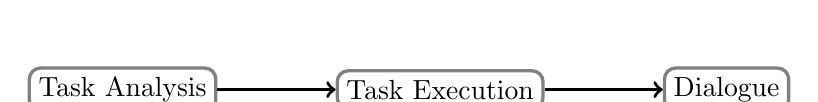
\begin{tikzpicture}
        \node[right] at (0, 0) (task)[rectangle, rounded corners, text centered, draw=gray, very thick] {Task Analysis};
        \draw [very thick, ->] (task.east) -- ++(1.5cm, 0) 
            node[right] (exec)[rectangle, rounded corners, text centered, draw=gray] {Task Execution};
        \draw [very thick, ->] (exec.east) -- ++(1.5cm, 0)
            node[right] (dial)[rectangle, rounded corners, text centered, draw=gray] {Dialogue};
        \end{tikzpicture}
    \caption{Model to identify peer interactions between participants}
    \label{fig:peer-model}
\end{figure}



\subsection{Results}

We identified a total of 142 peer interactions from our user study, categorizing 71 as effective, 35 as ineffective, and 36 as unknown. Study pairs averaged approximately 11 tools recommended between participants within each session. To quantitatively analyze the data collected from the experiment, the Mann-Whitney-Wilcoxon (W) test was used to evaluate ordinal data (\textit{politeness}, \textit{persuasiveness}, and \textit{receptiveness}) and Pearson’s chi-squared ($\chi^2$) test was used to evaluate categorical data (\textit{time pressure} and \textit{tool observability}). All statistical tests were calculated with an alpha level of $\alpha=.05$ and odds ratios (OR) were used to measure effect size.

\begin{figure}
\centering
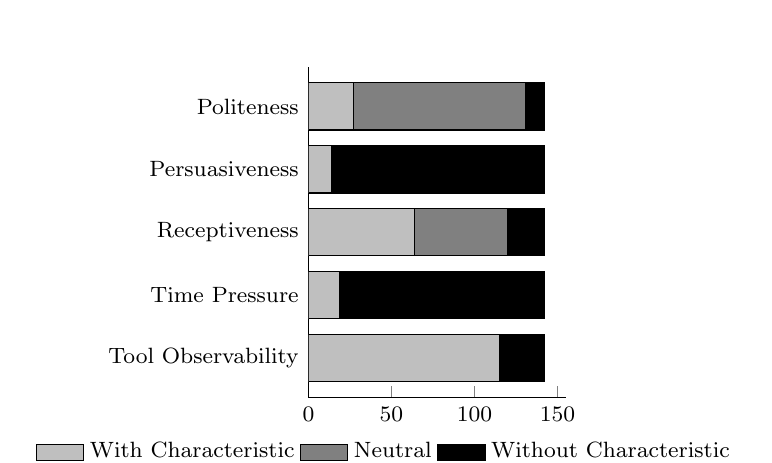
\begin{tikzpicture}
\begin{axis}[
    xbar stacked,
    legend style={
    legend columns=3,
        at={(xticklabel cs:0.3)},
        anchor=north,
        draw=none
    },
    ytick=data,
    axis y line*=none,
    axis x line*=bottom,
    tick label style={font=\footnotesize},
    legend style={font=\footnotesize},
    label style={font=\footnotesize},
    xtick={0,50,100,150},
    width=.4\textwidth,
    bar width=6mm,
    xlabel= Number of Recommendations,
    yticklabels={Tool Observability, Time Pressure, Receptiveness, Persuasiveness, Politeness},
    xmin=0,
    xmax=155,
    area legend,
    y=8mm,
    enlarge y limits={abs=0.625},
]
% With
\addplot[fill=lightgray] coordinates
{(115,0) (19,1) (64,2) (14,3) (27,4)};
% Neutral
\addplot[fill=gray] coordinates
{(0,0) (0,1) (56,2) (0,3) (104,4)};
% Without
\addplot[fill=black] coordinates
{(27,0) (123,1) (22,2) (128,3) (11,4)};
\legend{With Characteristic, Neutral, Without Characteristic}
\end{axis}  
\end{tikzpicture}
\caption{Peer Interaction Characteristic Results}
\label{fig:peer-chars}
\end{figure}

\subsubsection{Characteristics}

Each of the peer interactions observed between participants were categorized based on the peer interaction characteristics and their overall effectiveness. Figure~\ref{fig:peer-chars} displays the number of recommendations that meet each of the characteristics for peer interactions we observed, and Table~\ref{tab:peer-results} displays the effectiveness of recommendations based on the peer interaction 
characteristics.

\begin{table*}[!htbp]
\centering
\caption{Peer Interaction Effectiveness Results}
\resizebox{0.85\textwidth}{!}{%
\begin{tabular}{|l|lll|lll|lll|}
\hline
  \multirow{2}{*}{}  &  \multicolumn{3}{c|}{Effective} & \multicolumn{3}{c|}{Ineffective} & \multicolumn{3}{c|}{Unknown}  \\
\cline{2-10}
 & \textit{n} & & \% & \textit{n} & & \% & \textit{n} & & \% \\
\hline
\multicolumn{8}{|l}{\textit{Politeness}} &  & \\
\hline
Polite & 14 & \posbar{.52} & 52\% & 5 & \posbar{.19} & 19\% & 8 & \posbar{.30} & 30\% \\
Neutral & 52 & \neutralbar{.5} & 50\% & 27 & \neutralbar{.26} & 26\% & 25 & \neutralbar{.24} & 24\% \\
Impolite & 5 & \negbar{.45} & 45\% & 3 & \negbar{.27} & 27\% & 3 & \negbar{.27} & 27\%\\
\hline
\multicolumn{8}{|l}{\textit{Persuasiveness}} &  & \\
\hline
Persuasive & 5 & \posbar{.36} & 36\% & 4 & \posbar{.29} & 29\% & 5 & \posbar{.36} & 36\% \\
Unpersuasive & 66 & \negbar{.52} & 52\% & 31 & \negbar{.24} & 24\% & 31 & \negbar{.24} & 24\%\\
\hline
\multicolumn{8}{|l}{\textit{Receptiveness*}} &  & \\
\hline
Receptive & 39 & \posbar{.61} & 61\% & 9 & \posbar{.14} & 14\% & 16 & \posbar{.25} & 25\% \\
Neutral & 27 & \neutralbar{.48} & 48\% & 14 & \neutralbar{.25} & 25\% & 15 & \neutralbar{.27} & 27\% \\
Unreceptive & 5 & \negbar{.23} & 23\% & 12 & \negbar{.55} & 55\% & 5 & \negbar{.23} & 23\%\\
\hline
\multicolumn{8}{|l}{\textit{Time Pressure}} &  & \\
\hline
Yes & 7 & \posbar{.37} & 37\% & 7 & \posbar{.37} & 37\% & 5 & \posbar{.26} & 26\% \\
No & 64 & \negbar{.52} & 52\% & 28 & \negbar{.23} & 23\% & 31 & \negbar{.25} & 25\%\\
\hline
\multicolumn{8}{|l}{\textit{Tool Observability}} &  & \\
\hline
Observable & 57 & \posbar{.50} & 50\% & 30 & \posbar{.26} & 26\% & 28 & \posbar{.24} & 24\% \\
Non-Observable & 14 & \negbar{.52} & 52\% & 5 & \negbar{.19} & 19\% & 8 & \negbar{.30} & 30\% \\
\hline
\multicolumn{8}{|l}{\textit{Recommendation Type}} &  & \\
\hline
Peer Observation & 16 & \posbar{.30} & 30\% & 5 & \posbar{.09} & 9\% & 32 & \posbar{.60} & 60\% \\
Peer Recommendation & 55 & \negbar{.62} & 62\% & 30 & \negbar{.34} & 34\% & 4 & \negbar{.05} & 5\%\\
\hline
\end{tabular}
}
\label{tab:peer-results}
\end{table*}

\paragraph*{Politeness}

Our analysis shows the majority of participants did not make polite recommendations according to our politeness criteria, classifying 27 tool recommendations between peers as polite, 11 as impolite, and 104 as neutral. Overall, while polite recommendations were more likely to be adopted than impolite ones ($OR = 0.6786$), politeness did not significantly impact the outcome of peer interactions (W, $p = 0.4936$).

\paragraph*{Persuasiveness}

Additionally, we discovered participants were rarely persuasive during peer interactions; there were only 14 persuasive recommendations in total while 128 were unpersuasive  according to our study criteria. While prior work suggests persuasiveness is an important characteristic for convincing users to adopt desired behaviors, this characteristic did not significantly influence the effectiveness of tool recommendations between participants (W, $p = 0.4556$, $OR = 1.4722$).

\paragraph*{Receptiveness}

We found most of the peer interactions in our study incorporated receptiveness, categorizing 64 as receptive, 56 as neutral, and 22 as unreceptive. Overall this characteristic had a high rate of effectiveness, with 61\% of receptive peer interactions leading to the adoption of the recommended tool. Furthermore, we found receptiveness significantly impacts the outcome of tool recommendations between peers (W, $p = 0.0002, OR = 0.2840$). We expand on this finding in the Summary.

\paragraph*{Time Pressure}

Only 19 peer interactions observed between participants were categorized as being under time pressure. Similar to prior work, we found tool recommendations between peers without time pressure were more effective (52\%) and more than twice as likely to be accepted by participants compared to those where time pressure was present ($OR = 2.2857$). However, this characteristic did not play a significant role in the outcome of peer interactions ($\chi^2$, $p = 0.1470$).

\paragraph*{Tool Observability}

Observable tools were far more recommended during peer interactions in our study, with 115 recommendations compared to 27 non-observable tools. However, we found non-observable tool recommendations were slightly more effective (52\%). Examples of observable tools recommended in our study include applications such as R and software features like Sort and pivot tables in Excel. Non-observable tools were primarily keyboard shortcuts. We found that the observability of tools did not significantly impact the effectiveness of recommendations ($\chi^2$, $p = 0.4928$, $OR = 2.4060$).
 
\paragraph*{Peer Interaction Type}

In our analysis, we found that peer recommendations ($n$ = 89) occurred more often than peer observations ($n$ = 53). This indicates software users are more likely to make suggestions for tools and features as opposed to observing a tool and seeking information. Although tools recommended through peer recommendations are more likely to be adopted by users than peer observations (62\%), this difference was not statistically significant ($\chi^2$, $p = 0.3163$, $OR= 0.5729$).

\subsubsection{Summary}

Our results were unable to show that politeness, persuasiveness, time pressure, observability, and interaction type influence tool recommendations between peers. However, we discovered that receptiveness was the only characteristic to significantly impact the outcome of peer interactions. Thus, we conclude no matter how polite, persuasive, time-constrained, or visible a recommendation for a system is, users will not adopt a tool unless they are receptive to using it. The receptiveness characteristic is also the most difficult to implement, since it solely depends on how recommendees receive and respond to suggestions, which recommenders cannot control. Our findings suggest peer interactions are effective because of their ability to foster user receptivity. To define receptiveness, we used criteria from prior work~\cite{Fogg2009Persuasive} that suggests users must demonstrate \textbf{\em desire} and \textbf{\em familiarity} to be receptive to recommendations. We further expound on these criteria in the Discussion.

\section{\TELE}

The \tele is a basic approach for making automated recommendations to software engineers. This technique is referred to as a telemarketer design because behaves similar to a telemarketer that ``calls'' users to deliver static messages, never deviates from the script, and lacks the social context necessary to adjust messages, customize recommendations, or respond to questions and feedback. I developed this technique to define a baseline approach for recommending useful developer behaviors to programmers, such as static analysis tool adoption. With the \tele, a system sends developers a generic message with information about a tool, provides a random example featuring a code snippet incorporating a common programming error irrelevant to the program, and provides the sample output from the tool given this vague error. To evaluate this naive design, I developed a simple bot to identify a baseline for making automated recommendations to software engineers and to better understand how developers respond to recommendations from automated systems.

\subsection{Study Rationale}

While peer interactions are the most effective method of tool discovery, Murphy-Hill and colleagues also discovered they occur infrequently in the workplace~\cite{Murphy-Hill2011PeerInteraction}. Furthermore, Turkle argues technology has become a substitute for face-to-face communications between humans~\cite{turkle2017alone}. Thus, as peer interactions are in decline, it is becoming increasingly important to develop automated systems to recommend developer behaviors. Software engineering research shows bots are useful for automating a variety of programming tasks to improve developer productivity~\cite{storey2016bots}. However, studies also show bots can also be inconvenient and frustrating during interactions with humans~\cite{Hill2015Chatbots, Stanfill86MemBasedReasoning}. To better understand the impact of bots on recommendations to developers, we evaluated the \tele baseline approach in \toolone, an automated system for making development tool recommendations to software engineers on GitHub. In this study, we examined the effectiveness of recommendations from \toolone and gathered feedback from developers who received suggestions from thus system to better understand the impact of automated recommender bots and set the groundwork for designing better solutions in future approaches.


\subsubsection{Research Questions}

In this work, we explored the effectiveness of automated recommendations from bots by using the \tele to discover:

\begin{itemize}[topsep=0pt,itemsep=-1ex,partopsep=1ex,parsep=1ex]
  \item[\textbf{RQ1}] How well do bots encourage developers to adopt useful software engineering practices?
  \item[\textbf{RQ2}] How do developers respond to receiving recommendations from bots?
\end{itemize}

In this evaluation, the goal was to initiate and then identify reactions from developers to evaluate the \tele recommendations in \toolone. The results suggest bots with limited technical knowledge and generic recommendations are ineffective for influencing programmer behavior, and responses from developers provide insight into \toolone was inadequate and implications for improving future systems. This work contributes the \tele, a simple method that provides a baseline for designing automated recommendations, \toolone, a bot that incorporates the \tele to recommend static analysis tools to developers, to motivate the need for new automated recommendation approaches.

\subsection{\toolone: Implementing the \tele} 

To evaluate the \tele, I developed \toolone to generate automated tool recommendations to developers. This bot integrates the \tele by automatically making generic recommendations and adding static analysis tools on repositories using automated pull requests on GitHub. Pull requests are the preferred method to propose changes to GitHub repositories~\cite{PullRequests}, and prior work suggests automated pull requests are useful for upgrading out-of-date dependencies~\cite{Samim2017AutoPullRequests} and fixing static analysis tool violations~\cite{C-3PR}. The initial implementation of \toolone in this evaluation naively recommends \EP, an open source Java static analysis tool,\footnote{\url{http://errorprone.info/}} to developers on GitHub (see Figure~\ref{fig:tool-recommender-bot}a). To automatically integrate \EP into projects, \toolone adds the \EP plugin to repositories that utilize the Maven automation and dependency management tool for Java applications by updating the Project Object Model (\pom) build configuration file to run the tool when the code compiles (Figure~\ref{fig:tool-recommender-bot}b). 

Figure~\ref{fig:sorry-rec} provides a closer look at the automated pull request recommendation text from this system to show how the \tele is implemented in \toolone. First, the recommendation provides generic information about the \EP Java static analysis tool (Fig.~\ref{fig:sorry-rec}.A). Then, the bot also presents a simple example of a Java coding error, using the ``\texttt{==}'' operator to evaluate string equality instead of the \texttt{String.equals()} function (Fig.~\ref{fig:sorry-rec}.B1), and provides the corresponding output from \EP based on the given \texttt{StringEquality} error\footnote{\url{http://errorprone.info/bugpattern/StringEquality}} (Fig.~\ref{fig:sorry-rec}.B2). Ineptly, this simple error may not be present in the program and is irrelevant to the code base of project. An example pull request from our system using the \tele on our repository can be found here\footnote{\url{https://github.com/CSC-326/JSPDemo/pull/2}} and is available in Appendix~\ref{app-sorry}.
% \begin{figure*}[htbp]
% \centering
\begin{figure*}[]
\centering
\subfloat[Pull request recommendation text]{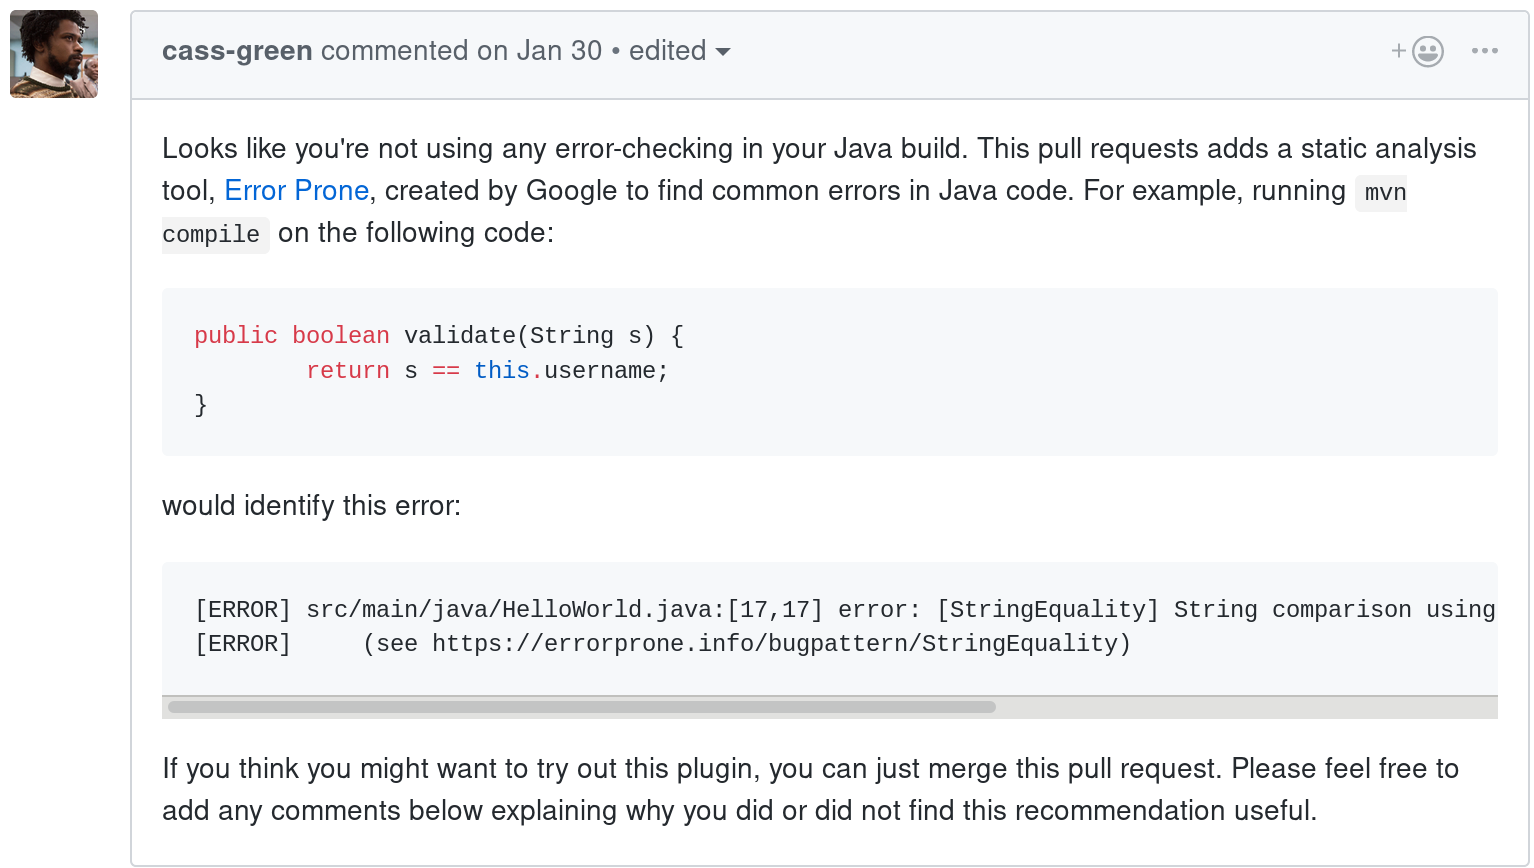
\includegraphics[width=0.45\linewidth]{Chapter-3/images/botse1.png}}
\subfloat[Pull request diff updating a \pom file]{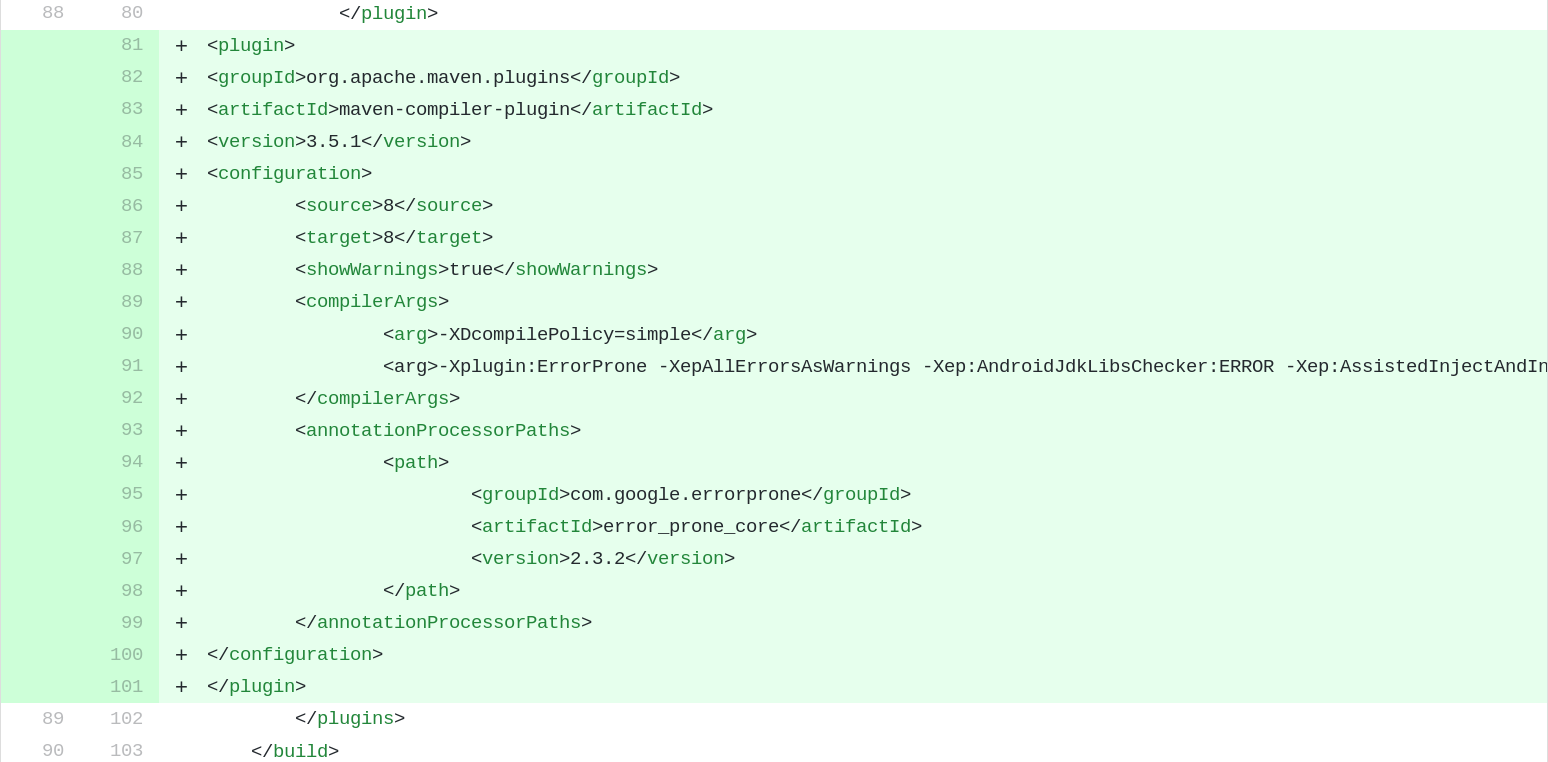
\includegraphics[width=0.5\linewidth]{Chapter-3/images/botse2.png}}
\caption{Example automated pull request from \toolone}
\label{fig:tool-recommender-bot}
\end{figure*}

\begin{figure}[h]
\centering
	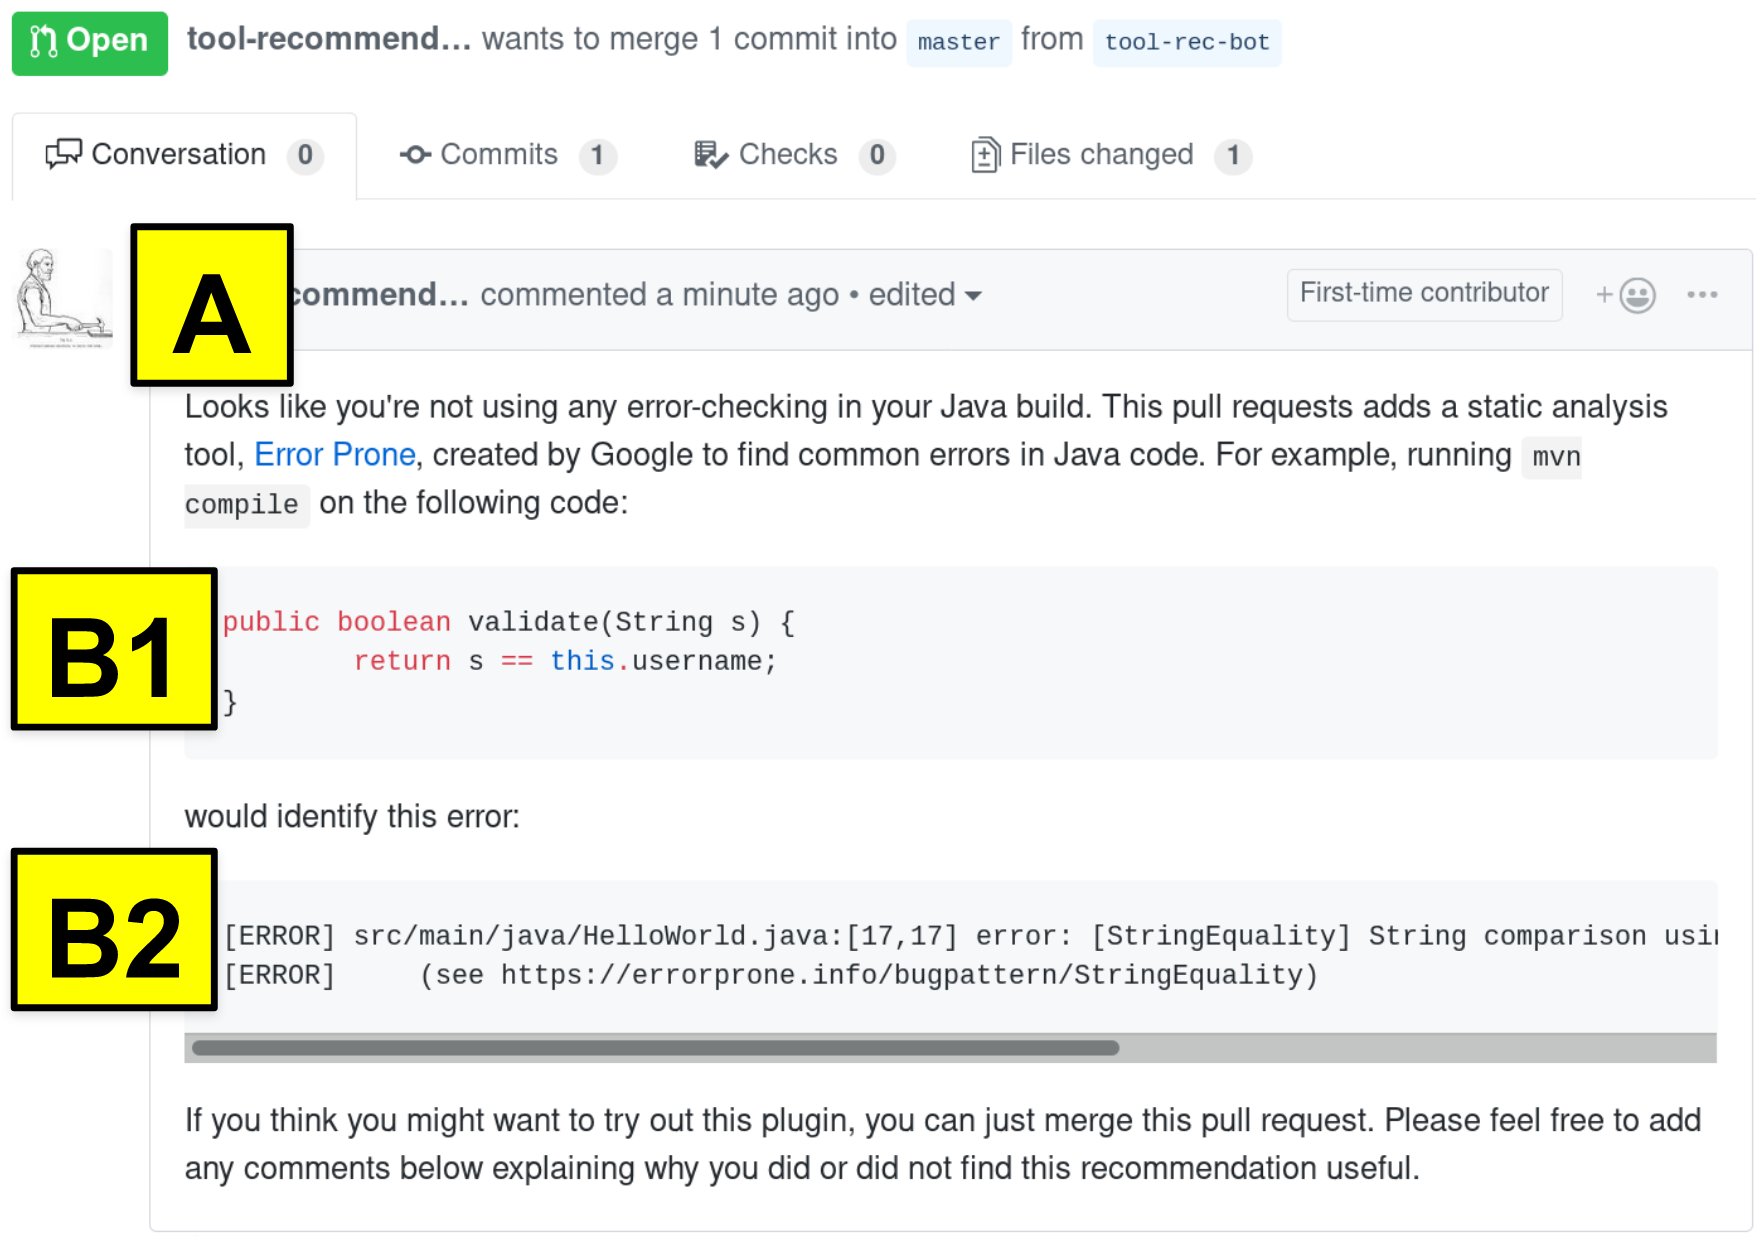
\includegraphics[width=\textwidth]{Chapter-3/images/tool-recommender-bot.png}
	\caption{\TELE recommendation}
	\label{fig:sorry-rec} 
\end{figure}




\subsection{Methodology}

To observe the \tele as a baseline for automated recommendations, I designed a mixed methods study to analyze the effectiveness of \toolone recommendations and collect feedback from developers to further evaluate this simple approach and gain insight into improving future automated recommender systems.

\subsubsection{Data Collection}

\paragraph*{Projects}

To evaluate the baseline \tele approach, \toolone sent automated recommendations to developers working on real-world software applications. The projects used for the evaluation were public open source software repositories on GitHub randomly sampled from the evaluation for Repairnator~\cite{Repairnator}, an automated program repair bot.\footnote{\url{https://github.com/Spirals-Team/repairnator/blob/master/resources/data/results-buildtool.csv}} To be eligible for this experiment, projects selected for the study had to meet the following criteria:

\begin{itemize}[topsep=0pt,itemsep=-1ex,partopsep=1ex,parsep=1ex]
    \item written in Java 8 or higher,
    \item successfully validate and compile with Maven,
    \item do not already include \EP in the build configuration
\end{itemize}

Due to the fact that \EP analyzes Java code, our evaluation was limited to projects written in that programming language. To determine projects that build with Maven, we checked to ensure repositories contained a \pom file in the highest-level directory and confirmed the project could be validated and compiled before adding the tool plugin. We also verified that projects did not already utilize \EP by analyzing \pom files to make sure the \EP plugin was not present to avoid making recommendations to projects that already use the tool and target developers less likely to know about it. Overall, we identified 52 projects that met these criteria to use for this study. The list of GitHub repositories used in the evaluation of the \tele in \toolone is available in Appendix \ref{app-sorry-projects}. These selected projects that received automated pull request recommendations from our bot varied in functionality, programming language, contributions, and size. 

\subsubsection{Determining the effectiveness of \tele recommendations}

To evaluate the \tele, we categorized recommendations as \textit{effective} and \textit{ineffective} based on the status of automated pull requests from \toolone. On GitHub, developers have the option to merge pull requests and incorporate them into the repository\footnote{\url{https://docs.github.com/en/enterprise-server@2.22/github/collaborating-with-issues-and-pull-requests/merging-a-pull-request}} or close pull requests without merging them.\footnote{\url{https://docs.github.com/en/enterprise-server@2.22/github/collaborating-with-issues-and-pull-requests/closing-a-pull-request}}. Additionally, developers can also ignore pull requests by leaving them open. For our evaluation, merged automated pull requests indicated an effective recommendation because developers showed a willingness to try \EP and adopt the recommended tool into their repository by merging the changes from \toolone into their code base. For example, in the pull-based software development model, merged pull requests indicate contributions from external developers are approved to be integrated into the source code for a repository~\cite{gousios2014exploratory}. Alternatively, closed or ignored pull requests implied the recommendation was ineffective. The \tele pull request recommendations were monitored for one week to categorize the recommendations. 

To assess the baseline \tele automated recommendation approach, we calculated the rate of effectiveness was calculated by measuring the percentage of merged pull requests out of the 52 \toolone recommendations sent. Additionally, we aggregated comments from GitHub developers on pull requests to analyze how programmers reacted to receiving a \tele recommendation on their repository. In \toolone automated pull requests, our bot encouraged developers to provide feedback on recommendations by asking developers to ``Please feel free to add any comments below explaining why you did or did not find this recommendation useful''. This qualitative data was compiled and analyzed to determine how developers reacted to receiving \tele recommendations from a bot and collect feedback on this simple approach.

\subsection{Results}

The \toolone system sent 52 automated pull requests recommending \EP to developers on GitHub using the \tele. On these recommendations, we received a total of 24 comments from developers or other automated systems. To analyze the data collected, we calculated the merge rate of pull request recommendations from \toolone and examined feedback from programmers to determine effectiveness.

\begin{table}[h]
\centering
\caption{\toolone Effectiveness Results}
\begin{tabular}{ |c|c|c| } \hline
  & \textit{\textbf{n}} & \textbf{Merge Rate} \\ \hline
 Merged & 2 & 4\% \\ \hline 
 Closed & 10 & 19\% \\ \hline
 No Response & 40 & 77\%\\ \hline 
\end{tabular}
\label{tab:sorry-results}
\end{table}


\subsubsection{Recommendation Effectiveness}

Our findings show that the \tele is not effective for influencing developer behavior (see Table~\ref{tab:sorry-results}). In this evaluation, \toolone was only able to make two successful recommendations out of 52 total notifications (4\%). The remaining automated pull requests, 10 closed and 40 receiving no response from developers, resulted in an overwhelming 96\% of \toolone recommendations categorized as ineffective. Furthermore, while two recommendations from our system were merged, in one case a GitHub issue was created to report problems with the project build based on the changes by \toolone and the pull request was reverted in a later pull request to remove \EP from the project. Even though the tool was eventually removed, we still categorize this instance as an effective recommendation because the developers accepted the pull request and tried the tool before removing it.

\subsubsection{Feedback}

Overall, we observed 24 total pull request comments on 17 unique projects that received recommendations from \toolone. Of the 24 comments, six were made by automated systems on the pull requests to provide information for first-time contributors, request Contributing License Agreement (CLA) signatures, or present code coverage updates. Thus, we received 18 responses from 15 individual developers on 14 recommendations, most of which was negative feedback. Additionally, of the recommendations that received feedback from developers through pull request comments ($n = 14$), 86\% were ineffective and immediately rejected and closed by users ($n = 11$) or left open and never revisited by a developer ($n = 1$). 

While we received some positive reactions from developers on \toolone recommendations, even on those that were not merged (i.e. ``\textit{lgtm, Good Contribution}'' (P9), ``\textit{Thanks for sharing it}''(P13)), the majority of feedback was poor (i.e. ``Please stop using automated tools with a lack of understanding against random repos on github.'' (P6), ``\textit{Automated advertising is spam!}'' (P8)). Overall, the analysis of developer comments posits the main criticisms from developers were about breaking builds ($n = 8$) and messing up the \pom formatting ($n = 5$). We further investigate this feedback to provide themes describing why the \tele in \toolone was ineffective.

\subsection{Summary}

Our results suggest simple bots are ineffective for influencing the behavior of developers. Most \tele recommendations were ineffective, ignored or rejected by developers. This motivates the need for new design approaches and improvements to recommender bots to enhance recommendations and encourage developers to adopt better behaviors. Based on feedback from developers who received naive recommendations from \toolone, we discovered the main drawbacks of the \tele are a lack of \textit{\textbf{social context}} and interrupting \textit{\textbf{developer workflow}}. These concepts are explained and further outlined in the Discussion section.

\section{Discussion: \textit{Developer Recommendation Preconditions}}


Based on the results from these preliminary studies, we uncovered four concepts useful for designing automated behavioral recommendations to developers based on the efficacy of peer interactions and inadequacy of the \tele: \textbf{\em desire}, \textbf{\em familiarity}, \textbf{\em social context}, and \textbf{\em developer workflow}. At a minimum, automated recommender systems must incorporate these \textit{developer recommendation preconditions} in order to make convincing recommendations for software engineers. Below we explore each concept, providing definitions, examples from the completed evaluations, and illustrations from existing software engineering literature.

\subsection{Desire}

Demonstrating desire, or users expressing eagerness to adopt recommended tools and practices, led to effective recommendations between participants in the peer interactions user study. For example, in peer interaction observed during the study participant L12 recommended using the multi-level sorting functionality in Excel. Their partner, L11, demonstrated a desire to use this feature by responding ``\textit{Oh! Add level! Yes, awesome!}'', and the multi-level sorting tool was adopted for completing the rest of the study tasks. Meanwhile, in another session one participant recommended using R for analyzing data to complete a task, but their partner responds ``\textit{No, no, no...}'' (S14). This suggests recommending desirable tools and behaviors can increase adoption among developers, while a lack of desire can negatively impact the outcome of a recommendation. 

Software engineering research also suggests desire impacts the adoption of activities and behavior by developers. For instance, Senyard and colleagues suggest desire is important for motivating programmers to contribute to and maintain successful open source software projects~\cite{senyard2004have}. Furthermore, Murphy-Hill and colleagues found that one barrier to the adoption of useful development tools and practices is \textit{developer inertia}, which refers to when programmers are unwilling to switch from their current workflow and do \textit{not} desire to share or learn about new software engineering tools because they ``feel that they do not need to discover a new tool because existing tools will do the job''~\cite{Murphy-Hill2015HowDoUsers}. Prior work proposes using history-based recommender systems to track user behavior and recommend desirable tools based on their activity~\citep[p.~16]{Murphy-Hill2012Fluency}. To effectively recommend developer behaviors useful for completing programming tasks, recommendations must include desirable and advantageous tools and practices to encourage adoption by developers.

\subsection{Familiarity}

Another takeaway from the peer interactions user study is that users are more likely to adopt recommendations for well-known and recognizable tools and concepts. We observed comments from participants explicitly expressing familiarity and knowledge about recommended tools or their functionality. For instance, in one interaction when L8 recommended using the \texttt{COUNTIF} function in Excel, L7 was familiar with the feature and navigated to the menu to adopt the tool replying ``\textit{Yeah...here we go}''. On the other hand, we found unfamiliar tools negatively impacted recommendations. For example, when a S10 proposed using R to complete a task, their partner responded ``\textit{I don’t know R}'' (S9), and the partner's unfamiliarity with R led to an ineffective recommendation. According to our results, recommending familiar tools can increase the effectiveness of recommendations for developer behavior. This points to a need to incorporate familiar concepts to developers when recommending beneficial development tools and practices.

There are several ways familiarity can impact behavior adoption. For example, familiarity can also lead to \textit{developer inertia}, where programmers prefer familiar tools and processes over of adopting new systems. Prior work also suggests increasing employee knowledge about their workplace and environment, or \textit{work familiarity}, improves their performance~\cite{goodman1992familiarity}. In software engineering, research shows familiarity impacts the completion of tasks and coordination among distributed development teams~\cite{espinosa2002shared}, increasing code comprehension, or familiarity with code, improves development practices~\cite{ko2006exploratory}, and unfamiliarity in the Eclipse\footnote{https://www.eclipse.org/ide/} development environment led to disorientation and decreased productivity~\cite{de2006using}. To incorporate familiarity, prior work propose using history-based systems ranking commands based on similarity using collaborative filtering~\cite{Murphy-Hill2012Fluency}. Additionally, existing recommender systems posit organization-wide learning~\cite{linton2000owl} and collecting user history from networked workstations~\cite{ToolBox} to suggest tools used by colleagues in similar circumstances.

\subsection{Social Context}

The results from the \tele~study show this approach was ineffective because of its lack of social context. This refers to the standard practices and community activities necessary to participate in software engineering by interacting with developers and contributing to projects. Examples of these activities include adhering to formatting and style guidelines, participating in code review discussions, and agreeing to CLAs. The most common complaint we received from GitHub users on \toolone recommendations related to social context was that this system did not follow project style guidelines and disconfigured the whitespace of \pom files when automatically adding the \EP plugin (see Figure~\ref{fig:tool-recommender-bot}b). For example, developers replied ``\textit{The automated tool you use messed up the pom.xml formatting to an extent that I could not see it}'' (P5) and ``\textit{This change removes quite a lot if important things from the POM file}'' (P7), even though \toolone only added the \EP plugin and nothing was removed from configuration files. This suggests our bot's inability to conform to the social context surrounding software development discouraged developers from adopting recommendations.

Social aspects of computing play a major role in making recommendations to developers. For example, prior work argues software engineering is a social activity~\cite{ahmadi2008survey}, peer interactions between colleagues are the most effective mode of tool discovery~\cite{Murphy-Hill2011PeerInteraction}, social media has changed the way developers learn about and share new information~\cite{begel2010social, singer2014twitter}, and social factors influence the adoption of security development tools~\cite{Xiao2014Security}. Furthermore, research shows integrating into social context impacts the effectiveness of automated recommendations. For example, Wessel and colleagues evaluated the usage of bots in open source software and found that problems integrating into social context, specifically limited decision-making abilities and poor communication and feedback, were the biggest challenges developers face during interactions with bots~\cite{wessel2018power}. Prior work also found that systems emulating humans receive better responses from developers and are more effective than recognizable bot accounts~\cite{murgia2016among}. Thus, effectively integrating recommendations into the social context of software engineering can improve the adoption of development practices and tools.

\subsection{Developer Workflow}

The second theme derived from user feedback on \toolone was that the \tele approach disrupted developer workflow, or the existing processes used by programmers to complete development tasks and deliver software. The most notable example of this was the fact that automated pull requests recommendations for \EP often broke continuous integration builds for repositories (see Figure~\ref{fig:error}). However, adding a new static analysis tool to projects often introduced errors and caused the existing infrastructure to fail. Out of the 52 pull requests made, at least 17 resulted in a broken build. Many developers complained about this in their feedback on \toolone, saying the pull requests ``\textit{has introduced erroneous behavior to the build.}'' (P10), ``\textit{Thanks for the contribution, but given the number of errors, I think it would cause more harm than good ;)}'' (P11), and ``\textit{Your change itself looks good, but it seems CI's failing somehow}'' (P12). Furthermore, P5 and P7 were both concerned about the impact on the overall build time. This inability to smoothly integrate into the workflow of developers prevented users from adopting \tele recommendations from \toolone.

Software engineering literature also notes the importance of integration into the workflow of developers. For example, research shows that developers at Google and Facebook primarily ignore static analysis tool warnings that are not integrated into their development workflow~\cite{sadowski2018lessons,Distefano2019Facebook}. Additionally, Johnson and colleagues report the primary reasons software engineers avoid static analysis tools are due to their lack of customizability and poor integration into their existing processes~\cite{Johnson2013Why} while Rahman et al. show that considering the existing workflow of development teams influences software engineers' adoption of continuous integration and build automation tools~\cite{Akond2017BuildTools}. Furthermore, Tonder suggest successful integration of bots with human workflows is important for improving the effectiveness of program repair bots~\cite{Tonder19ProgramRepairBots}. To improve recommendations for developer behaviors, systems should suggest tools without breaking existing development mechanisms and easily integrate into the workflow of developers.

\begin{figure}[H]
\centering
	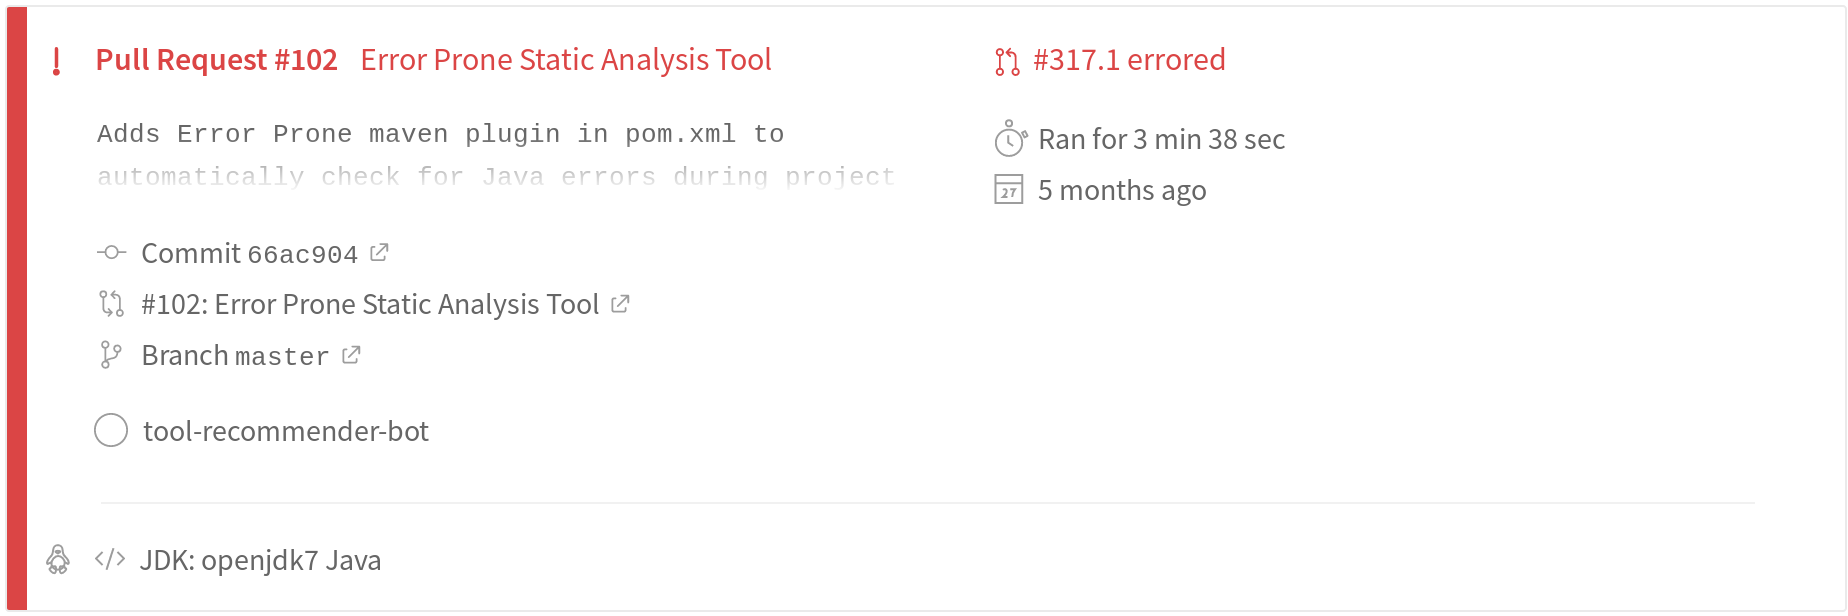
\includegraphics[width=\textwidth]{Chapter-3/images/error.png}
	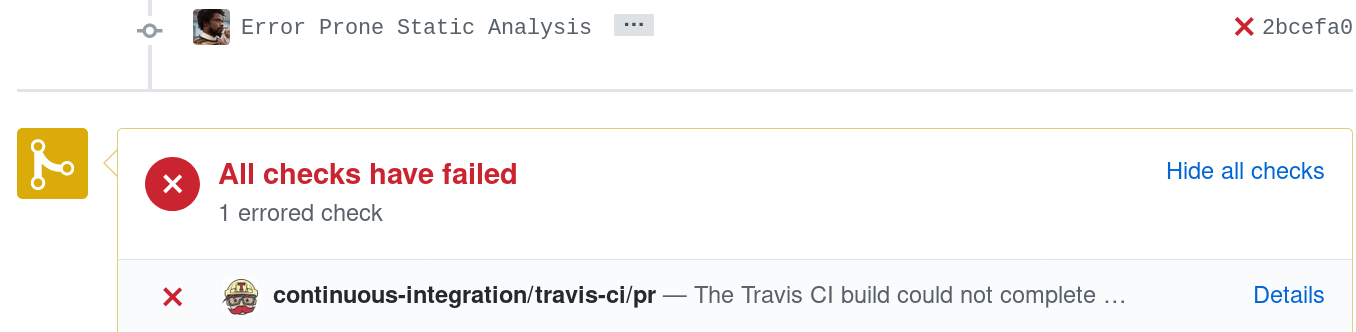
\includegraphics[width=\textwidth]{Chapter-3/images/error2.png}
	\caption{Example of \toolone causing project builds to fail}	
	\label{fig:error} 
\end{figure}

\chapter{Developing the Conceptual Framework}
\label{chap-framework}

The preliminary evaluations investigate what makes effective developer recommendations by exploring the effectiveness of peer interactions and the failures of the \tele. Altogether, these studies posit four \textit{developer recommendation preconditions}, or aspects necessary to make effective recommendations to programmers, \textbf{desire}, \textbf{familiarity}, \textbf{social context}, and \textbf{developer workflow}. However, as opportunities for peer interactions decline and bots produce inadequate suggestions, how can these prerequisites be incorporated into automated recommendations to encourage developer behaviors? This chapter introduces \FRAMEWORK, a state-of-the-art approach to design automated systems by presenting desirable and informative recommendations to developers within their development environment and workflow.


\section{Developer Recommendation Choice Architectures}

Choice architecture refers to the organization of the context in which humans make decisions~\cite{thaler2013choice}. To improve the decision-making of humans, Johnson and colleagues posit 11 practical tools for choice architects, or ``anyone who present(s) people with choices'', valuable for structuring decisions and describing options to encourage the adoption of target behaviors~\cite{johnson2012beyond}. In this work, I view software engineering researchers and toolsmiths are also \textit{choice architects}, creating tools and practices requiring developers to make decisions while developing and maintaining software applications. Thus, I argue the presentation and organization of these decisions to developers impacts the choices they make in their work.

% the developer behavior adoption problem  

To further improve software engineering bots, I introduce \FRAMEWORK, a conceptual framework to design automated recommendations from bots. This approach is motivated by the findings from the preliminary studies (Chapter~\ref{chap-peer}), software engineering literature, and prior work in nudge theory. To devise this framework, I analyzed the tools for choice architecture and apply these concepts in a development context. This mapping, presented in Table~\ref{tab:framework}, derived three principles for designing developer recommendations: \textbf{\em actionability}, \textbf{\em feedback}, and \textbf{\em locality}. By incorporating these concepts into automated notifications, we can improve the way decisions are presented to developers and encourage adoption of useful tools and practices. For the remainder of this chapter, we provide definitions, motivation, and example for each principle and present a formative evaluation of this framework exploring actionable recommendations.

\newgeometry{margin=1in}
\begin{landscape}
\thispagestyle{empty}
\begin{table*}
%/centering
\caption{Developer Recommendation Choice Architectures}
    \begin{tabular}{ |l|l|l| }
	\hline
	\textbf{} & \textbf{Choice Architecture Tool~\cite{johnson2012beyond}} & \textbf{Definition} \\
	\hline
	\multirow{2}{*}{\textbf{\em Actionability}} 
	 & Technology and decision aids & Introducing technology to aid decision makers in choice tasks \\ \cline{2-3}
	 & Use defaults & The way decision makers initially encounter choice tasks \\ \hline
	\multirow{6}{*}{\textbf{\em Feedback}}
	 & Reduce number of alternatives & Limiting the number of choice options presented to decision makers \\ \cline{2-3}
	 & Focus on satisficing & Helping users consider outcomes that lead to higher choice satisfaction \\ \cline{2-3}
	 & Attribute parsimony and labeling & Limiting the number of characteristics presented with options \\ \cline{2-3}
	 & Translate and rescale for better evaluability & Presenting attributes to increase impact and clarity \\ \cline{2-3}
	 & Customized information & Personalization to account for individual differences between decision-makers \\ \cline{2-3}
	 & Focus on experience & Considering the background and knowledge of decision-makers \\ \hline
	\multirow{3}{*}{\textbf{\em Locality}}
	 & Limited time windows & Providing time restrictions for users to make decisions \\ \cline{2-3}
	 & Partitioning of options & Groups or categories of options or attributes \\ \cline{2-3}
	 & Decision staging & Dividing decisions into multiple stages \\ \hline 
\end{tabular}
\label{tab:framework}
\end{table*}
%\vfill
\raisebox{-8.646cm}{\makebox[\linewidth]{\thepage}}
\end{landscape}
\restoregeometry

\subsection{Actionability} 

Actionability refers to the ease with which developers can adopt behaviors presented in recommendations. Nudge theory research suggests actionability is a key concept for encouraging humans to make better decisions. For example, Thaler and Sunstein suggest a simple nudge is to make target behaviors easy to apply because ``many people will take whatever option requires the least effort, or the path of least resistance''~\citep[p.~85]{nudge}. Similarly, Johnson suggests incorporating technology aids and using defaults are actionable ways to influence human behavior. For example, Madrian and Shea implemented the default rule to nudge employees to enroll in retirement plans. By having users automatically opt-in to 401k plans instead of requiring manual signing up, they discovered increased enrollment, with 98\% of new employees selecting a plan within 36 months, and improved money-saving behaviors~\cite{madrian2001power}. 

In the \tele evaluation, we found developers disapproved of recommendations from \toolone because of their deficiencies integrating into development workflows and making more work for developers. For example, P3 commented ``This introduces a bunch of errors, can you check whether they are worth fixing or configure the plugin so as to ignore the false positives?''. Software engineering research also shows actionability is important to developers for adopting development tools and practices. For instance, Heckman and colleagues examined the concept of actionability through static analysis notifications in AAITs (actionable alert identification techniques) to help developers identify and resolve defects~\cite{Heckman11Actionable}. Additionally, Evans and colleagues show that by automatically turning on security analyses in the \textsc{Split} static analysis tool\footnote{\url{https://splint.org/}} increased the amount of security vulnerabilities fixed~\cite{evans2002splint}. We propose actionable development tool and behavior recommendations can increase adoption from developers.

\subsection{Feedback} 

The feedback principle refers to providing clear and relevant information to developers. Sunstein and Thaler note ``the best way to help Humans improve their performance is to provide feedback'' and ``choices can be improved with better and simpler information''~\citep[p.~92,~204]{nudge}. Johnson suggests practical techniques for improving feedback to decision-makers during choices such as limiting the number of options, presenting desirable outcomes, adding labels, reducing the attributes of choices, providing comprehensible content for choosers to evaluate, customizing information and messages, and relating to knowledge and experiences~\cite{johnson2012beyond}. Behavioral science research shows enhanced feedback on decisions improves human behavior. For instance, most people order familiar and repeated meals at fast food restaurants, however nudges such as providing information on the amount of calories in food and customized recommendations for daily caloric intake encouraged consumers to purchase unfamiliar and healthier meals~\cite{Wisdom2010Healthy}.

The results from the peer interactions study suggest providing information about desirable outcomes and targeting familiar concepts of tools and behaviors can incorporate receptiveness into recommendations. Similarly, the \tele study found generic and irrelevant recommendations from \toolone were unproductive, violating social context, and respondents longed for details that ``\textit{would actually help}'' and ``\textit{attach[ing] a report with actual findings in our code instead of just some generic example}'' (P7). Software engineering research also suggests feedback to developers factors in influencing their behavior. For instance, Barik and colleagues examined the structure of compiler error messages on how developers resolved problems~\cite{barik2018should}. Furthermore, Cerezo and colleagues suggest that \textit{user-driven communication} can improve the perception of chatbots compared to bot-driven techniques~\cite{cerezo2019building}. To improve the effectiveness of automated recommendations to software engineers, we believe providing useful information and feedback will improve the likelihood developers adopt useful behaviors.

\subsection{Locality} Locality refers to the setting of recommendations in the context of developers completing programming tasks. Johnson presents several tools for incorporating choice architecture into the setting of choices, including restricting the amount of time for users to make decisions, organizing options into groups, and dividing decisions into multiple states~\cite{johnson2012beyond}. Prior work studying RSSEs also suggests \textit{when} and \textit{what} to recommend are challenges for automated recommender systems~\cite{happel2008challenges}. To describe locality in recommendations for developers, we divide this concept into two subcategories: \textit{spatial} and \textit{temporal} locality.

\subsubsection{Spatial:} Spatial locality refers to the location where developer receive recommendations. Behavioral science research suggests the location of options matters when encouraging humans to adopt beneficial behaviors. For example, Hanks found that by changing the location of vegetables and fruits in a high school cafeteria, they found an increase in the amount of healthier foods purchased and consumed by students~\cite{Hanks2012Lunchroom}. The preliminary studies also suggest location matters in recommendations. For example, in the peer interactions study a participant recommended the Find and Replace functionality in Excel and their partner responds ``\textit{Where's the find and replace?}'' (S12), displaying their unfamiliarity with the feature. 

Software engineering research shows the placement of decisions impacts the behavior of programmers, as developers prefer notifications located in convenient locations. For example, in a collaboration with Smith et al. we developed \textsc{Flower}, an Eclipse code navigation plugin created to help developers avoid disorientation by incorporating \textit{in situ} design principles to prevent users switching between views during code search. We found the location of suggestions within the coding editor of the IDE led to increased efficiency with branchless navigation for developers to find security vulnerabilities and received positive feedback from participants~\cite{Flower}. Thus, I propose automated recommendation systems for encouraging developer behaviors should situate suggestions in convenient and detectable locations to improve the decision-making of software engineers.

\subsubsection{Temporal:} Temporal locality refers to the timing of recommendations made to developers. Nudge theory suggests timing of decisions influences human decision-making. For example, an effective nudge for farmers in Kenya was to change the time of year for fertilizer discounts, and this time-limited window encouraged them to make purchases earlier and improve the harvest of crops~\cite{duflo2011nudging}. In the \tele study, developers mentioned the potential impact of adopting \toolone recommendations on the timing of their project builds led to ineffective recommendations. For example, P7 desired information about ``\textit{the over head in terms of build time}''. These naive recommendations also came at inconvenient times for developers who did not have the bandwidth to fix additional issues and breaking builds, such as one respondent who commented, ``\textit{Can you fix the errors reported by your tool in the build so that I can see the proposed changes?}'' (P17).

Software engineering research also shows that the timing of recommendation within programmers' workflow is important for increasing adoption of developer behaviors. For example, Distefano examined configuring static analysis tools to run at \textit{diff time}, or on code contributions submitted by developers during code review before being merged into the code base, and found that this rescheduling increased the fix rate of reported bugs up to 70\% compared to nearly 0\% for times outside the development workflow, such as assigning bug lists to developers overnight~\cite{Distefano2019Facebook}. Alternatively, untimely recommendations led to programmers ignoring code navigation strategies from Spyglass~\cite{viriyakattiyaporn2009challenges}. To improve the effectiveness of automated recommendations, systems should make timely suggestions to programmers within their workflow to increase their desire to adopt useful software engineering behaviors and practices.



\section{Preliminary Evaluation}

To explore the impact of \framework on the behavior and decision-making of software engineers, I conducted a preliminary evaluation to provide an overview of actionable recommendations. While this work focuses solely on \textit{actionability}, the subsequent studies and future work aim to study all of the conceptual framework principles.

\subsection{Methodology}

To evaluate actionability in automated recommendations, this study incorporates multiple methods of analyzing survey responses to quantitatively evaluate developer preferences and qualitatively collect feedback on actionable recommendations.

\subsubsection{Data Collection}

\paragraph*{Participants}

Professional software engineers were recruited to participate in this study. Overall, we received responses from 15 software developers and participants had an average of 7.3 years of industry programming experience. 

\paragraph*{Study Recommendation}

For this evaluation, we presented participants with recommendations to fix a \texttt{PEP 3105} Python 3 style warnings. This warning indicates Python \texttt{print} statements are are now \texttt{print()} functions in the latest version of the programming language.\footnote{\url{https://www.python.org/dev/peps/pep-3105/}} For instance, line 9 of Listing~\ref{listing:pep} contains an example \PEP violation. This simple recommendation also has larger implications for improving the behavior of developers because, as of January 1, 2020, Python 2 is officially no longer supported. The programming language announced there will be ``no new bug reports, fixes, or changes'' to the older version and encouraged developers to upgrade to Python 3.\footnote{\url{https://www.python.org/doc/sunset-python-2/}} Our sample recommendations proposed fixing \PEP warnings and upgrading the code base to Python 3.

\paragraph*{Survey}

To investigate the impact of actionability in automated suggestions, we presented participants with sample automated recommendations to fix \PEP warnings and upgrade to the latest version of Python. The survey presented participants with screenshots of two suggestions, one actionable and one static, and asked participants to select which recommendation they preferred and provide reasoning behind their choice. Additionally, we asked participants to input their years of professional development experience and to provide general feedback on designing automated recommendations from bots. The survey distributed to developers is available to view in Appendix~\ref{app-sorry2-survey}.

\begin{listing}
\centering
 \caption{Example of a \PEP static analysis violation and fix}{}
\begin{minted}[xleftmargin=6cm,fontsize=\small,linenos,firstnumber=9]{python}
if status is True:
-   print 'passed'
+   print('passed')
\end{minted}
\label{listing:pep}
\end{listing}


\subsubsection{Determining the effectiveness of actionable recommendations}

In this formative evaluation, we surveyed developers to investigate actionability in automated recommendations. The survey included actionable and static recommendations to fix \PEP errors and a message encouraging users to upgrade from Python 2 to Python 3. The static recommendation presented to participants is displayed in Figure~\ref{fig:sorry2-static}, while Figure~\ref{fig:sorry2-action} presents the actionable recommendation. Based on the \framework design principles, both of these recommendations incorporate the same \textit{feedback} (information to promote repairing the \PEP error, proposing a fix, and encouraging users to upgrade to Python 3), \textit{spatial locality} (placed on Line 10 of a sample code snippet containing a \PEP error), and \textit{temporal locality} (located on an open pull request before the code is merged). 

\begin{figure}[H]
\centering
	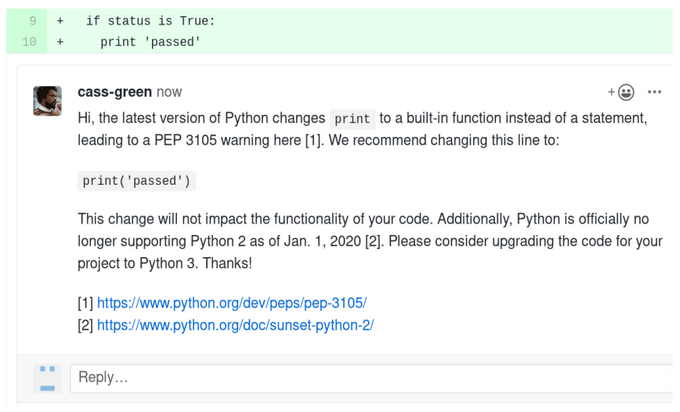
\includegraphics[width=0.8\textwidth]{Chapter-4/images/static.png}
	\caption{Static recommendation to fix a \PEP error}
	\label{fig:sorry2-static} 
\end{figure}

\begin{figure}[H]
\centering
	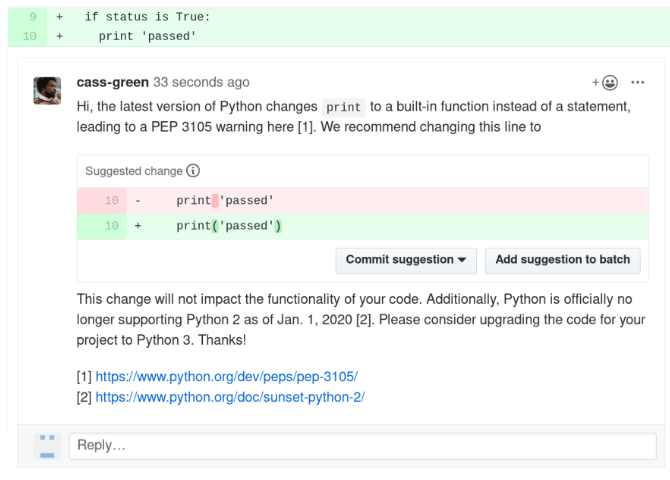
\includegraphics[width=0.8\textwidth]{Chapter-4/images/actionable.png}
	\caption{Actionable recommendation to fix a \PEP error}
	\label{fig:sorry2-action} 
\end{figure}

\newpage
However, these sample notifications differ on the \textit{actionability} of recommendations. The static recommendation would require developers to re-submit a pull request to make the proposed change (\texttt{print('passed')}). On the other hand, the actionable recommendation incorporates a ``Commit suggestion'' button which allows developers to automatically commit the suggested fix for the \PEP violation to their code. This technology aid makes the decision of whether or not to fix the error simpler for developers by providing a solution and incorporating the ability to easily integrate the suggested code changes into their workflow and code. We aim to discover how this design decision impacts developers' preferences for adopting behaviors from automated recommendations.

\subsection{Results}

Our survey responses, presented in Table~\ref{tab:results}, reveal 100\% of developers ($n = 15$) preferred the actionable recommendation over the static approach. This indicates developers are much more likely to adopt recommendations that make it easier to adopt suggestions. Developers also provided feedback praising the actionable recommendation, reporting it ``\textit{lets you automatically merge it}'' (P8), ``\textit{appl[ies] the change automatically}'' (P3), ``\textit{provide[s] an actionable short cut}'' (P2), and ``\textit{can directly commit the change instead of having to do a manual commit}'' (P10). Thus, we conclude that actionability is an effective approach for encouraging developers to improve their behavior. 

\begin{table}[htbp]
    \centering
    \caption{Survey Results on the Actionability of Recommendations}
    \begin{tabular}{|c|c|c|} \hline
          & \textbf{\em n} & \textbf{Percent}\\ \hline
         static & 0 & 0\% \\ \hline
         actionable & 15 & 100\% \\ \hline
    \end{tabular}
    \label{tab:results}
\end{table}

\section{Discussion}

To improve developer decision-making, I present \framework, a conceptual framework which incorporates concepts from nudge theory to design actionable, informative, and convenient automated recommendations. This approach, motivated by the preliminary studies exploring effective developer recommendations as well as prior work in behavioral science and software engineering, posits \textit{actionability}, \textit{feedback}, and spatial and temporal \textit{locality} as key factors influencing the adoption of developer behaviors. As choice architects, software engineering researchers and bot developers can enhance the way decisions are presented to programmers by integrating this framework into automated recommendation systems. To evaluate this approach, I conducted a formative evaluation investigating the impact of actionability on developers' perception of automated recommendations, and found participants significantly prefer actionable notifications in contrast to static ones. By incorporating this framework into automated recommendations, the thesis of this dissertation argues that systems can encourage the adoption of behaviors useful for improving code quality and productivity of developers (Chapter~\ref{chap-thesis}). The next two chapters present further evaluations of \framework by analyzing existing recommender systems (Chapter~\ref{chap-suggs}) and introducing new tools incorporating this framework (Chapter~\ref{chap-bot}) to analyze its impact on the decision-making and behavior of developers.


\chapter{Analyzing Existing Recommendation Systems}
\label{chap-suggs}

\Framework is a framework to create automated recommendations improving how developers perceive and respond to suggestions by incorporating \textbf{\em actionability}, \textbf{\em feedback}, and \textbf{\em locality}. The preliminary evaluation of this framework shows developers prefer actionable recommendations, however each principle factors into recommendations to developers and their overall impact on developer behavior remains unknown. To evaluate this approach, I first analyze the framework within existing recommender systems. This chapter explains how \suggs adheres to the \framework principles and presents two studies analyzing \sugg to explore their impact on the style and impact of recommendations. Additional study materials for these evaluations are available in Appendix~\ref{app-suggs}.

\section{GitHub \textit{Suggested Changes}}
\label{sec-suggs}

GitHub, a popular online code hosting site with millions of developers and billions of code contributions each year~\cite{Octoverse}, introduced the \textsl{suggested changes} feature as a public beta release in October 2018. Since the announcement, the GitHub blog reports users have been ``quick to adopt suggested changes'' into their code review processes with over 100,000 uses within weeks of the initial public beta release, accounting for 4\% of pull request comments and 10\% of code reviewers during that time~\cite{SuggestedChanges2}. This system, illustrated in Figure~\ref{fig:suggs}a-c, allows developers to make recommendations for code improvements to peers on GitHub during pull request reviews. The work presented in this chapter is the first research, to my knowledge, to study the \suggs feature.

To use the \suggs feature, a reviewer observes a deficient line of code on a pull request, they can click on the plus (+) sign on the line of code in question, in this case Line 9, to generate a pull request review comment (Figure~\ref{fig:suggs}a). Then, a text box is displayed for reviewers to enter a comment and they can click the \suggs icon (
\includegraphics[height=1em]{Chapter-5/images/sugg_icon.png}) to propose changes to the line of code. Figure \ref{fig:suggs}b presents an example recommendation, where the reviewer encourages the developer not to use a single character variable name, which is discouraged in the Java programming language for non-temporary variables,\footnote{\url{https://www.oracle.com/java/technologies/javase/codeconventions-namingconventions.html}}, and recommends changing the variable name from \texttt{int c} to a more descriptive identifier \texttt{int count}. Once the reviewer finishes their suggestion, they can click on the ``Start a review'' button to submit their recommendation. Finally, the developer who submitted the pull request can see the suggested change on their code, shown in Figure \ref{fig:suggs}c, and has the ability to commit, edit, or ignore the proposed modification. Clicking on ``Commit changes'' provides the ability to automatically incorporate the proposed change into the pull request as a new commit.

\suggs can also be considered a nudge, encouraging developers to improve their code without providing incentives to apply reviewer suggestions (i.e. money) and allowing alternative changes to improve the code (i.e. \texttt{int compute}). Additionally, this system incorporates all of the developer recommendation choice architectures presented in Chapter~\ref{chap-framework}: it is \textit{actionable} by providing the ability for developers to automatically apply recommendations from peers by clicking on a button to commit suggestions (Figure~\ref{fig:suggs}c); provides informative \textit{feedback} to users by providing a specific improvement to the code with an optional comment (Figure~\ref{fig:suggs}b); has convenient \textit{locality} with recommendations appearing to developers on the exact line of code within their pull request and during code reviews before contributions are merged into the code (Figure~\ref{fig:suggs}a). By evaluating the design of this novel feature, I aim to explore the impact of \framework on recommendations to developers within this system and provide implications for designing of future recommender bots.

\begin{figure*}[htbp]
\centering
\subfloat[New suggested changes feature on GitHub pull requests]{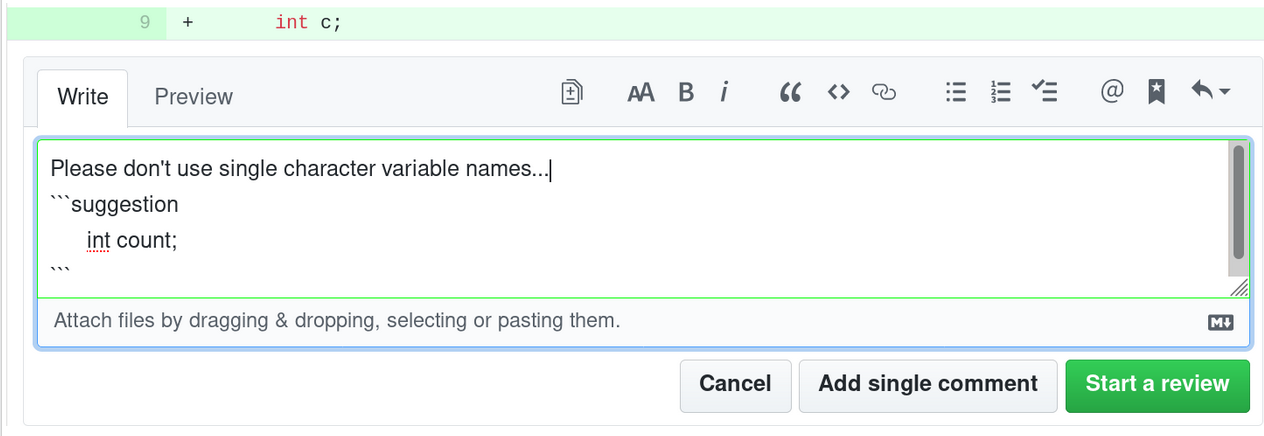
\includegraphics[width=0.9\linewidth]{Chapter-5/images/sugg1.png}}\\
\centering
\subfloat[Reviewer adds comment and suggested change to modified line of code~]{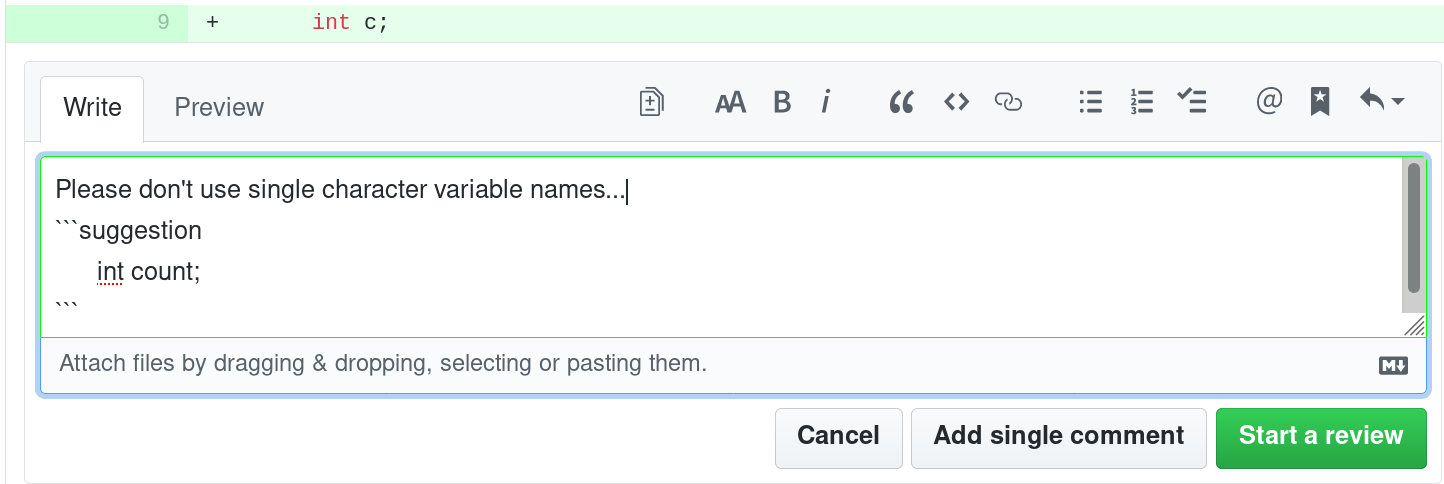
\includegraphics[width=0.9\linewidth]{Chapter-5/images/sugg2.png}}\\
\subfloat[Developer can apply suggested change and commit to PR]{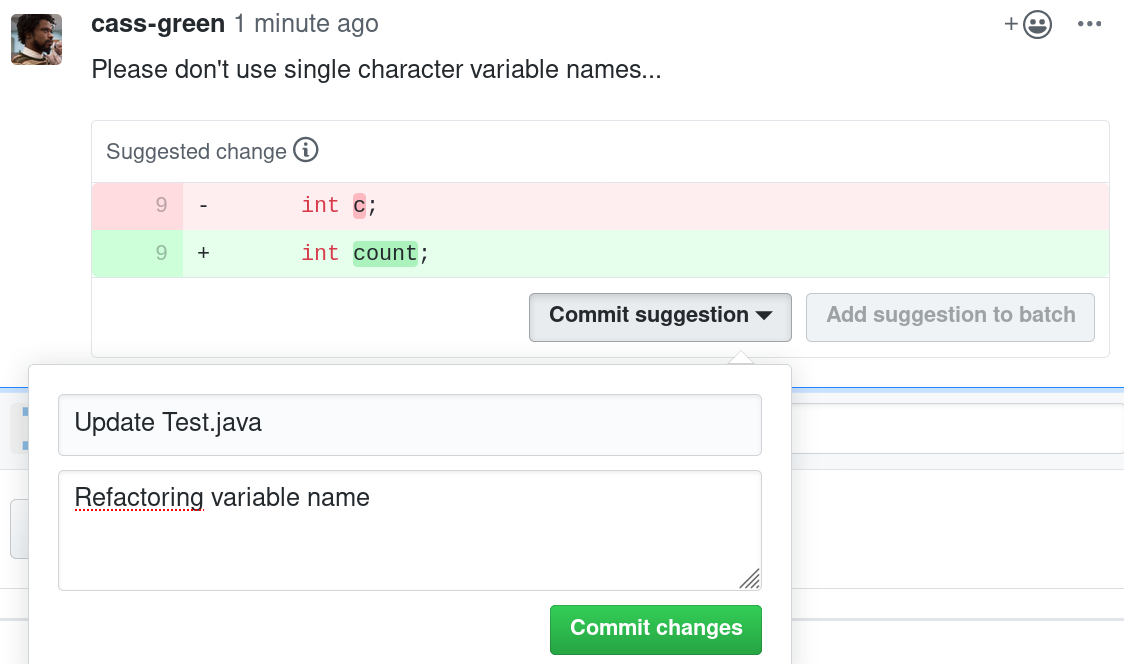
\includegraphics[width=0.9\linewidth]{Chapter-5/images/sugg3.png}}
\caption{Example of the \suggs feature}
\label{fig:suggs}
\end{figure*}



\section{Recommendation Styles}

\textit{Recommendation styles} refers to techniques utilized by automated approaches for conveying developer behavior recommendations to programmers. Prior work suggests styles of suggestions can impact the decision-making and behavior of users. For example, Fischer argues active help systems that automatically provide help to users are more effective than passive approaches~\cite{Fischer1984ActiveHelpSystems}. Additionally, software engineering researchers have proposed a wide variety of recommendation tools and techniques to encourage developers to adopt useful practices with diverse manners of presenting information to users, such as badges~\cite{trockman2018badges}, Twitter~\cite{singer2014twitter}, software documentation~\cite{Forward2002Documentation}, live-coding~\cite{blackwell2014collaboration}, crowd-sourcing~\cite{gordon2015codepourri}, gamification~\cite{barik2016game}, idea gardening~\cite{cao2012ideagarden}, and Testing on the Toilet~\cite{Murphy-Hill2019Toilet}.

\subsection{Study Rationale}

To overcome decreasing opportunities for human-to-human recommendations and the increase of distributed development teams, researchers have explored creating recommender systems for software engineering to support programmer decision-making and improve the behavior of developers~\cite{RSSE}. However, studies such as ~\cite{Hill2015Chatbots}, and~\cite{viriyakattiyaporn2009challenges} show that developers often find automated recommendations from systems ineffective. Additionally, the results of the \tele study found that the simple recommendation approach in \toolone failed because of its lack of social context and intrusiveness into development workflows. This work seeks to evaluate several system-to-human recommendation approaches, including the popular \suggs feature, to discover their impact on the presentation of suggestions to programmers and gain insights into improving future automated recommendation approaches.


\subsubsection{Research Question}

To discover the impact of \suggs as a recommendation system for automated recommendations, we sought to answer the following research question:

\begin{itemize}
    \item[\textbf{RQ}] How well does the suggested changes feature generalize to different styles of recommendations?
\end{itemize}

To answer this research question, I devised a user study that consisted of professional software engineers evaluating static analysis tool recommendations from four different systems: \suggs, emails, GitHub issues, and GitHub pull requests. We analyzed these systems to evaluate the design of these features for making recommendations to software engineers. The results show that programmers preferred tool recommendations using \sugg due to its content and design. The goal of this study is to discover the impact of this feature, and hence the \framework framework, on sharing information to developers and to provide implications for improving recommendations to software engineers. This study contributes a user study exploring different recommendation styles and a mock-up design for a future automated recommender system incorporating \suggs.

\subsection{Styles}

To analyze the recommendation style of \suggs, this work compares mock automated static analysis tool recommendations from this system to similar notifications given via emails, issues, and pull requests. Little is known about \sugg and their impact on recommendations to developers, however the comparative systems examined in this evaluation were selected based on prior work exploring them as a mechanism for recommendations and their influence in software engineering. Additionally, I provide a breakdown of how each recommendation system analyzed during this study fit within \framework in Table~\ref{tab:framework} (to see how \suggs support the framework, see Section~\ref{sec-suggs}).

\textit{Email.} Email is one of the most popular forms of communication today, with approximately 4 billion users sending and receiving over 293 billion emails daily~\cite{EmailIsNotDead}. Additionally, Sterne and colleagues suggest emails are the most powerful tool to reach audiences and spread information in marketing~\cite{sterne2000email}. Emails are also prevalent in software engineering, where prior work shows communication with emails in distributed agile development teams differs from face-to-face and instant messaging communication~\cite{Niinimaki2011EmailAgile} and proposes using emails to deliver security tool recommendations to developers~\cite{Jordan2014Designing}. Furthermore, many systems, such as the Coverity static analysis tool\footnote{\url{https://scan.coverity.com/}} and GitHub security scans,\footnote{\url{https://docs.github.com/en/github/administering-a-repository/managing-security-and-analysis-settings-for-your-repository}} alert developers and provide reports via email.

However, emails generally do not fit into the \framework framework for designing recommendations for software engineers. For example, email systems usually have poor actionability and lack the ability for users to automatically apply suggestions made in recommendations. Additionally, this system has very poor locality, with email recommendations often presented in a separate location in an application outside of developers' programming environments and they can be received at any time during the software development process. These problems can lead to a variety of problems for workers, including email overload~\cite{Dabbish2006EmailOverload} and reduced productivity from interruptions~\cite{jackson2001cost}. Despite the shortcomings of email for actionability and locality, this system is able to provide clear and comprehensible feedback in suggestions to users depending on the content of the message text.

\textit{Issues.} The GitHub issue tracker is a useful system for tracking a variety of information for repositories on GitHub~\cite{Issues}. For example, more that 20 million issues were closed by developers in 2019~\cite{Octoverse}. Additionally, issues are another method for developers to make and receive recommendations on GitHub. Bissyandé and colleagues found that the majority of issues are labeled as ``bugs'', but argue those labeled as ``feature'' or ``enhancement'' that recommend improvements and new functionality to projects are ``equally important for issue reporters''~\cite{bissyande2013issues}. Prior work has also observed issues to find correlations between issues and enhancements added to projects~\cite{krishna2018connection} and analyzed issue labels to visualize activity in open source software repositories~\cite{izquierdo2015gila}.

GitHub issues have several characteristics that comply with \framework principles. For example, this system can provide understandable recommendations to developers in the title, description, or comments of issues. It can also provide further feedback with features such as labels to categorize the issue, milestones to group issues within the context of the project, and assignees to specify developers to complete the task.\footnote{\url{https://guides.github.com/features/issues/}} For spatial locality, while issues do not occur within the code itself but they are present on the same project repository in a separate section. However, like emails, GitHub issues are not actionable, due to the fact developers cannot automatically implement recommendations from this system, and have poor temporal locality in that issues can be submitted to GitHub projects at any time during the development process. Research also shows GitHub issues can frequently go unnoticed or ignored by developers~\cite{sorbo2019wontfix}.

\textit{Pull Requests.} Pull requests provide a mechanism for developers to propose changes to projects on GitHub~\cite{PullRequests}. We examined pull requests because they are the most popular method to recommend code changes to repositories. For example, in 2019 there were over 200 million pull requests submitted and 87 million merged into code repositories across the platform~\cite{Octoverse}. Research suggests pull requests are also useful for making suggestions to developers on GitHub. For example, Padhye and colleagues show recommending enhancements to projects is the most common purpose for pull requests submitted and merged into repositories~\cite{padhye2014contributions}. Additionally, prior work has explored generating automated pull requests to encourage developers to update package dependencies~\cite{Samim2017AutoPullRequests}, fix static analysis errors~\cite{C-3PR}, and recommend static analysis tools~\cite{Sorry}.

GitHub pull requests closely adhere to the \framework framework principles. Developers are able to automatically merge proposed changes from pull requests into their source code, making it an actionable system. However, recommendations made to developers through review comments are not actionable and require users to manually apply suggestions. Pull requests can incorporate feedback by providing coherent suggestions to developers through the description of pull requests and the repository changes proposed to projects. Recommendations from this system also have high spatial locality, being submitted on the same GitHub repository with the ability to be integrated directly into the code base. Additionally, development teams usually have code review processes that provide a workflow for developers to inspect changes proposed in pull requests.\footnote{https://docs.github.com/en/github/collaborating-with-issues-and-pull-requests/about-pull-request-reviews} However, similar to issues and emails the timing of pull requests cannot be controlled by project maintainers, which means they can occur on repositories at any time during the development process. This may also factor in to pull request evaluation latency, or the amount of time for developers to address pull requests on repositories~\cite{yu2015wait}, and contribute to reviewers' difficulty prioritizing contributions~\cite{gousios2015work}.

\begin{table}[H]
\centering
\caption{Mapping recommendation styles to \framework}
\begin{tabular}{ |c|c|c|c|c| } \hline
  & \textit{\textbf{Actionability}} & \textit{\textbf{Feedback}} & \textit{\textbf{Spatial Locality}} & \textit{\textbf{Temporal Locality}}\\ \hline 
 Emails & \Circle & \CIRCLE & \Circle & \Circle \\ \hline 
 Issues & \Circle & \CIRCLE & \RIGHTcircle & \Circle \\ \hline 
 Pull Requests & \RIGHTcircle & \CIRCLE & \CIRCLE & \RIGHTcircle \\ \hline 
 Suggested Changes & \CIRCLE & \CIRCLE & \CIRCLE & \CIRCLE \\ \hline 
\end{tabular}
\label{tab:framework}
\begin{tablenotes}
\CIRCLE Incorporates principle \RIGHTcircle Somewhat incorporates principle \Circle Does not incorporate principle
\end{tablenotes} 
\end{table}

\subsection{Methodology}

To compare recommendation styles, I developed a user study using a mixed methods approach to collect quantitative and qualitative data from developers participating in an interactive think aloud study examining static analysis tool recommendations.

\begin{table}[h]
\centering
\caption{Recommendation Styles Study Participants}
\resizebox{\textwidth}{!}{
\begin{tabular}{ lllll } \hline
  \textbf{Participant} & \textbf{Experience (years)} & \textbf{GitHub Familiarity} & \textbf{OSS Contribution Frequency} & \textbf{Tool Usage Frequency} \\ \hline
 P1 & 30 & Very Familiar & Occasionally & Very Frequently \\  
 P2 & Less than 1 & Moderately Familiar & Never & Never \\ 
 P3 & Less than 1 & Very Familiar & Rarely & Moderately Frequent \\  
 P4 & 8 & Very Familiar & Very Frequently & Very Frequently \\ 
 P5 & 10 & Familiar & Rarely & Moderately Frequent \\
 P6 & 5 & Moderately Familiar & Occasionally & Very Frequently \\
 P7 & 6 & Familiar & Frequently & Very Frequently \\
 P8 & 6 & Familiar & Very Frequently & Very Frequently \\
 P9 & Less than 1 & Moderately Familiar & Occasionally & Very Frequently \\
 P10 & 1 & Moderately Familiar & Occasionally & Very Frequently \\
 P11 & 3 & Familiar & Very Frequently & Very Frequently \\
 P12 & 3 & Familiar & Rarely & Very Frequently \\
 P13 & 1 & Moderately Familiar & Never & Never \\
 P14 & 1 & Moderately Familiar & Never & Frequently \\
 \hline
 
\end{tabular}}
\label{tab:style-participants}
\end{table}
\begin{figure}[!htbp]
\centering
	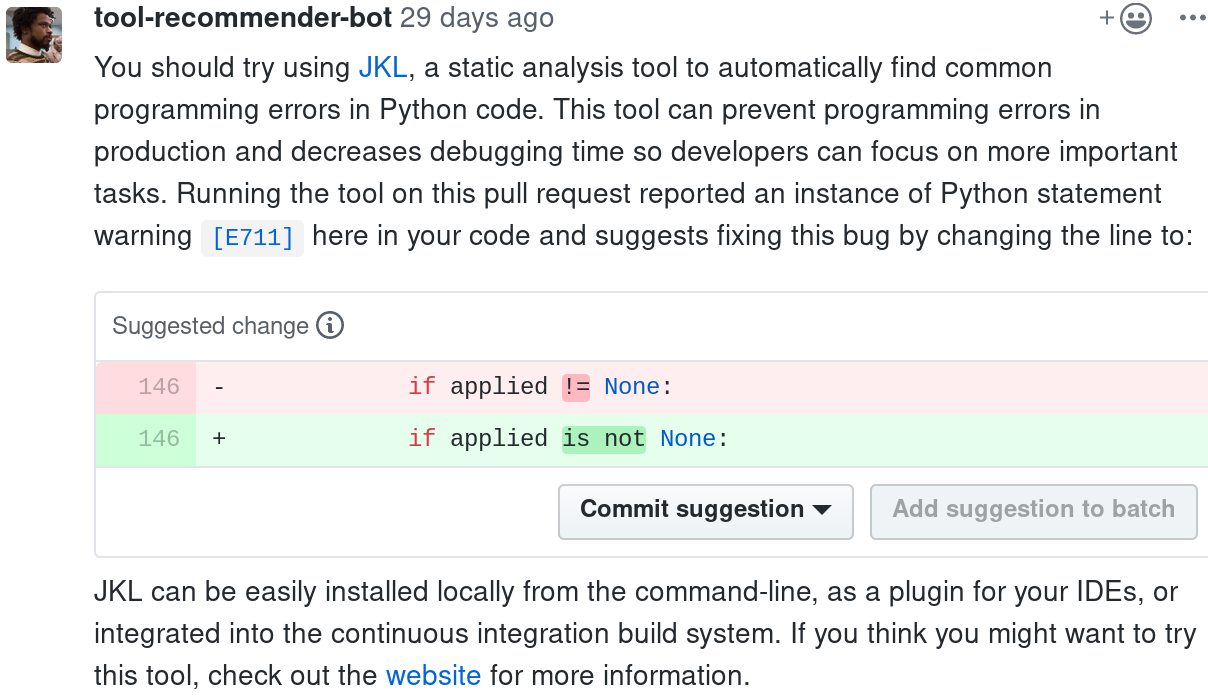
\includegraphics[width=0.9\textwidth]{Chapter-5/images/sugg-recommendation.png}
	\caption{Example of the \suggs recommendation style}	
	\label{fig:suggestion-rec} 
\end{figure}


\subsubsection{Data Collection}

\paragraph*{Participants}

We recruited 14 professional software developers, presented in Table~\ref{tab:style-participants}, to participate in this study. Participants averaged 5 years of industry experience and consisted of workers from various companies spanning many different positions such as Software Engineer, Quality Engineer, Consultant, Data Migration Consultant, Support Specialist, User Researcher, and Technical Test Lead. All of participants were at least moderately familiar with GitHub and most had experience contributing to open source projects and incorporating development tools into their work.

\paragraph*{Study Design}

To collect data to answer the research question, we conducted a user study examining \suggs, issues, pull requests, and emails as systems for static analysis tool recommendations. The study tasks involved these types of recommendations because static analysis tool adoption is a developer behavior that is beneficial for software development teams, however prior work shows developers often avoid these systems in practice~\cite{Johnson2013Why}. During the study, each participant evaluated recommendations from all four systems simulated in an experimental GitHub repository they were not familiar with. Participants were asked to interact with each recommendation system, as if they received it as an automated notification for their own project, and to use think-aloud methods~\cite{jaspers2004thinkaloud} to verbalize their thoughts as they explored each system. Then, to conclude the study we conducted semi-structured interviews to gather feedback from participants on each recommendation style and general opinions about tool recommendations.

\subsubsection{Determining the impact of recommendation styles}

To explore the impact of recommendation styles on developer behavior, participants interacted with tool recommendations from emails, issues, pull requests, and \sugg. A sample \suggs recommendation used for this study is available in Figure~\ref{fig:suggestion-rec}, while examples from the other systems are available in Appendix~\ref{app-suggs-recs}. Recommendations from each system contained similar text recommending a static analysis tool that finds and prevents programming errors to participants, however suggestions differed in the presentation of recommendations according to each system. For example, \suggs incorporates all of the \framework principles (Section 6.1) while emails have poor \textit{actionability} to adopt recommendations and unfavorable \textit{locality} outside of the development environment and workflow. To avoid bias, tools were recommended with made-up names (\texttt{ABC}, \texttt{DEF}, \texttt{GHI}, and \texttt{JKL}) and varying programming languages (JavaScript, Java, and Python) to prevent participants from relying on their previous experience with existing tools and programming languages. The order participants interacted with each system was also randomized to prevent order bias in our results. 

Each study session was screen and audio recorded, and the semi-structured interview responses were transcribed to analyze developers' interactions with the systems. During the interview, the moderator asked participants to provide a five point Likert-scale rating on how likely they would adopt the tool recommended from each system. A score of four or five indicated participants were likely to accept the suggestion while a one or two indicated they were unlikely to adopt the tool and would reject the recommendation. Additionally, we asked subjects to discuss what they liked and disliked about each approach and to provide general observations on automated recommendations. Two researchers performed an \textit{open card sort}~\cite{begel2014analyze} to extract themes from open-ended responses and provide insight for improving recommendation systems to developers. The raters individually grouped statements based on responses concerning effective and ineffective recommendations, then came together to analyze and discuss the derived themes and sort the data accordingly.

\subsection{Results}

To analyze the data collected from our user study, we averaged Likert scale ratings and used the Kruskal-Wallis statistical test to calculate the likelihood of adoption and measure developer preferences. We also present the themes derived from the open card sort providing feedback on each system and general comments on developer recommendations.

\subsubsection{Likelihood of Adoption}

The findings from the user study show that \suggs were the preferred tool recommendation system by participants. Table~\ref{tab:styles-results} presents the average and median Likert scores representing participants' reported likelihood they would adopt the tool recommendation from each method.  The \sugg feature had the highest score averaging a 4 in the 5-point Likert scale ranking for all participants. Additionally, this system had the highest rate of participants likely to adopt the tool presented in the recommendation (85\%), and it was the only method that did not receive a 1 score. We also found that participants' preference for tool recommendations with \suggs was statistically significant ($H$ = 16.7527, \textit{p} = .00079, $\alpha$ = .05) compared to the other systems. This indicates the style of \sugg is preferred by software engineers for receiving recommendations, and this tool has the style of an effective system for improving developer behaviors, such as increasing static analysis tool adoption.

\begin{table}[H]
\centering
\caption{Survey Results on the Likelihood of Recommendation Style Adoption}
\begin{tabular}{ |c|c|c| } \hline
  & \textit{\textbf{Average Score}} & \textit{\textbf{Median}} \\ \hline
 Suggestions & 4 & 4 \\ \hline 
 Pull Requests & 3.71 & 4 \\ \hline 
 Issues & 2.86 & 3 \\ \hline 
 Email & 2.36 & 2 \\ \hline 
\end{tabular}
\label{tab:styles-results}
\end{table}

\subsubsection{Qualitative Feedback}

During the user study, we collected qualitative data through think aloud and a semi-structured interview to learn what developers liked and disliked about each system and gain insight into designing automated recommendation systems. Here, we present comments from participants on each of the different suggestion mechanisms and provide the themes derived from the open card sort on general recommendations.

\paragraph*{Emails}

The majority of participants were unlikely to adopt static analysis tool recommendations via email, ranking this system as a 1 or 2 ($n = 11$). Most developers also provided unfavorable feedback on receiving email recommendations, such as ``\textit{I hate emails}'' (P3), ``\textit{if this came across unsolicited I would feel sort of intruded upon}'' (P4), ``\textit{would honestly be pretty suspicious when I get any email asking to install software on my computer}'' (P12), ``\textit{if I see an email about something it actually gives me less of a view of it}'' (P6), and ``\textit{I'd immediately delete it...I wouldn't even give it a look. I'd actually probably not like that tool even more just because their sending out spam emails}''. However, while most participants disliked tool recommendations sent by email, three participants, P2, P6, and P11, responded they were likely to adopt tools recommended through this system noting ``\textit{it feels personal}'' (P2) and ``\textit{I like email more}'' (P11).

\paragraph*{Issues}

Participants were noncommittal on their likelihood to adopt static analysis tool recommended through GitHub issues, with most participants ($n = 9$) scoring them as a 3. The primary feedback provided from developers on this system was the amount of effort required to learn more information and integrate the tool. For example, P1 noted ``\textit{I'd be much less likely to integrate it [the tool]...that's a lot of work}'', P4 stated ``\textit{I see this as a big time sync to go through and evaluate how many of those actually are issues and how many are false positive things}'', and P14 desired more specific information adding ``\textit{it reads a little more spammy without a code example...It seems like you could just post this message on any project. Why is this useful for my project specifically? I have no idea}''. Additionally, P13 complained about the amount of text within the issue recommendation commenting ``\textit{this one is a ton of words}''.

\paragraph*{Pull Requests}

Developers reported being likely to adopt static analysis recommendations from pull requests on GitHub ($n = 9$). Participants appreciated the timing and location of recommendations from this system on repositories. For example, P7 stated ``\textit{I'd be significantly more likely to try it if I already have a pull request that has all the changes I need to get the tool or something going in the project}'' and P4 added ``\textit{getting pretty quickly an explanation, the actual issue in the code, and you know a basically free way to incorporate that into the process as well as you know the tool itself}''. Alternatively, participants criticized the lack of information provided about tools provided in pull request suggestions, saying ``\textit{it doesn't really outline the steps}'' (P13). P8 and P14 also criticized using pull requests on GitHub as a recommendation system, outside the intended purpose of this feature, stating pull requests should ``\textit{solve a problem rather than tell people they should try to use this thing}'' and ``\textit{it's not that they really want to do a pull request. It's not that their going to be adding to the project...I don't know why it's a pull request specifically}''.

\paragraph*{Suggested Changes}

Our results show participants were significantly more likely to adopt static analysis tool recommendations from \sugg than from emails, issues, or pull requests. Overall 12 developers responded they were likely to accept the recommendation, providing a variety of reasons why they favored \sugg recommendations. Participants praised the location of the recommendation (``\textit{having it comment right here, `This fixes your bug!' That's nice}'' (P8)), the visual aids of the feature (``\textit{this one is definitely better because it's more visual}'' (P13)), and the content of the information provided (``\textit{it has a little more detail}'' (P9) and ``\textit{this has very good detail, very detailed change of the code and so it's clear}'' (P10)). Only one participant (P6) was unlikely to adopt the tool recommended with this feature, stating ``\textit{putting a tool recommendation in a comment of a pull request, it's kind of to me out of place}''.

\paragraph*{General Feedback}

In addition to collecting feedback from developers on each recommendation system, we asked participants to provide general insight into designing effective recommendation systems. The open card sort derived five themes for what developers seek in recommendations. Below we present the categories uncovered in our qualitative analysis and provide representative quotes from participants: \\

\textbf{Examples:} Developers in our study noted examples are important to include in recommendations to support decisions on the adoption of tools. For example, participants specifically mentioned wanting to observe tool usage and output, view demos, and test systems in a local environment. Additionally, respondents desired the ability to easily find and access examples of tools in the documentation and/or on it's website.

\begin{quote}
\textit{``In general I think showing an example of the type of error that it would find, cause that immediately shows some value, I think that helps a lot''} (P4)
\end{quote}

\textbf{Integration:} Participants indicated information about how well tools integrate into their existing processes should be incorporated into recommendations. Workflow details such as how easy it is to install the system, how well it works with other tools (i.e. continuous integration build systems), the impact on resources (i.e. memory, GPU, lagging, etc.), how relevant it is to their project and development needs, and if it adheres to company policies are important details for developers to consider when deciding to adopt tools from automated recommendations.

\begin{quote}
\textit{``I want something that I can install it and use it as quickly as possible with as minimal fussing with it and setup as possible.''} (P5)
\end{quote}

\textbf{Marketing:} Several participants remarked recommendations with text similar to advertising or marketing notifications would deter them from adopting tools from automated suggestions. For instance, developers in our study were suspicious and distrustful of static analysis tool suggestions from emails and unsolicited messages, but were more open to recommendations with human-like communication.

\begin{quote}
\textit{``I'm not sure how the bot would generate the text to do the recommendation but try to make it seem a little more human? Rather than it was written by someone in an advertising agency or something.''} (P7)
\end{quote}

\textbf{Popularity:} Participants reported providing information about the popularity of recommended systems into suggestions is valuable for helping programmers to decide whether or not to adopt development tools. Specifically, developers mentioned seeking information about the usage and reputation of tools from online reviews, meetup groups, colleagues, conference talks, social media, and other resources before incorporating systems into their workflow.

\begin{quote}
    \textit{``Try to highlight the popularity, popularity is so crucial...I care about the adoption. The current adoption, that’s a testimony of the strength''} (P13)
\end{quote}

\textbf{Reliability:} Developers noted information about the reliability of tools and their sources is useful for determining whether or not to adopt them. For instance, study participants mentioned reliable tool output, little to no false positives, predictable behavior, up-to-date documentation, and ongoing development on the tool itself impact their decision-making.

\begin{quote}
    \textit{``[It] definitely needs to work reliably. Any time a tool starts doing things like it occasionally has problems that’s something that makes me want to stop using it...I want the tool to be more reliable than that.''} (P8)
\end{quote}

\subsection{Summary}

Our results show that \suggs are an effective system improving the developer behavior. We found 14 professional software engineers were significantly more likely to adopt automated static analysis tool recommendations from this feature over suggestions from emails, GitHub issues, and pull requests. Further analysis of responses from developers derived themes for improving automated recommendations to improve the behavior software engineers. To provide implications for improving future recommender systems, we combine these themes into two overarching categories for designing effective automated suggestions: recommendation \textbf{\em content} (\textit{Integration}, \textit{Popularity}, and \textit{Reliability}) and \textbf{\em design} (\textit{Examples} and \textit{Marketing}). In the discussion, I present how these categories align with \framework and contribute to the preference for the \suggs recommendations.

\section{Developer Impact}

While the recommendation styles study shows users prefer to receive recommendations from systems incorporating \framework, their \textit{developer impact}, or influence on programming practices, is still unexplored. For example, prior work suggests bots are useful for automating programming tasks and supporting software development activities such as completing continuous integration tasks, running tests, and decreasing code review time and effort in open source software projects~\cite{wessel2018power}. However, our prior work shows that \tele recommendations from \toolone negatively impacted development practices by breaking continuous integration project builds, aimlessly introducing static analysis errors to projects, and violating project style guidelines~\cite{Sorry}. To evaluate the impact of the conceptual framework on development practices, I conducted an empirical evaluation of the \sugg feature to analyze its influence on programming activities and its usefulness for developers on GitHub. 


\subsection{Study Rationale}

The GitHub platform has a variety of methods for developers to make recommendations to each other, such as issues which are useful for recommending new functionality and enhancements to projects~\cite{bissyande2013issues}. GitHub recently introduced the \sugg feature, a novel recommendation system on the platform that allows developers to provide specific and actionable feedback to peers during reviews (see Figures \ref{fig:suggs}a-c)~\cite{SuggestedChanges}. While this feature is increasing in popularity and usage on GitHub~\cite{SuggestedChanges2}, little is known about how developers use \sugg to make recommendations to each other and its impact on development practices. Researchers have performed in-depth analyses on a variety of GitHub features to explore their impact on developer behavior and software engineering practices, including pull requests~\cite{gousios2015work}, issues~\cite{bissyande2013issues}, issue tracker labels~\cite{cabot2015exploring}, links between issues and pull requests~\cite{li2018issue}, repository forks~\cite{jiang2017and}, commit comments~\cite{guzman2014sentiment}, README files~\cite{prana2019categorizing}, stars~\cite{borges2018stars}, and badges~\cite{trockman2018badges}. This study adds to this work by offering an empirical analysis of \suggs to examine their impact on development processes and provide implications for improving future recommender systems.

\subsubsection{Research Questions}

To explore the impact of \sugg on development practices, we investigated the following research questions:

\begin{itemize}[topsep=0pt,itemsep=-1ex,partopsep=1ex,parsep=1ex]
    \item[\textbf{RQ1}] What types of recommendations do developers make with suggested changes?
    \item[\textbf{RQ2}] How effective are recommendation systems on pull requests?
    \item[\textbf{RQ3}] What impact do suggested changes have on pull requests?
    \item[\textbf{RQ4}] How useful are suggested changes for recommendations between developers?
\end{itemize}

To answer these questions, I contrived a multi-methodological study divided into two phases. The first phase seeks to answer the first three research questions by mining GitHub repositories and empirically analyzing the \sugg feature to categorize types of suggestions, measure the effectiveness of this system, and observe its impact on the pull-based software development model. The second phase explores the final research question by collecting qualitative data from developers to provide feedback on their experiences with the \suggs system. The results show \sugg are effective for recommending a variety of changes to programmers and supports developers in the code review process by helping them make suggestions and decisions on proposed changes quicker. Users also find this feature useful because it allows clear communication and easy integration. The main contribution of this work is the first study to empirically analyze the \suggs feature.

\subsection{Phase 1: \textit{An Empirical Study on GitHub Suggested Changes}}

The first phase of this evaluation mines public GitHub repositories to explore the usage, effectiveness, and impact of \sugg.

\subsubsection{Data Collection}

\paragraph*{Identifying suggested changes}

To automatically detect \suggs on pull requests, I developed a script to programmatically parsed pull request review comments to find instances of the \suggtag tag in a review (see Figure~\ref{fig:suggs}b) since this feature is currently not supported by the GitHub API.\footnote{\url{https://github.community/t5/GitHub-API-Development-and/Accessing-the-new-quot-GitHub-Suggestions-quot-via-API-public/td-p/13922}}. This markdown snippet indicates a recommendation was made from a review to a developer on a pull request using this system. The script utilized the PyGithub API\footnote{\url{https://pygithub.readthedocs.io/en/latest/}} to collect repositories for identifying \sugg in on updated pull requests and parsed comments to collect instances of the \suggs feature. To limit our data collected, we only observed activity on pull requests after October 2018 when the \sugg feature was first introduced on GitHub. For categorizing \sugg, we randomly sampled the most recently updated repositories to compile a list of current pull request comments incorporating this feature. To determine the effectiveness of \sugg and their impact on development practices, we analyzed the top-forked repositories on GitHub with pull requests using this feature. For the first research question, we randomly sampled 100 \sugg on the most recently updated pull requests. To answer RQ2 and RQ3, we analyzed a total of 51,250 pull requests, 17,712 \sugg, and over 152,030 pull request review comments on the most forked repositories.

% PyGithub provides an API to retrieve pull request review comments and, similar to our suggested changes detection technique, we searched for instances of the code fence to determine if comments contain code snippets. Overall, we analyzed 152,030 pull request review comments and found 17,712 suggested changes on 51,250 pull requests.

\subsubsection{Categorizing suggested changes}

To categorize \suggs, two researchers performed an \textit{open} coding qualitative analysis on a sample of suggestions. We analyzed instances of this feature on the most recently updated repositories to characterize types of changes developers recommend. The raters independently analyzed \sugg to inspect the code change recommended, the review comment text, and the entire discussion on pull requests to identify categories of changes proposed to peers by developers with this feature. Then, we came together to discuss our derived categories and come to an agreement. Finally, we used our defined categories to classify 100 randomly sampled instances of pull request comments containing the \suggtag tag (inter-rater agreement = 71\%, Cohen's $\kappa$ = 0.5942). The list of sampled \sugg, derived from projects varying in size, programming language, number of contributions, and other repository metrics, are available in Appendix~\ref{app-suggs-sample}. Our main source of discrepancies arose from determining the functionality of suggested changes and deciding if suggestions were correcting or improving lines of code.

\subsubsection{Determining the effectiveness of suggested changes}

To investigate the effectiveness of suggestions, we analyzed \suggs and pull request review comments, two mechanisms for providing recommendations to developers on code contributions. Pull request review comments differ from general pull request and issue discussion comments because they are situated on exact lines of code during the review process. Furthermore, reviewers can suggest specific changes to developers in pull request review comments by using code fences (\fence) to start and end the proposed block of code. For example, Figure~\ref{fig:review-comment} presents an instance of a review comment providing the same recommendation to change \texttt{int c} to \texttt{int count} as the \textsl{suggested change} in Figure~\ref{fig:suggs}c. 

\suggs are a special instance of pull request review comment, allowing reviewers to provide feedback on contributions from developers. The primary difference between \sugg and review comments is the user interface, which involves the ``Commit suggestion'' button to automatically apply recommended changes to pull requests and the highlighted \textit{diff} format to display suggested code modifications in the newer system. To evaluate the effectiveness of code recommendations on pull requests, we compare and contrast both of these features to analyze how they impact recommendations between developers during reviews. To measure effectiveness, the evaluation observed the \textit{acceptance} and \textit{timing} of recommendations from these systems. We further divide these criteria into subcategories: \textit{contribution acceptance} and \textit{recommendation acceptance}, and \textit{contribution time}, \textit{recommendation time}, and \textit{recommendation acceptance time}.

\begin{figure}[b]
\centering
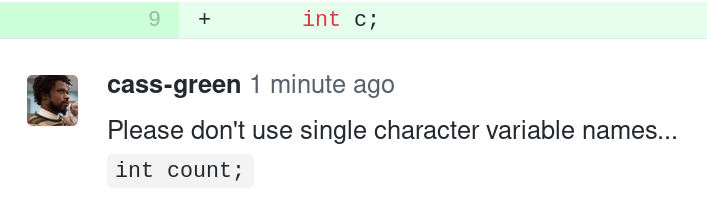
\includegraphics[width=0.6\textwidth]{Chapter-5/images/review_comment.png}
\caption{Example pull request review comment with code}
\label{fig:review-comment}
\end{figure}

\paragraph*{Acceptance}

Acceptance refers to users incorporating proposed changes from another developer. \textit{Contribution acceptance} involves how frequently proposed changes from developers are incorporated into projects. Prior work suggests accepted contributions from developers are a valuable metric for measuring the success and performance of software on GitHub~\cite{mcdonald2013performance} and is necessary for the development, maintenance, and evolution of open source software~\cite{Middleton2018Contributions}. We use this metric to evaluate the adequacy of recommendation systems on pull requests. To study the impact of the recommendations on contribution acceptance, we calculated the merge rate of pull requests containing a code suggestion, either \sugg or pull request review comments with fenced code, and compared it to pull requests without code recommendations. % Contribution acceptance is calculated using \textit{merge rate}, or the percentage of merged pull requests.

\textit{Recommendation acceptance} refers to how often suggestions from each system are approved by developers. The percentage of \sugg and fenced code review comments incorporated into pull requests from our dataset was used to investigate recommendation acceptance. To identify instances of each system, we developed a script to analyze pull request review comments and search for occurrences of \suggtag to identify \sugg and \fence to identify review comments with code. The recommended code within the tags was automatically extracted from the comment. Then, we programmatically checked whether the recommendation was accepted by determining if the extracted code existed in subsequent changes to the pull request by analyzing additional commits to the file after the recommendation was made. If so, we consider the suggestion accepted by the developer. This process was implemented to compare the recommendation acceptance for pull request review comments with fenced code and \sugg.

\paragraph*{Time}

This metric examines the impact of pull request recommendation systems on the overall development process. \textit{Contribution time} refers to the lifespan of pull requests submitted by developers. Prior work outlines factors that influence pull request evaluation latency, or the amount of time to review pull requests on GitHub~\cite{yu2015wait} and analyzes factors that influence merge time of pull requests~\cite{gousios2014exploratory}. Furthermore, research shows the longer it takes to repair issues in code the more expensive and difficult they are to fix~\cite{Williams2007FaultFixTime}. Here, we aim to determine if the presence of code suggestions from review comments or \sugg impacts amount of time to make decisions about contributions from developers. The difference between time of a pull request being opened until when it is merged into the repository by a project maintainer was used to measure contribution time.

\textit{Recommendation time} evaluates the amount of time for developers to make recommendations to peers with a given pull request recommendation system. To analyze the impact of \sugg and pull request review comments with fenced code on development time, we compared how quickly developers compose comments making recommendations with with code on pull requests. This was measured by calculating the amount of time from the creation of a pull request until a reviewer adds a code suggestion with the \suggtag or \fence tags and comparing this recommendation time between each system.

Similarly, \textit{recommendation acceptance time} refers how long it takes developers to accept recommendations with \sugg and review comments with fenced code from reviewers on pull requests. To assess this, we measured the amount of time between a reviewer commenting on a pull request using the \suggtag or \fence tags until the time of a subsequent commit containing the extracted code between the fences. This data was used to compare the effectiveness of \suggs and pull request review comments with code as mechanisms for receiving recommendations from peers on pull requests.

\subsubsection{Evaluating the impact of suggested changes}

To analyze \sugg on development practices, we explored the impact of this system on the pull-based software development model, a popular programming methodology for distributed development teams on code hosting websites like GitHub~\cite{gousios2014exploratory}. Each year millions of pull requests are contributed by developers and merged into repositories on GitHub~\cite{Octoverse}, excluding other online development collaboration platforms such as GitLab\footnote{\url{https://about.gitlab.com/}} and BitBucket.\footnote{\url{https://bitbucket.org/}} Pull requests are the primary method for developers to contribute to projects~\cite{gousios2015work}, and thus a mechanism through which developers provide recommendations to each other virtually. For instance, pull request review comments and \sugg allow users to provide feedback and make recommendations on code contributions to developers. To further evaluate \suggs, we analyzed metrics from existing literature to explore the effect of this feature on pull request timing, coding activity, and collaboration.

\paragraph*{Pull Request Characteristics} 

Prior work posits a variety of metrics derived from the \textit{pullReqs} dataset to explore the pull-based software development model~\cite{gousios2014dataset}. This dataset, consisting of roughly 350,000 pull requests on 900 GitHub repositories, provides a variety of characteristics to describe GitHub pull requests and quantify their impact on the pull-based development model. To explore the impact of \suggs on development practices on GitHub, we calculated the following metrics to analyze pull requests with and without this feature: 

\begin{itemize}[topsep=0pt,itemsep=-1ex,partopsep=1ex,parsep=1ex]
    \item \textbf{\em lifetime\_minutes}: Number of minutes between pull request opening and closing (if closed)
    \item \textbf{\em mergetime\_minutes}: Number of minutes between pull request opening and merging (if merged)
    \item \textbf{\em num\_commits}: Total number of commits for a pull request
    \item \textbf{\em src\_churn:} Total number of lines changed
    % \item \textbf{\em test\_churn:} Total number of test lines changed
    \item \textbf{\em files\_changed:} Total number of files touched by pull request
    \item \textbf{\em num\_commit\_comments:} Number of review comments
    \item \textbf{\em num\_issue\_comments:} Number of discussion comments
    \item \textbf{\em num\_participants:} Number of discussion participants
\end{itemize}


These characteristics were selected to describe the impact of \sugg on development processes and better understand how this feature influences contributor and reviewer behavior on pull requests. To determine the impact of \suggs, we analyzed \textbf{\em lifetime\_minutes} and \textbf{\em mergetime\_minutes} to determine their impact on development time, \textbf{\em num\_commits}, \textbf{\em src\_churn}, and \textbf{\em files\_changed} to analyze their affect on developer productivity, and \textbf{\em num\_commit\_comments}, \textbf{\em num\_issue\_comments}, and \textbf{\em num\_participants} to observe their impact on collaboration between developers. We amassed these metrics and compare these characteristics for pull requests with \suggs and those without this feature.

\begin{table*}[tbhp]
\centering
\caption{Developer Impact Study Data}
\begin{tabularx}{\textwidth}{ lrrrr } \hline
  \textbf{Project} (\textit{Primary Language}) & \textbf{SCs} & \textbf{RCs (w/ code)} & \textbf{PRs} \\ \hline
 qmk/qmk\_firmware (\textit{C}) & 8525 & 9127 (675) & 3600 \\
 nodejs/node (\textit{JavaScript}) & 2252 & 14364 (818) & 5889 \\
 rust-lang/rust (\textit{Rust}) & 2615 & 24139 (1068) & 8475 \\
 go-gitea/gitea (\textit{Go}) & 1317 & 6604 (338) & 2822 \\
 rapid7/metasploit-framework (\textit{Ruby}) & 754 & 4057 (517) & 1252 \\
 Qiskit/qiskit-terra (\textit{Python}) &  626 & 3505 (204) & 1735 \\
 kubernetes/kuberbetes (\textit{Go}) & 556 & 52297 (2645) & 12106 \\
 qgis/QGIS (\textit{C++}) & 481 & 2893 (37) & 2548 \\
 neovim/neovim (\textit{Vim script}) & 208 & 3087 (163) & 1746 \\
 python-pillow/Pillow (\textit{Python}) & 156 & 354 (19) & 650 \\
 mono/mono (\textit{C\#}) & 134 & 6043 (182) & 5821 \\
 lydiahallie/javascript-questions (\textit{Markdown}) & 49 & 43 (2) & 231 \\
 jpmorganchase/quorum (\textit{Go}) & 10 & 192 (13) & 193 \\ 
 firebase/quickstart-android (\textit{Java}) & 5 & 89 (6) & 155 \\
 mavlink/qgroundcontrol (\textit{C++}) & 5 & 261 (14) & 863 \\
 qbittorrent/qBittorrent (\textit{C++}) & 5 & 3966 (205) & 486 \\
 ironhack-labs/lab-advance-querying-mongo (\textit{Markdown}) & 4 & 159 (12) & 753 \\
 kenwoodjw/python\_interview\_question (\textit{Markdown}) & 3 & 2 (0) & 38 \\
 lballabio/QuantLib (\textit{C++}) & 3 & 57 (4) & 146 \\ 
 Azure/azure-quickstart-templates (\textit{PowerShell}) & 2 & 2718 (2) & 1630 \\
 h5bp/Front-end-Developer-Interview-Questions (\textit{HTML}) & 1 & 81 (2) & 56 \\
 qunitjs/qunit (\textit{JavaScript}) & 1 & 77 (11) & 55 \\
 \hline
 \textbf{Total:} & 17,712 & 134,318 (6,937) &  51,250 \\ \hline

\end{tabularx}
\begin{tablenotes}
\centering
\textbf{SCs:} GitHub \textsl{Suggested Changes}~~\textbf{RCs:} Pull Request Review Comments~~\textbf{PRs:} Pull Requests
\end{tablenotes}
\label{tab:sugg-projects}
\end{table*}


\subsection{Phase 2: \textit{Developer Feedback on Suggested Changes}}

The second phase of this study explores the usefulness of \suggs by collecting feedback from developers.

\subsubsection{Data Collection}

\paragraph*{Participants}

To collect feedback from developers, we recruited users who interacted with \suggs. Surveys were emailed to users with publicly available email addresses who either received \sugg on their pull request or made a suggestion on a developer's pull request within six months of the time of this study. Surveys were sent to a total of 580 GitHub users who interacted with the \suggs feature, and we received responses from 43 developers (7.4\% response rate). Throughout the remainder of this chapter, the \see- prefix is used describe \textit{suggestees}, or contributors who received a \textsl{suggested change} on their pull request, and the \ser- prefix indicates a \textit{suggester}, or a reviewer who made a comment with \sugg on a pull request. 


\subsubsection{Determining the usefulness of suggested changes}

To explore the usability of \suggs, we surveyed developers to gain insight on their experiences and usages of this feature. The survey first asked participants to provide a 5-point Likert scale ranking on how useful they found the \sugg feature. We also incorporated free response questions for participants to provide additional open-ended feedback and specific details about what they find useful or unuseful about this system as well as how they integrate this feature into their development workflow. To evaluate the usefulness of \sugg, we aggregated the Likert scores and present the collective responses from developers. To further analyze feedback from participants, two independent researchers performed an \textit{open} coding on the open-ended responses from users on various aspects of \suggs. The researchers reviewed text responses, came up with themes based on participant responses, met to discuss their derived categories, and came to an agreement on major themes provided in feedback from developer comments (inter-rater agreement = 72\%, Cohen's $\kappa$ = 0.6828).

\subsection{Results}

This study presents an empirical analysis of the \suggs feature exploring types of suggestions, the effectiveness of code recommendation systems, its impact on pull-based software development, and feedback from developers.

\subsubsection{RQ1: Types}

To answer RQ1, we used an open coding technique to categorize types of recommendations with \suggs. Our qualitative analysis derived four categories to describe types of suggestions made by developers. The identified categories are presented with examples below and we provide further analysis exploring 100 randomly sampled suggestions on the frequency of each finding:

\paragraph{Categories} 


\hspace{\parindent}\textbf{\textit{Corrective:}} The corrective category refers to developers fixing problems found in code. Prior work suggests fixing defects is the primary motivation for code reviews at Microsoft~\cite{bacchelli2013expectations} and \textit{algorithm errors}, or problems that arise in the correctness or implementation of a program, are the most common type of issue discovered during code inspections~\cite{chillarege1992orthogonal}. Figure~\ref{fig:sugg-categories}a presents an instance of a corrective suggestion made by a user on a pull request. The developer referenced a variable as a global variable in Python instead of as a class variable, leading the reviewer to propose a fix by adding the \texttt{self} keyword.\footnote{\url{https://github.com/zeit/next.js/pull/7696\#discussion_r302333269}}

\textbf{\textit{Formatting:}} The formatting category represents code changes that impact presentation and style without changing the functionality of code. For example, research shows refactoring, or the process of restructuring code without changing its behavior, is beneficial for improving code quality~\cite{stroggylos2007refactoring}. Studies also show code reviews are useful for ensuring source code is formatted correctly and style guidelines are consistent for development teams~\cite{bacchelli2013expectations} and repairing the \textit{visual representation} of code~\cite{mantyla2008types}. A sample formatting suggestion is presented in Figure~\ref{fig:sugg-categories}b,\footnote{\url{https://github.com/numba/numba/pull/4204\#discussion_r310598073}} where the reviewer recommends modifying the whitespace within the code to adhere to spacing requirements delineated by the Python Enhancement Proposal (PEP 8) coding style guide.\footnote{\url{https://www.python.org/dev/peps/pep-0008/\#whitespace-in-expressions-and-statements}}

\textbf{\textit{Improvement:}} This category describes when reviewers recommend changes to refactor or optimize a user's code. Developers at Microsoft reported improvements to code quality are the most important benefit of code reviews.\footnote{\url{https://www.michaelagreiler.com/code-reviews-at-microsoft}} Furthermore, prior work asserts correct algorithms may need additional improvements during code reviews, such as to the efficiency of the implementation~\cite{chillarege1992orthogonal} and problems in the structure and organization of the code that can be optimized~\cite{mantyla2008types}. Figure~\ref{fig:sugg-categories}c presents an example of an improvement suggestion, where the reviewer recommends enhancing the readability of the code by renaming a variable from \texttt{x} to a more descriptive name \texttt{manifest}.\footnote{\url{https://github.com/gatsbyjs/gatsby/pull/13471\#discussion_r277948539}}

\textbf{\textit{Non-Functional:}} The non-functional suggestions occur when reviewers recommend changes that don't impact code. For instance, suggestions to fix spelling and grammatical errors in documentation and code comments. Research shows that documentation issues are prevalent in software, and are the most frequent type of fix applied for code reviews in open source software~\cite{beller2014modern}. Similarly, problems with the understandability and maintenance of software, including documentation errors, are the most common type of defects found during code reviews~\cite{mantyla2008types}. An example of a non-functional recommendation is depicted in Figure~\ref{fig:sugg-categories}d. In this instance the reviewer discovers a typo within a code comment misspelling \textit{deserialize} as ``deseriale'', and uses \sugg to fix it.\footnote{\url{https://github.com/microsoft/terminal/pull/1258\#discussion_r293932790}}

\paragraph{Usage} To analyze these categories, two independent researchers classified 100 randomly sampled instances of the \suggs feature. Table~\ref{tab:sugg-categories} presents the findings for each category, and we found that \textit{non-functional} recommendations are the most popular type of change submitted with this system. While non-functional changes were the most frequent type of suggestion, we also found \sugg are useful for proposing code improvements to enhance and optimize developers' code. Overall, we determine \suggs have the ability to accommodate a variety of recommendations between developers to improve the quality of code during pull requests reviews.

\begin{figure}[!htbp]
\centering
    \textbf{(a) Corrective:}\\
     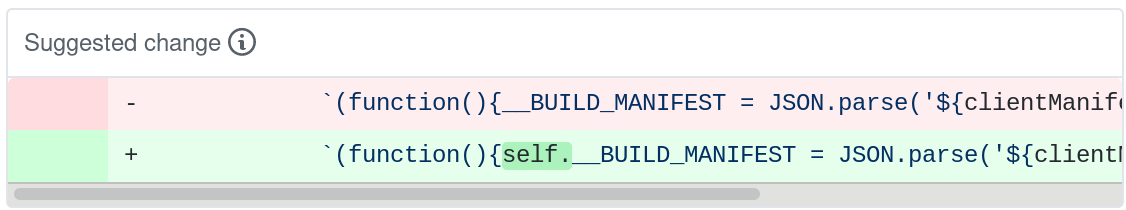
\includegraphics[width=0.75\textwidth]{Chapter-5/images/correct.png} \\
    \textbf{(b) Formatting:} \\
    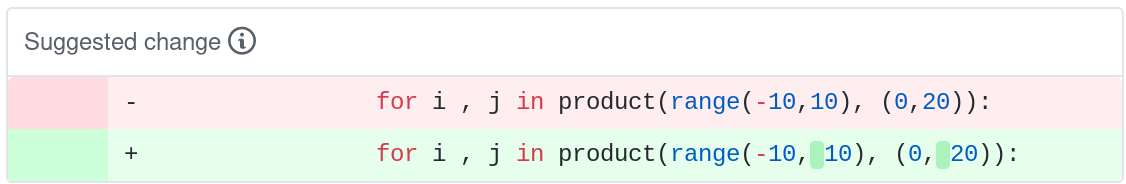
\includegraphics[width=0.75\textwidth]{Chapter-5/images/format.png} \\
    \textbf{(c) Improvement:} \\
    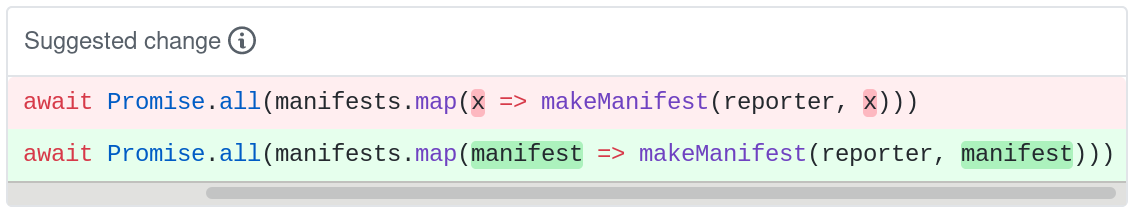
\includegraphics[width=0.75\textwidth]{Chapter-5/images/improve.png} \\
    \textbf{(d) Non-Functional:} \\
    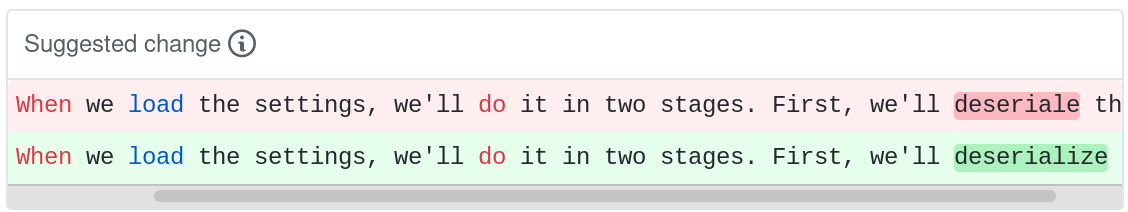
\includegraphics[width=0.75\textwidth]{Chapter-5/images/nonfunc.png}
     
    \caption{Categories of \sugg Results}    
    \label{fig:sugg-categories} 
\end{figure}


\begin{table}[H]
\centering
\caption{\SUGGS Categories Results}
\begin{tabular}{ |c|r|c|} \hline
   & \textbf{\textit{n}} & \textbf{Percentage} \\ \hline
 Non-Functional &  36 & 36\% \\ \hline
 Improvement & 34  & 34\% \\ \hline 
 Corrective &  16 & 16\% \\ \hline
 Formatting & 14 & 14\% \\ \hline
\end{tabular}
\label{tab:sugg-categories}
\end{table}

\subsubsection{RQ2: Effectiveness}

To evaluate the RQ2, we investigated the effectiveness of code recommendation systems on pull requests, specifically \suggs and pull request review comments with fenced code, on the acceptance and timing of pull requests and recommendations. We found that \sugg and review comments with code snippets made up approximately 12\% and 5\% of all pull request review comments in our dataset, respectively. The Pearson’s chi-squared ($\chi^2$) test was used to analyze acceptance while the Mann-Whitney-Wilcoxon test was used to evaluate time.

\paragraph*{Acceptance}

\subparagraph{Contribution Acceptance.}

Overall, 69\% of pull requests in our dataset were merged into repositories ($n$ = 35,521). Table~\ref{tab:sugg-cont-accept} presents the merge rate for pull requests with and without code suggestions from either system. Our results show both groups have approximately the same merge rate, and we found no significant difference in the outcome of contributions based on the existence code recommendations with \sugg or review comments ($\chi^2$ = 0.0182, $p$ = 0.8928, $\alpha$ = .05). Thus, while suggestions are useful for helping developers resolve problems in code reviews, they do not have a major influence on whether pull requests are accepted and merged into repositories.


 \subparagraph{Recommendation Acceptance.} We were also interested in the acceptance rate of recommendations from each system. Overall we found \suggs were much more effective (Table~\ref{tab:sugg-rec-accept}). 60\% ($n = 10,556$) of \sugg were incorporated into pull requests by developers compared to only 1\% ($n =  65$) of review comments with markdown code. Additionally, we found this difference was statistically significant ($\chi^2$ = 6961.3765, p < 0.00001, $\alpha$ = .05). This indicates the \sugg feature is more effective for encouraging developers to adopt recommendations from peers moreso than markdown code presented in pull request review comments.
 
 \subparagraph{} While general code suggestions do not impact the acceptance of contributions on GitHub, we conclude \sugg are effective for proposing improvements to contributors on their pull requests compared to other systems, such as review comments with code.
 %While suggested changes are a relatively new feature, many projects have already adopted the pull-based model for software development on GitHub~\cite{gousios2014exploratory,  gousios2015work}. 


\paragraph*{Timing} 

\subparagraph{Contribution Time.} 

To further evaluate the impact of code suggestions, we measured the amount of time to accept code contributions with \sugg or review comments with fenced code compared to those with neither system. The results, presented in Table~\ref{tab:sugg-cont-time}, show that on average pull requests with code suggestions take over twice as long to merge into repositories. Additionally, we found that pull requests without code suggestions from these systems are merged into repositories significantly faster than contributions with recommendations (W = 87857043, $p$ < 0.00001, $\alpha$ = .05). We deduce contributions with recommendations to developers via \sugg or review comments with code may take longer to be accepted due to increased comments from reviewers, discussions about changes, and time needed to make modifications compared to non-suggestion pull requests.

\subparagraph{Recommendation Time.}

To compare \suggs and review comments with fenced code as mechanisms for recommendations, we analyzed the amount of time for reviewers to comment with suggestions using each system. Our results, displayed in Table~\ref{tab:sugg-rec-time}, show \sugg recommendations are made about four days faster than review comments. Furthermore, this difference in recommendation time is statistically significant between the code suggestion systems (W = 49186174, $p$ < 0.00001, $\alpha$ = .05). This indicates reviewers are able to make recommendations much faster using the \sugg feature compared to code within review comments, allowing developers to provide feedback more efficiently and accelerate the review process.

\subparagraph{Recommendation Acceptance Time.}

Additionally, we analyzed the amount of time for developers to accept recommendations from reviewers using each system. Table~\ref{tab:sugg-rec-accept-time} presents the average acceptance time for developers for \suggs and review comments with fenced code, and we found \sugg are accepted on average three days faster. Our results also show a significant difference in the amount of time taken by developers to incorporate recommendations from each system into their pull requests (W = 256013, \textit{p} = 0.0001, $\alpha$ = .05). This shows \suggs allow developers to evaluate suggestions and make decisions on recommendations quicker than with markdown code in pull request review comments, for example including the ``Commit suggestion'' button to automatically apply changes. 

\subparagraph{} Overall, our timing results show that, while contributions take longer overall to get merged when code is recommended, \sugg facilitate development processes by decreasing the amount of time needed to make suggestions and approve recommendations during code reviews.

 \begin{table}[H]
\centering
\caption{Contribution Acceptance Results}
\begin{tabular}{ |c|r|c| } \hline
  \textbf{Pull Requests} & \textbf{\textit{n}} & \textbf{Rate} \\ \hline
 with suggestions & 6982 & 69.4\%\\ \hline 
 without suggestions & 44268 & 69.3\%\\ \hline
\end{tabular}
\label{tab:sugg-cont-accept}
\end{table}

\begin{table}[H]
\centering
\caption{Recommendation Acceptance Results}
\begin{tabular}{ |c|r|c|} \hline
   \textbf{Type} & \textbf{\textit{n}} & \textbf{Rate} \\ \hline
  suggested changes & 17712 & 59.6\% \\ \hline 
 review comments with code & 6937 & 0.9\% \\ \hline
\end{tabular}
\label{tab:sugg-rec-accept}
\end{table}

\begin{table}[H]
\centering
\caption{Contribution Time (in days) Results}
\begin{tabular}{ |c|r|c|c|} \hline
   \textbf{Type} & \textbf{\textit{n}} & \textbf{Average} & \textbf{Median} \\ \hline
  with suggestions & 6982 & 16.4 & 5.0  \\ \hline 
  without suggestions & 44268 & 6.4 & 1.1 \\ \hline
\end{tabular}
\label{tab:sugg-cont-time}
\end{table}

\begin{table}[H]
\centering
\caption{Recommendation Time (in days) Results}
\begin{tabular}{ |c|r|c|c|} \hline
   \textbf{Type} & \textbf{\textit{n}} & \textbf{Average} & \textbf{Median} \\ \hline
  suggested changes & 17712 & 10.5 & 0.7 \\ \hline 
  review comments with code & 6937 & 14.6 & 1.9 \\ \hline
\end{tabular}
\label{tab:sugg-rec-time}
\end{table}

\begin{table}[H]
\centering
\caption{Recommendation Acceptance Time (in days) Results}
\begin{tabular}{ |c|r|c|c|} \hline
   \textbf{Type} & \textbf{\textit{n}} & \textbf{Average} & \textbf{Median} \\ \hline
  suggested changes & 17712 & 5.4 &  0.3 \\ \hline 
 review comments with code & 6937 & 8.0 & 0.7 \\ \hline
\end{tabular}
\label{tab:sugg-rec-accept-time}
\end{table}


\subsubsection{RQ3: Impact}


To evaluate RQ3, we analyzed the impact of the \sugg feature on pull-based software development by examining its effect on GitHub pull requests. Overall, we analyzed the timing, coding activity, and collaboration between developers. The Mann-Whitney-Wilcoxon test ($\alpha$ = .05) was used to compare characteristics on 4,319 pull requests containing \suggs and 46,931 without recommendations between developers through this system.

\paragraph*{Pull Request Characteristics}

To understand the impact of \sugg on development practices, we analyzed metrics used in prior work to examine pull requests on GitHub~\cite{gousios2014dataset}. These results are presented in Table~\ref{tab:sugg-impact}. Here, we explain specific results based on the pull request characteristics we observed.

\subparagraph{Timing.} Similar to our analysis evaluating the impact of code suggestions on contribution time, we found that pull requests with \suggs take almost twice as long and significantly longer to be accepted (\textbf{\em mergetime\_minutes}, $p < 0.00001$) and closed, with or without merging (\textbf{\em lifetime\_minutes}, $p < 0.00001$). This may be due to the fact that pull requests with \sugg extend reviews and add more time to the code inspection process, have more complex development activity, and more conversations between developers on contributions. 

\subparagraph{Coding Activity.} One reason pull requests utilizing \sugg take longer is because developers are significantly more active on these contributions. We found pull requests with this feature have more commits (\textbf{\em num\_commits}, $p < 0.00001$) and modified lines of code (\textbf{\em src\_churn}, $p < 0.00001$) from contributing developers. However, we found on that average pull requests with this feature impact fewer files. For RQ2, we found \sugg are well-accepted by developers. With this system, developers can automatically apply recommendations from reviewers as additional commits to their pull requests on a line of code within a file, leading to increased commits and code changes to improve the quality of the program.

\subparagraph{Collaboration.} Additionally, our results show that \suggs impact feedback and discussions during code review processes. We found that pull requests with developers using the \sugg feature have significantly more review comments on lines within the submitted code (\textbf{\textit{num\_commit\_comments}}, $p < 0.00001$), general discussion between programmers about contributions (\textbf{\em num\_issue\_comments}, $p < 0.00001$), and developers engaging in conversations about pull requests (\textbf{\em num\_participants}, $p < 0.00001$). This indicates \sugg are a valuable system for providing feedback, facilitating communication between developers, and discussing improvements to pull requests.


\begin{table*}[tbh]
\centering
\caption{Pull Request Impact Results}
\begin{threeparttable}
\begin{tabular}{ |l|l|r|r|c| } \hline
  \textbf{Characteristic} & \textbf{Dataset} & \textbf{Mean} & \textbf{Median} & \textbf{\textit{p-value}} \\ \hline
 \multirow{2}{*}{\textbf{\em lifetime\_minutes***}} & with suggested changes & 34799.26 & 8190.43 & - \\
 & without suggested changes & 18993.48 & 2489.12 & \textbf{$p$ < 0.00001} \\ \hline
 \multirow{2}{*}{\textbf{\em mergetime\_minutes***}} 
 & with suggested changes & 23645.15 & 5900.27 & - \\
 & without suggested changes & 10378.82 & 1776.32 & \textbf{$p$ < 0.00001} \\ \hline
 \multirow{2}{*}{\textbf{\em num\_commits***}} 
 & with suggested changes & 8.62 & 4 & - \\
 & without suggested changes & 6.72 & 1 & \textbf{$p$ < 0.00001} \\ \hline
 \multirow{2}{*}{\textbf{\em src\_churn***}} & with suggested changes & 866.86 & 133 & - \\
 & without suggested changes & 3212.64 & 26 & \textbf{$p$ < 0.00001} \\ \hline
 % \multirow{2}{*}{test\_churn}  & with suggested changes & & & - \\
 % & without suggested changes & & & \\ \hline
 % \multirow{2}{*}{files\_added} & with suggested changes & & - \\
 % & without suggested changes & & & \\ \hline
 % \multirow{2}{*}{files\_deleted}  & with suggested changes & & & - \\
 % & without suggested changes & & & \\ \hline
 % \multirow{2}{*}{files\_modified}
 % & with suggested changes & & & - \\
 % & without suggested changes & & & \\ \hline
 \multirow{2}{*}{files\_changed}
 & with suggested changes & 7.71 & 2 & - \\
 & without suggested changes & 11.54 & 2 & $p$ = 0.5051 \\  \hline
%  \multirow{2}{*}{src\_files} 
%  & with suggested changes & & & - \\
%  & without suggested changes & & & \\ \hline
 %\multirow{2}{*}{doc\_files} & with suggested changes & & & - \\
 %& without suggested changes & & & \\ 
 %& \textit{pullReqs} & 2.36 & 0.00 & \\\hline
 %\multirow{3}{*}{other\_files} & with suggested changes & & & \\
 %& without suggested changes & & & \\ 
 %& \textit{pullReqs} & 2.74 & 0.00 & - \\ \hline
 \multirow{2}{*}{\textbf{\em num\_commit\_comments***}} & with suggested changes & 13.56 & 7 & - \\
 & without suggested changes & 2.00 & 0 & \textbf{$p$ < 0.00001} \\\hline
 \multirow{2}{*}{\textbf{\em num\_issue\_comments***}} & with suggested changes & 8.63 & 5 & - \\
 & without suggested changes & 5.03 & 3 & \textbf{$p$ < 0.00001} \\ \hline
 \multirow{2}{*}{\textbf{\em num\_participants***}} & with suggested changes & 3.18 & 3 & - \\
 & without suggested changes & 2.30 & 2 & \textbf{$p$ < 0.00001} \\ \hline

\end{tabular}
\begin{tablenotes}
\centering
\textbf{***} denotes statistically significant results (\textbf{p-value < 0.05})
\end{tablenotes} 
\end{threeparttable}
\label{tab:sugg-impact}
\end{table*}

\subsubsection{RQ4: Usefulness}

To study RQ4, we surveyed developers to collect feedback on the \suggs feature. Of the 43 survey responses we received, 24 responses from were from developers who received suggestions and 19 responses were from users who made a recommendation. Here we present the results from analyzing 5-point Likert scale responses and open-ended replies from developers.

\subparagraph{Likert Scale.} 

Figure~\ref{fig:sugg-usefulness} displays the results of the Likert scale asking developers how useful they found the \sugg feature. Overall, we found 92\% of suggestees ($n = 22$) and 79\% of suggesters ($n = 15$) reported \suggs are Useful or Very Useful. Furthermore, no developer who interacted with this system reported that it was Not at All Useful. One participant (\ser12) ranked the system as Somewhat Useful due to the fact that \sugg incorporate accepted suggestions as individual pull request commits and desired a ``force push'' option to squash all of the commits and better adhere to their team's development workflow. Overall, our results show GitHub users find this feature effective for both receiving recommendations as well as making suggestions to developers on GitHub. 

% \vspace{-0.75em}

\subparagraph{Qualitative Feedback.}

To further examine \suggs, we asked surveyed developers to provide open-ended responses describing what they find useful or unuseful about suggested changes. Two researchers conducted an open coding on free response feedback to derive themes describing how developers perceive this feature. The main negative feedback received about \sugg focused on the limitations of the system (i.e. ``\textit{no multiline support}'' (\ser1)), its conflicts with other development tools (i.e. ``\textit{approval process handlers like PullApprove and Zappr now will not recognize my approval of the PR}'' (\ser16)), and the functionality of applying suggestions as separate commits (i.e. ``\textit{Some changes could be grouped in a single commit...[individual commits] is less convenient}'' (\see9)).\footnote{At the time of this experiment, \suggs only supported single line changes. However, after the study date GitHub has since updated the feature and introduced \sugg for multiple lines (\url{https://github.blog/changelog/2020-02-26-multi-line-code-suggestions-beta/}).} We extracted eight themes from our analysis to describe what developers found useful about \suggs. Below, we define each category derived from the qualitative coding and provide example responses to summarize developer feedback on the advantages and disadvantages of \sugg: \\

\textbf{\textit{Actionability:}} Developers reported finding \sugg useful because of the actionability of recommendations from this system. This refers to ability for users to automatically act on recommendations from reviewers and commit proposed code changes into their on pull requests. Survey respondents frequently lauded the fact that \sugg are are actionable and easy to integrate into code review processes.

\begin{quote}
    \textit{``the fact that small changes can be applied immediately, and the fact that they can be described by the reviewer in a way that a button fixes it instead of going to your code''} (\see3)
\end{quote}

\textbf{\textit{Communication:}} Participants also reported that \suggs are effective for communication between developers. This refers to the capability of developers to understand recommendations and the transfer knowledge between peers through this system. Our survey feedback suggests \sugg provide a mechanism for clear communication between developers and reviewers during the code review process.

\begin{quote}
    \textit{``We can understand reviewer's intention more. If not using this feature, there are only pull request comment text, so we may misunderstand reviewer's intention''} (\see16)
\end{quote}

\textbf{\textit{Code:}} Users also found the \suggs feature useful is because it allows reviewers to make recommendations as code. Several participants mentioned they preferred the ability to give and receive suggestions using code rather than writing out recommendations as text in pull request review comments.

\begin{quote}
     \textit{``It is very convenient that the reviewer can write what they suggest to change in code instead of formulating it in words (which will often be longer)''} (\ser6)
\end{quote}

\textbf{\textit{Conciseness:}} Similarly, participants also appreciated the brevity of recommendations with \sugg. Many developers found the concise code recommendations to be useful for easily making and reacting to suggestions when using this system. Examples of this can found in responses such as the one below where a suggester found suggested changes useful because they can:

\begin{quote}
    \textit{``Suggest small one line changes directly and concisely''} (\ser9)
\end{quote}

\textbf{\textit{Ease of Use:}} Respondents also noted that recommendations with \sugg are effective because the system is easy for suggesters and suggestees to use. Feedback from participants commended this feature for its intuitive interface design and ability to effortlessly integrate into the pull request review process.

\begin{quote}
    \textit{``It's really easy to use, it's really easy to accept the suggestion so some works are really easy''} (\see15)
\end{quote}

\textbf{\textit{Location:}} Participants also found the location, or where \sugg recommendations are made, useful for making and receiving suggestions. We found developers liked the ability to make recommendations directly on the line of code to be improved. For example, one respondent mentioned this feature is useful because there is:

\begin{quote}
    \textit{``No need to leave the pull request page to make a suggested change, [and it's] easy to see what is being suggested''} (\ser12)
\end{quote}


\textbf{\textit{Scalability:}} Another reported benefit of \sugg is the ability of this feature to make and receive numerous recommendations on the same pull request. Users found the scalability of this system useful, especially for reviewing code and making several recommendations to developers on the same pull request during reviews.

\begin{quote}
    \textit{``It...gives me the ability to suggest multiple options during review''} (\ser11)
\end{quote}

\textbf{\textit{Timing:}} Developers also found the timing of \sugg makes them useful. For example, many participants mentioned this feature improves the speed with which users can make and address recommendations on pull requests and also noted its overall impact on accelerating the code review process.

\begin{quote}
    \textit{``Being allowed to add specific changes speeds up the review process. Sometimes it is easier to make the changes yourself rather than make a suggestion and wait for a change''} (\see17)
\end{quote}

\textbf{\textit{No Response:}} Several participants who completed the survey did not respond to the free response question to provide feedback on the usefulness of \suggs. This question was optional in the survey, and we cannot conclude the reason developers chose not to respond is due to not finding anything useful about the feature.

\begin{figure}[htb]
\centering
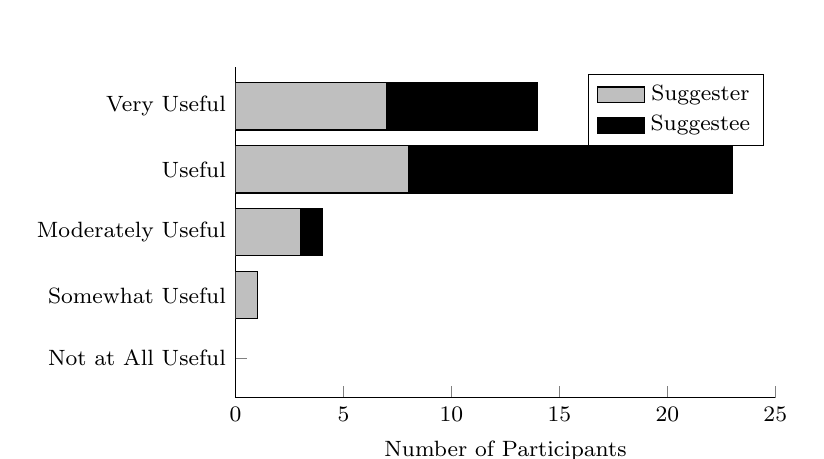
\begin{tikzpicture}
\begin{axis}[
    xbar stacked,
    ytick=data,
    axis y line*=none,
    axis x line*=bottom,
    tick label style={font=\footnotesize},
    legend style={font=\footnotesize},
    label style={font=\footnotesize},
    xtick={0,5,10,15,20,25},
    %width=.4\textwidth,
    bar width=6mm,
    xlabel= Number of Participants,
    yticklabels={Not at All Useful, Somewhat Useful, Moderately Useful, Useful, Very Useful},
    xmin=0,
    xmax=25,
    area legend,
    y=8mm,
    enlarge y limits={abs=0.625},
]
% Suggesters
\addplot[fill=lightgray] coordinates
{(0,0) (1,1) (3,2) (8,3) (7,4)};
% Suggestees
\addplot[fill=black] coordinates
{(0,0) (0,1) (1,2) (15,3) (7,4)};
\legend{Suggester, Suggestee}
\end{axis}  
\end{tikzpicture}
\caption{Survey Results on the Usefulness of \suggs}
\label{fig:sugg-usefulness}
\end{figure}


\subsection{Summary}

Our findings show that \suggs have a major influence on development practices and behavior. We discovered this feature is useful for suggesting different types of code changes, effective for facilitating recommendations during reviews, and beneficial for improving coding activity and collaboration between developers. Additionally, we found developers find \sugg useful for making and receiving recommendations on GitHub pull requests. Based on qualitative analysis examining user feedback on the advantages of \sugg, we submit two main implications for improving the future recommender systems and their developer impact. These implications include incorporating \textbf{\em user-driven communication} (\textit{Communication}, \textit{Code}, and \textit{Conciseness}) and \textbf{\em workflow integration} (\textit{Actionability}, \textit{Ease of Use}, \textit{Location}, \textit{Scalability}, and \textit{Timing}) into automated recommendations to improve developer behavior.

\section{Discussion}

To evaluate \framework, this work analyzes \suggs as a recommendation system incorporating all the principles from this conceptual framework. The findings from the evaluations of \sugg presented in this chapter show that developers prefer to receive recommendations from this system and it has a major impact on development practices on GitHub. Overall, we provide four implications for designing effective recommender systems based on the results of these studies: \textbf{\em recommendation content}, \textbf{\em recommendation design}, \textbf{\em user-driven communication}, and \textbf{\em workflow integration}. Here, we explain these conclusions from the context of each study and through the lens of the \framework framework.

\subsection{Actionability}

Our analysis of the \suggs feature suggests that actionability influences the perception and adoption of recommendations by developers. For example, the recommendation styles and developer impact study offer \textit{recommendation design} and \textit{workflow integration} as implications to improve automated suggestions from future recommender bots. To describe the impact of actionability in \sugg, I describe themes derived from qualitative feedback from developers in the studies presented in this chapter.

\subsubsection*{Workflow Details}

The recommendation styles results show that \textit{integration} details within the content of automated suggestions can influence adoption. These workflow details, describing how to install and integrate tools into development processes, also contribute to the actionability of recommendations by providing information on how easy it is to adopt tools and practices. For example, participants mentioned they were interested in learning if suggested tools would easily work with ``\textit{whatever CI or test runner system I've got}'' (P8) and wanted to know if they had ``\textit{simple integration}'' (P1). Similarly, developers desired information on the \textit{reliability} of systems to learn about their stability and how well tools do the things they claim to do.

Furthermore, participants mentioned designing automated recommendations to include relevant \textit{examples} of usage. For instance, P14 stated ``\textit{specific examples...would be a lot more compelling}'' and P10 noted ``\textit{It would be better if they can show me some examples with some very clear results like this is something you can get with our tool}''. Additionally, developers were interested in testing out the actionability of recommendations saying  ``\textit{I would like to try it by myself first}'' (P11) and ``\textit{I would test it out locally}'' (P8). By incorporating details on the actionability of recommendations this concept into developer recommendations such as how to install tools, integrate them into CI build systems, and the existence of plugins within popular IDEs, automated recommendations can increase the likelihood of adoption for developer behaviors. 


\subsubsection{Workflow Integration} 

Both \suggs studies show the importance of integrating recommendations effectively into developer workflows. For instance, developers were likely to adopt tool recommendations from \sugg over other recommender systems because of its ability to automatically apply recommendations and its ``neat integration'' (P7). Our preliminary work also shows that integration is a key factor in developer adoption, with the disruptiveness of notifications from \toolone discouraging users from adopting recommendations. However, we found developers were more likely to adopt automated static analysis tool recommendations from actionable systems such as \suggs. 

The developer impact study also found actionability increased adoption of code change suggestions. We found \sugg were more popular and more effective than static pull request review comments with fenced code. Our qualitative results also showed this was one of the most useful aspects of this recommendation system. For example, participants mentioned they found ``\textit{the ability for people to be able to suggest changes and to be able to incorporate those changes immediately}'' (\see8) and the fact suggestions can be ``\textit{accepted right away, without requiring copy pasting and committing on my side}'' (\see9) useful for receiving recommendations. Additionally, developers reported \textit{ease of use} and \textit{scalability} contributed to the ability to easily adopt \sugg into code review processes and make suggestions to developers. Hence, we show actionability can enhance automated recommendations and improve the effectiveness of recommender systems.

\subsection{Feedback}

The \sugg studies also show that the information provided to users in automated recommendations impacts adoption. For example, we found \textit{recommendation content} influences the style of automated recommendations and \textit{user-driven communication} is a favorable aspect of \suggs. To illustrate the importance of feedback in recommendations with this system, I outline themes provided by developers from the results of the recommendation styles and developer impact studies. 

\subsubsection{Relevance}

Developers in the recommendation styles study reported details concerning the relevance of tools impacts their decisions on adoption. For instance, P2 mentioned the content of recommendations helps them decide whether ``\textit{it's something I really need or want}'', P9 stated ``\textit{the recommendation itself matters less than how much I need the thing...If I don’t need it then I’m not going to try it}'', and P12 declared they ``\textit{don't really care}'' about tools that are irrelevant to their work. Participants were specifically interested in receiving information about integration details, the reputation of tools, and the trustworthiness of systems. Alternatively, irrelevant recommendations that ``\textit{show some other useless stuff which may confuse the potential user}'' (P10) can lead to ineffective recommendations. For example, we found \tele suggestions were not useful because they provided irrelevant and generic feedback in recommendations to users.

Similarly, developers expressed disdain for recommendation content that appears to be \textit{marketing} or advertisements. For example, developers described the email recommendation stating it sounds ``\textit{pretty suspicious}'', ``\textit{email...there’s so much stuff that comes through email}'' (P1), ``\textit{email is definitely a no}'' (P7), and ``\textit{I'd immediately delete it}'' (P6). Additionally, P5 mentioned ``\textit{I’m not somebody who likes to get unsolicited marketing stuff}''. The negative perception of marketing in software engineering can also be found from the backlash received by maintainers of the StandardJS JavaScript style guide, linter, and formatting tool,\footnote{\url{https://standardjs.com/}} who attempted to raise funds for development by incorporating advertisements inside the terminal.\footnote{\url{https://github.com/standard/standard/issues/1381}} In this instance, we found poor feedback in suggestions discouraged users from adopting recommendations and contend automated systems should avoid marketing language in recommendations.

However, we found details about the \textit{popularity} of systems plays a key role in adoption according to participants in the recommendation styles study. Most developers desired information the reputation of tools when making decisions, stating ``\textit{one of the things I want to see is what other people think about it}'' (P3), ``\textit{how many people use it...the popularity of the tool being used would influence me to try that}'' (P6), ``\textit{when there’s a buzz around a tool, that’s when you know it’s good and you know it’s worth checking out}'' (P12), and recommendations should ``\textit{try to highlight the popularity, popularity is so crucial}'' (P13). 

Participants also mentioned using various sources for learning about the reputation of tools, such as from peers (i.e. ``\textit{word of mouth and people that I actually trust who use it}'' (P6)) and online searches (i.e. ``\textit{Google the tool's name...[and get] a link on the first page}'' (P5)) in addition to social media and other online programming communities. Prior work also shows displaying details about popularity impact adoption of developer behaviors, such as increasing updates to repositories and contributions from collaborators~\cite{aggarwal2014co}. This indicates automated recommendations should consider incorporating popularity statistics such as number of users, downloads, social media followers, and reviews to encourage adoption. Thus, we argue including relevant feedback about tools and practices is necessary to encourage the adoption of developer behaviors

\subsubsection{Conciseness}

The recommendation styles and developer impact study found users appreciated the brief and compact nature of recommendations with \suggs. For example, when describing the email and issue static analysis tool recommendations mentioned they contained ``\textit{a ton of words}'' and were ``\textit{way too lengthy}'' (P13). Additionally, P10 noted effective recommendations ``\textit{just get[sic] to the point}''. However, P8 liked \sugg because they provide a ``\textit{nice, concrete error}'' (P8). Even though all of the recommendation styles contained similar text in the suggestion, systems such as email appeared to contain more text for developers to read. Likewise, research suggests software engineers prefer instant messaging systems because they are more concise and quicker than emails~\cite{blatt2013email}.

\textit{Concise} recommendations with \suggs also played a role in impacting developer behavior. For example, \ser11 noted ``\textit{it uses less words}''. Developers also reporting preferring recommendations as \textit{code} stating this system ``\textit{can quickly and precisely show what change they expect. Describing the change with words is pretty annoying}'' (\see12), ``\textit{removes guesswork from interpreting a prose explanation}'' (\ser4), and ``\textit{removes all ambiguity about what I'm asking for if I can just directly put the code there}'' (\ser12). Prior work also found conciseness is important designing interactive software systems~\cite{wasserman1981user} and in \textit{quick fix designs} to increase adoption of code-checking systems~\cite{Johnson2013Why}.

\subsubsection{Communication}

The developer impact study results show one of the most useful aspects of \sugg is their ability to effectively communicate to developers. Participants found this system effective for facilitating clear communication between developers on pull requests. For instance, users replied this system is useful because it ``\textit{lets someone else directly make changes instead of writing out instructions on how to make changes}'' (\see10), ``\textit{gives the suggestion in a very clear way}'' (\ser5), and provides ``\textit{easy information on what to change in your pull request}'' (\see5). This \textit{user-driven communication} led to effective recommendations from developers on pull requests. Prior work also suggests poor communication from automated systems prevents static analysis tool adoption~\cite{Johnson2013Why} and frustrates developers during interactions with bots~\cite{wessel2018power}, while \textit{user-driven conversations} improves the effectiveness of recommender chatbots~\cite{cerezo2019building} while specific and clear language can overcome barriers to security adoption adoption~\cite{Xiao2014Security}. We propose implementing clear communication focused on users to improve automated developer behavior recommendations. Overall, we conclude developers are more likely to adopt recommendations with relevant, concise, and clear feedback.


\subsection{Locality}

\suggs provide support recommendation locality because of their ability to situate suggestions on lines of code and present recommendations during code reviews. We found this \textit{recommendation design} for the placement and timing of notifications increased the likelihood of developers adopting behaviors. These related findings from our studies are presented below.

\subsubsection{Timing} For the recommendation styles user study, we found the systems with more convenient temporal locality (\suggs) were more likely to convince developers to adopt static analysis tools than those with low temporal locality (pull requests, issues, and emails). We refer to these systems as having low temporal locality because, unlike \sugg, they can appear to developers in their email or repository any time during the development process. However, \sugg are limited to open pull requests currently under review. Similarly, previous research in software engineering shows untimely recommendations prevented programmers from adopting code navigation recommendations from Spyglass~\cite{viriyakattiyaporn2009challenges} while timely notifications increased the amount of Infer\footnote{\url{https://fbinfer.com/}} and Zoncolan\footnote{\url{https://engineering.fb.com/2019/08/15/security/zoncolan/}} static analysis warnings by developers at Facebook~\cite{Distefano2019Facebook}.

In the developer impact study, many survey respondents commented on how \suggs impacted the timing of reviews. For example, developers mentioned this feature ``\textit{lets me do reviews much faster}'' (\ser3), ``\textit{accelerates getting pull requests accepted}'' (\see4), ``\textit{it's great to be able to quickly apply changes}'' (\see23), and ``\textit{it's often quicker both to suggest a minor change}'' (\ser8). Our quantitative analysis also found that, while \sugg lengthen the overall pull request review process, they are significantly faster for making recommendations and responding to suggestions during the code review process. Therefore, to design effective automated recommendations, systems should focus on making suggestions to developers at convenient times within the development workflow. 

\subsubsection{Location}

Our recommendation style study results also suggest that the placement of notifications is important for developer recommendations. For example, we found participants were least likely to adopt recommendations from emails, the system with the worst spatial locality in a separate window outside of the repository. As the spatial locality of recommendations improved, we found developers were more likely to adopt static analysis tool recommendations with \suggs, the most conveniently located notification on the line of code, being the most effective. P5 also mentioned the location of recommendations influences their decision on whether or not to adopt, noting they did not want to ``\textit{go to [the tool's] website and have to click through a million different links}''. Prior work shows tool recommendations within the coding panels of IDEs can increase efficiency and are preferred by developers~\cite{Flower} in addition to minimizing \textit{visual momentum} and helping programmers feel less disoriented in their development environment~\cite{de2006using}.

Participants in the developer impact study also praised the location of \sugg. For example, \see24 stated this feature is useful because there is ``\textit{no need to leave the pull request page to make a suggested change}''. GitHub developers also added this feature is useful because it ``\textit{shows suggested code changes integrated with the actual source}'' (\see22) and ``I can just directly put the code there'' (\ser 13). Thus, we argue automated recommendations should appear at convenient locations within the programming environment in order to increase the likelihood of adoption and improve the behavior of developers. \\

Overall, the results of the \suggs studies show that this system is preferred by developers for receiving recommendations and effective for improving development practices. This system, which incorporates the \framework framework, uses this framework to make actionable, relevant, clear, and convenient recommendations to developers. The feedback provided from developers through semi-structured interviews and surveys confirm the presence of these framework principles contribute to the effectiveness of \sugg on GitHub. Ultimately, we conclude \framework is a useful mechanism for creating automated recommendations because of its focus on recommendation content and design as well as fostering user-driven communication and facilitating workflow integration.









\chapter{ Designing New Recommender Bots }
\label{chap-bot}

Based on findings from the previous chapter, automated recommendations containing \framework are preferred by software engineers and influence their development practices. The studies presented analyzed \framework through the \suggs feature, and show that developers are more likely to adopt tool recommendations from systems incorporating this framework~\cite{RecommendationStyles} in addition to showing the suggestions made through this feature are effective for making and receiving code improvement recommendations and improving the coding activity and collaboration of peers on pull requests~\cite{SuggUnderstanding}. However, the thesis of this dissertation argues that \framework is able to improve code quality and developer productivity. To investigate this claim, I developed a new system, \tooltwo, that incorporates each of the design principles from this conceptual framework and present an evaluation of this system exploring its impact on the quality and productivity of programmers' work. Study materials for this work are available in Appendix~\ref{app-bot}.

\section{Study Rationale}

Undergraduate Computer Science courses are constantly evolving to handle the significant increase of students~\cite{Kay98Intro}. For example, educators have turned to many different automated tools to complete instructional tasks such as grading assignments and generating feedback on student code~\cite{Wilcox2015Automation}. However, studies show that despite increasing enrollment and the advantages of automated systems in the classroom, the dropout out rate in Computer Science, especially among first and second year students, is also growing. Beaubouef and colleagues suggest a primary reason for high attrition in these courses is poor behavior, such as ignoring software development processes, on programming assignments~\cite{beaubouef2005high}. To further explore the impact of \framework on improving developer behavior, this work seeks to apply this framework to make recommendations to students on programming projects. Decision-making is vital in software engineering~\cite{WooDecision}, however students frequently make poor choices and adopt bad programming behaviors when writing code for projects~\cite{Edwards09Behaviors}. Furthermore, these behaviors persist among professional software engineers who also often underestimate the time and effort required to complete development tasks~\cite{Boehm1984SEEcon}, leading to further problems such as inadequately tested software~\cite{Whittaker00Testing} and insufficient documentation~\cite{Briand03Documentation}.

\subsection{Research Questions}

To examine the impact of digital nudges for improving the behavior of students on programming assignments, we seek to answer the following research questions:

\begin{itemize}[topsep=0pt,itemsep=-1ex,partopsep=1ex,parsep=1ex]
  \item[\textbf{RQ1}] How do nudges impact the quality of student projects?
  \item[\textbf{RQ2}] How do nudges influence student productivity?
\end{itemize}

To answer these questions, I performed a study implementing \tooltwo, a system that utilizes \framework to recommend beneficial software engineering behaviors to students, on projects for an introductory undergraduate programming course. The effectiveness of this system was evaluated by examining the code quality of projects and the productivity of students. Our results suggest automated nudges from \framework improved performance, increased coding activity, and prevented procrastination on assignments. The contributions of this research include \tooltwo, a novel bot for recommend software engineering practices to students on coding projects, and an evaluation of \framework this system on improving the software engineering behaviors of student programmers.

\section{\tooltwo: Implementing \FrameWork}

To analyze automated approaches for improving programmer behavior, this work posits \tooltwo. The \tooltwo system nudges students to improve their behavior on programming assignments by automatically generating and updating issues on project GitHub repositories. This bot, presented in Figure~\ref{fig:class-bot}, utilizes GitHub issues because they allow developers to manage bugs, suggest enhancements, and provide feedback on repositories~\cite{Issues}. Furthermore, prior work suggests the GitHub issue tracker is useful for making recommendations to developers~\cite{bissyande2013issues}. 

To improve student programming behaviors, \tooltwo encouraged them to follow the \textit{software development process}, or set of activities necessary to develop and maintain software applications. This procedure includes activities related to the \textit{Requirements}, \textit{Design}, \textit{Implementation}, \textit{Testing}, and \textit{Deployment} of software. Prior work suggests students failing to follow the software development process leads to high attrition in undergraduate Computer Science courses~\cite{beaubouef2005high}. The generated issues from \tooltwo on student repositories contained sections for each software development process phase. For example, the 
\includegraphics[height=1em]{Chapter-6/images/rq.png} icon in Figure~\ref{fig:class-bot} represents the Requirements phase and activities related to understanding project guidelines, such as adding a description in the README. In each section, this system outlined rubric items for the assignment relevant to each phase. 

Automated issues from \tooltwo fit the definition of a nudge because they do not provide incentives to students for completing tasks nor prevent students from avoiding items. This system was evaluated against a baseline approach of using an online rubric to illustrate project requirements and the software phases.\footnote{An example of the online rubric is available here: \url{https://pages.github.ncsu.edu/engr-csc116-staff/2020-summer/projects/project6/rubric}} To improve the programming behaviors of undergraduate Computer Science students, \tooltwo was designed using \framework: \textit{Actionability}, \textit{Feedback}, and \textit{Locality}~\cite{Sorry2}. Below, we explain how \tooltwo incorporates each principle to improve student adherence to software engineering process phases.

\subsection*{Actionability}

Actionability involves automating tasks to encourage the adoption of developer behaviors and reducing user effort. \tooltwo incorporated this principle by programmatically analyzing project repositories to determine if students complete certain development process tasks according to the rubric. If the tool observes an item was accomplished based on recent commits to the project, then \tooltwo automatically updated the issue to indicate the task was completed. For example, the system would automatically run the unit tests for the code to determine if a project's unit tests were passing the system or validate a .gitignore file was pushed to the repository to verify the configuration file was added. Alternatively, the baseline approach was not actionable as the online rubric required students to manually seek information and compare their development progress to the assignment requirements outlined on the website.

\subsection*{Feedback}

Feedback consists of providing clear and coherent information to users in automated notifications. \tooltwo implements a simple feedback mechanism to present information to students on their adherence to software engineering processes. The system displayed a red x (
\includegraphics[height=1em]{Chapter-6/images/x.png}) if the assignment requirements for a project task were not completed. When the bot detected a task was completed, it automatically updated the feedback icon next to the rubric item listed in the GitHub issue to be a green check mark (
\includegraphics[height=1em]{Chapter-6/images/check.png}). For instance, in the Deployment phase of the \tooltwo example in Figure~\ref{fig:class-bot}, the project repository does contain a .gitignore file but the source code does not compile. However, with the baseline approach students were not provided with any feedback on their project and were forced to determine if project expectations are met on their own.


\subsection*{Locality}

Locality refers to the setting of automated recommendations, specifically when and where interventions are displayed to users during the development processes. To promote \textit{spatial locality}, \tooltwo recommendations were implemented as GitHub issues located on the project repository within the issue tracker. To support \textit{temporal locality}, the system automatically analyzed repositories daily to provide regular updates to the \tooltwo software development processes issues based on students' recent commits and code contributions to their project. However, the baseline approach does not incorporate temporal or spatial locality in that it forced students to search for information at a separate location from their repository on the course website and in ad hoc manner without any specified timing.

\begin{figure}[htbp]
\centering
	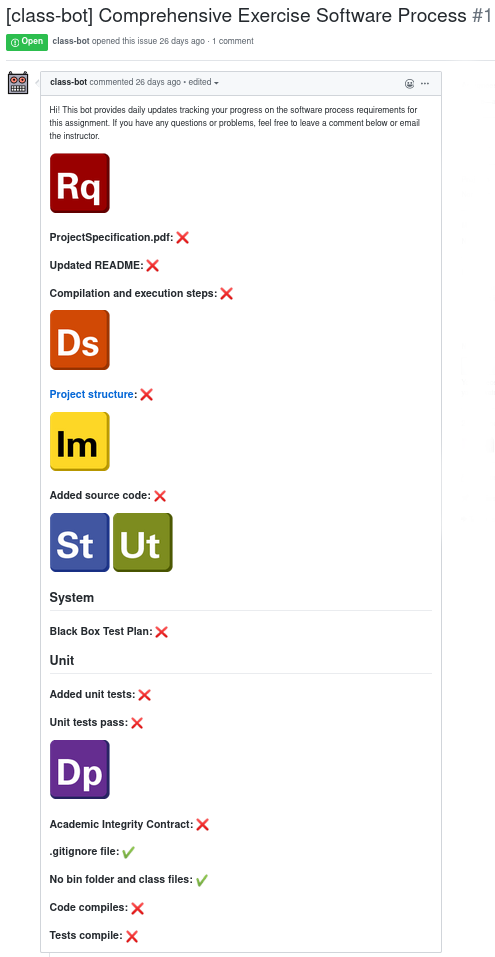
\includegraphics[width=0.65\textwidth]{Chapter-6/images/class-bot1162.png}
	\caption{Example \tooltwo recommendation}	
	\label{fig:class-bot} 
\end{figure}

\section{Methodology}

To explore the impact of digital nudges on code quality and developer productivity, we implemented a mixed methods study to analyze \framework on student behavior for projects in a university-level introductory Java programming course.

\subsection{Data Collection}

\subsubsection{Participants} 

Participants were undergraduate students enrolled in an introductory Java programming class. The students were from different majors, demographics, and levels of programming experience. For consistency in our data, students who enrolled and then eventually dropped the class were eliminated from this evaluation. Overall, we observed the behavior of 35 out of the initial 42 registered students. The participants were aware of the five phases used to define the software development process: \textit{Requirements}, \textit{Design}, \textit{Implementation}, \textit{Test}, and \textit{Deployment}, as presented to students in the course curriculum.

\subsubsection{Projects}

To analyze \framework in \tooltwo, we observed and nudged developer behaviors to students on introductory Java programming projects. For the semester the course consisted of seven programming assignments, six projects and a final comprehensive exercise. Projects 3-5 made up the control group for this experiment to avoid the beginning assignments (Projects 1 and 2). \tooltwo was introduced to students on the final two assignments of the course, Project 6 and the Comprehensive Exercise, to examine its impact on the quality of projects and productivity of students. All coding projects for the were hosted and submitted on GitHub repositories. In total, we analyzed a total of 151 projects from students.

\subsubsection{Developer Behavior}

To improve the decision-making of programmers, the developer behavior \tooltwo focused on encouraged students to follow the software engineering process. Prior work by Beaubouef and colleagues suggests students' failure to adhere to development processes factors into the high attrition rate and failure rate in early programming courses. For example, they note the following about typical student programming methods:

\begin{quote}
``\textit{This [students' estimated time to complete projects] minimally includes the processes of analysis, design, coding, testing, and documentation. Software projects developed by professionals are notoriously behind schedule in the real world. It should come as no surprise that software developed (programs written) by students will tend to be even more behind schedule.} 

\textit{Unsuccessful students often want to skip analysis and design and begin typing in code immediately. Documentation is an afterthought at best, and little or  no testing is performed. Because the student planned to attack the assignment in this manner from the beginning, he will often wait until the last minute to begin and work until its done or time runs out. These students set themselves up for frustration, unnecessary rework, and failure.}''~\citep[p.~105]{beaubouef2005high}
\end{quote}

We define the software development process as \textit{Requirements}, \textit{Design}, \textit{Implementation}, \textit{Test}, and \textit{Deployment}. These phases were derived from the course materials and introduced to students during a lecture before \tooltwo was introduced on projects for this study. Our goal is to use \framework to encourage students to complete all of the software process phases for their projects. Each project contained a \tooltwo issue with sections for each phase listing the relevant tasks. Specific items listed differed based on the project requirements, however in general: Requirements (\texttt{Rq}) focused on activities to understand assignment specifications; Design (\texttt{Ds}) referred to the organization of code and project structure; Implementation (\texttt{Im}) centered on the development of the code; Testing concentrated on actions to develop unit tests (\texttt{Ut}) and functional test cases (\texttt{St}); and Deployment (\texttt{Dp}) concentrated on actions to verify the project and repository were ready for submission. When students completed a specific task, \tooltwo would automatically update the issue to indicate the item was completed.

\subsection{Determining the effectiveness of \tooltwo}

To examine the impact of \tooltwo on student behavior, we mined GitHub repositories to observe metrics measuring its impact on the quality of students' work and the productivity of their project development.

\subsubsection{Quality}

To answer RQ1, we evaluated the quality of student projects by examining their overall \textit{grade} on the assignment in addition to the number of \textit{points deducted} from the project due to students not adhering to requirements for the assignment.

\paragraph*{Grade}

For coding projects, the assignment grade indicates the overall quality of the project. Research suggests poor project management skills~\cite{beaubouef2005high} and ineffective behaviors~\cite{Edwards09Behaviors} result in low grades for students on programming assignments. Similarly, research shows the behavior and \textit{software process maturity} impacts the quality of programs for professional software engineering teams~\cite{Clark97theeffects}. Within the course analyzed for this study, project grades were determined by real-world software engineering quality metrics, such as passing unit tests and functional test cases, Checkstyle\footnote{\url{https://checkstyle.sourceforge.io/}} static analysis tool warnings, and correct project structure. To determine how well \tooltwo supports students in software process decisions, we analyzed projects with and without nudges from this system to determine how this approach impacted the overall grade of coding assignments as a method to determine the project quality.

\paragraph*{Deductions}

Another determinant of project quality is the number of points deducted on student programs. In education, grading penalties are commonly used to encourage students to perform better on assignments~\cite{Reeves2017SpecialTW}. Students who failed to meet certain requirements designated for the project had additional points subtracted from their overall grade. For example, submitting an assignment within 24 hours after the deadline resulted in a -10\% late penalty. In this study, we analyzed projects with and without notifications from \tooltwo to determine if \framework improves student behavior and project quality by minimizing the number of points deducted from programs.

\subsubsection{Productivity}

To answer RQ2, this study examines if nudges impact the productivity of students working on programming assignments.
We measured productivity by observing several different metrics mined from GitHub repositories, including the total \textit{number of commits}, \textit{code churn}, the amount of time until the \textit{first commit}, and the timing
between the \textit{last commit} and the assignment deadline.

\paragraph*{Commits}

GitHub commits are used to record specific changes
made to the project files.\footnote{\url{https://docs.github.com/en/desktop/contributing-and-collaborating-using-github-desktop/committing-and-reviewing-changes-to-your-project\#about-commits}} Prior work in Computer Science education explores analyzing repository commits on version control systems to encourage students to make more frequent contributions to projects~\cite{Singer12Race} and predict student performance~\cite{sprint2019mining}. In industry, commits have been used to measure contributions from programmers as well as the prolificacy of developers on GitHub~\cite{Vasilescu2016Multitask}. To discover if nudging students enhances productivity, we compared the total number of commits submitted by students to their project repositories with and without \tooltwo notifications.

\paragraph*{Code Churn}

To determine the impact of automated nudges from
our system on the activity of students, we also analyzed the code churn of commits made to repositories on assignments with and without updates from \tooltwo. Prior work in software engineering suggests code churn is a useful metric measuring effort and the impact of code changes~\cite{Munson98Churn}, predicting the defect density in software~\cite{nagappan2005DefectDensity}, and analyzing GitHub contributions in the pull-based software development model~\cite{gousios2014dataset}. In this evaluation, code churn was measured by summing the number of lines added, deleted, or modified for each commit made by students to their project repository.

\paragraph*{First Commit} To further investigate the impact of \tooltwo on the productivity of students, we analyzed the timing of commits. We examined the timing of the first commit on repositories to indicate when students began development on their project. Prior work by Edwards et al. shows that students who start working on assignments earlier receive significantly higher grades on projects, while students who start later often perform worse~\cite{Edwards09Behaviors}. To calculate the first commit time, we measured the amount of time between the creation and designation of project repositories to students after the assignment was announced in class until the first commit was made on the repository. We compare the timing of the first commit to projects with and without issues from \tooltwo to determine if the automated feedback provided from this system encourages students to start earlier and prevents procrastination on programming assignments.

\paragraph*{Last Commit}

We also analyzed the timing of the last commit on repositories to signify students completing work on their project. Edwards also found the time of last submission on a student programming project also significantly impacts their performance~\cite{Edwards09Behaviors}. To help students be more productive and discourage late submissions, we aim to user \tooltwo to nudge students to complete software development tasks. To further explore the impact of \framework on productivity, we calculated the amount of time between the last commit on a project repository and the project deadline to measure the last commit time. \\

Overall, we use these quality and productivity metrics to investigate the impact of bots incorporating \framework on the software engineering behaviors of students working on programming projects.

\subsubsection{Survey}
 
Additionally, at the end of the semester we sent students a survey to collect qualitative data on their experience with
\tooltwo on their repositories. The survey contained a 5-point Likert scale question asking students about the
usefulness of updates from this system and sought open-ended feedback to describe what they find useful about the automated updates against manually checking the website and to provide any additional comments about the system. We disseminated the survey to students after the last day of class and the completion of the projects and course assignments. Out of the 35 eligible students, we received 9 responses from participants (25.7\% response rate). To analyze the survey data, Likert scale responses were aggregated to determine the usefulness of \tooltwo and we analyzed open-ended responses to derive feedback from students on improving automated bots for enhancing programmer behavior. 

\section{Results}

To examine the impact of \framework, this work analyzed the impact of notifications from \tooltwo on the behavior of students working on programming projects. The Mann-Whitney-Wilcoxon test ($\alpha$ = .05) was used to analyze the project quality and student productivity metrics for assignments with and without nudges from \tooltwo.

\subsection{RQ1: Quality}

To observe the impact of automated nudges incorporating \framework on code quality, we analyzed the grade and number of points deducted on student assignments with and without \tooltwo recommendations. The code quality results are presented in Table~\ref{tab:quality}. For grading, students received an average of 2.6 points higher on assignments with automated nudges. Additionally, we found students received significantly higher scores on projects with automated nudges ($p = 0.0097$). This demonstrates notifications from the \tooltwo system improved the overall quality of programming assignments. Additionally, while there was not a significant difference, we noticed projects without automated nudges had an average of 11 more points deducted compared to those with \tooltwo interventions.

\subsection{RQ2: Productivity}

To discover the impact of \tooltwo on development productivity, we analyzed the total commits, code churn, first commit time, and last commit time on student project repositories. Our results, presented in Table~\ref{tab:productivity}, show that projects with nudges increased development activity approximately three more commits and 897 more lines of code changed for each commit. Additionally, we found this approach improved the timing of student work by encouraging participants to begin work around six days earlier and to submit assignments 12 hours sooner.\footnote{A negative result here indicates assignments submitted late after the deadline}. Furthermore, we found that \tooltwo significantly increased the number of lines of code modified in commits (\textbf{\em code churn}, $p = 0.0348$) and significantly prevented procrastination (\textbf{\em first commit}, $p < 0.0001$). Overall, this signifies that nudges from \tooltwo improved the productivity of students working on programming assignments.


\begin{table}[tbh]
\centering
\caption{\tooltwo Quality Results}
\begin{threeparttable}
\begin{tabular}{ |l|l|r|r|c| } \hline
  \textbf{} & \textbf{Nudge?} & \textbf{Mean} & \textbf{Median} & \textbf{\textit{p-value}} \\ \hline
 \multirow{2}{*}{\textbf{Grade***}} & No & 74.29 &  87.66 & - \\
 & Yes & 76.89 & 95 &  \textbf{\em 0.0097***}  \\ \hline
 \multirow{2}{*}{\textbf{Deductions}} & No & -20.71 & -5 & - \\
 & Yes & -9.43 & 0 &  0.0672 \\ \hline
\end{tabular}
\begin{tablenotes}
% \centering
\textbf{***} denotes statistically significant results (\textit{p-value} $< 0.05$)
\end{tablenotes} 
\end{threeparttable}
\label{tab:quality}
\end{table}

\begin{table}[tbh]
\centering
\caption{\tooltwo Productivity Results}
\begin{threeparttable}
\begin{tabular}{ |l|l|r|r|c| } \hline
  \textbf{} & \textbf{Nudge?} & \textbf{Mean} & \textbf{Median} & \textbf{\textit{p-value}} \\ \hline
 \multirow{2}{*}{\textbf{Commits}} & No & 9.84 & 7 & - \\
 & Yes & 12.64 & 9 & 0.1646 \\ \hline
 \multirow{2}{*}{\textbf{Code Churn***}} & No &  205.03 & 4 & - \\
 & Yes & 1101.57 & 11 & \textbf{\em 0.0348***} \\ \hline
 \multirow{2}{*}{}\textbf{First Commit***} & No &  8.32 & 7.41 & - \\
 \textbf{(days)} & Yes & 1.99 & 5.94 & \textbf{\em $<$ 0.0001***} \\ \hline
  \multirow{2}{*}{}\textbf{Last Commit} & No &  -21.72 & -1.60 & - \\
 \textbf{(hours)} & Yes & -9.67 & -2.47 &  0.7909 \\ \hline
\end{tabular}
\begin{tablenotes}
% \centering
\textbf{***} denotes statistically significant results (\textit{p-value} $< 0.05$)
\end{tablenotes} 
\end{threeparttable}
\label{tab:productivity}
\end{table}

\subsection{Survey}

To further evaluate the \tooltwo system, we surveyed students to collect feedback on their experience with this bot on their repositories. Figure~\ref{fig:class-survey} shows Likert scale questions results on students' perceptions of the usefulness of the automated nudges. Overall, most respondents (88.9\%) found the notifications from \tooltwo at least moderately useful. Participants commented on the \tooltwo interventions on their projects noting they ``\textit{liked the class-bot updates}'' (P1) and used it to ``\textit{make sure everything was running smoothly}'' (P6). We analyzed open-ended responses and derived two themes to provide insight into improving automated tools for recommending developer behaviors to programmers.

\begin{figure}[htb]
\centering
 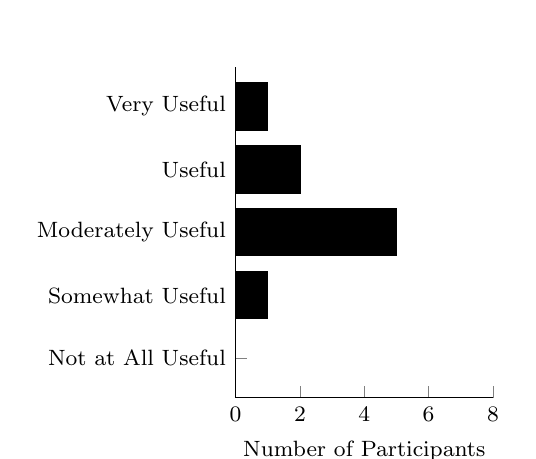
\begin{tikzpicture}
 \begin{axis}[
     xbar stacked,
     ytick=data,
     axis y line*=none,
    axis x line*=bottom,
    tick label style={font=\footnotesize},
    legend style={font=\footnotesize},
    label style={font=\footnotesize},
    xtick={0,2,4,6,8},
    width=.4\textwidth,
    bar width=6mm,
    xlabel= Number of Participants,
    yticklabels={Not at All Useful, Somewhat Useful, Moderately Useful, Useful, Very Useful},
    xmin=0,
    xmax=8,
    area legend,
    y=8mm,
    enlarge y limits={abs=0.625},
]

\addplot[fill=black] coordinates
{(0,0) (1,1) (5,2) (2,3) (1,4)};
\end{axis}  
\end{tikzpicture}
\caption{Survey Results on the Usefulness of \tooltwo}
\label{fig:class-survey}
\end{figure}


\subsubsection{Validation Frequency}

One area of improvement for the \tooltwo system is to improve how students verify their project. Even though we found students started programming assignments significantly earlier when automated issues were present, we also found that students reported waiting until the end of the development process to validate their work met the project expectations. For example, several students noted that, while they they found \tooltwo notifications useful, they ``\textit{didn't really check them until the final day}'' (P1) and ``\textit{checked it once at the end to make sure everything was correct but thats it}'' (P7). Furthermore, P7, who ranked the system the lowest as Somewhat Useful, added ``\textit{I kept track of my own progress so I did not feel the need for this}''. This problem also exists in software engineering where, while research shows validating and verifying software through out the development process improves code quality~\cite{Wallace89Verification}, professional developers often face challenges and delay validating their program meets project requirements~\cite{Garcia08Ten}. This motivates the need for automated recommendations to better integrate into development workflows by encouraging programmers to validate their code more frequently.

\subsubsection{Update Frequency}

Similarly, participants desired more frequent updates from \tooltwo. For example, students mentioned ``\textit{I liked it but would like it more
if it could be updated more often, or maybe later in the day}`` (P1) and ``\textit{the class bot didn't update frequently enough}'' (P2). Additionally, P4 thought the bot was broken due to infrequent updates and then ``\textit{did not trust it when it started to work}''. Prior work in software engineering, including the results of the \tele study, shows that untimely notifications discourage developers from adopting recommendations~\cite{viriyakattiyaporn2009challenges, Sorry}. Furthermore, researchers found presenting static analysis tool output more frequently encouraged programmers to fix more bugs~\cite{Distefano2019Facebook}. While this system incorporated temporal locality into its design by consistently updating GitHub issues, students desired even more frequent feedback and updates from the system to support them in their work. Providing frequent updates to projects can improve the integration of automated recommendations into programmers' workflows and increase the effectiveness of digital nudges for improving the adoption of developer behaviors.

\subsection{Summary}

The results from this study show that that nudges are useful for improving student programming behaviors. Specifically, we found that \tooltwo significantly improved student grades, increased the number of changes to repositories, and encouraged students to start programming earlier. Participants also reported this system was useful and provided insight
for improving automated nudges to encourage better software
engineering behaviors by better incorporating student workflows. We analyzed this feedback and present two themes based on how frequently students checked the automated notifications from \tooltwo and how often the issues were updated.

\section{Discussion}

Ultimately, this work shows incorporating \framework into automated recommendations can improve the behavior and decision-making of developers. To support this, I implemented \tooltwo as a recommender system incorporating the conceptual framework. This system was designed to include each of the choice architecture principles by generating \textit{actionable} GitHub issues with automated updates to recommend development tasks, providing straightforward and visual \textit{feedback} to track progress on projects, and presenting updates with persistent and convenient \textit{locality} on issues in the repository during development. To analyze the impact of this approach on the behavior of programmers, I developed \tooltwo to encourage student programmers to adhere to software engineering processes in their work. 

Research shows adopting software processes is a beneficial developer behavior for improving the quality of applications~\cite{Clark97theeffects}. However, Computer Science education research shows failing to adhere to software engineering processes leads to high failure and attrition in early programming courses~\cite{beaubouef2005high}. Moreover, the adoption problem for this developer behavior translates into industry, where professional software engineers also frequently fail to follow advised development practices and inappropriately allocate the time and effort for completing tasks~\cite{Boehm1984SEEcon}. By encouraging students to follow software engineering processes, we found \tooltwo improved the code quality and developer productivity of students by boosting grades, increasing code contributions, and preventing procrastination. I believe these automated nudges incorporating \framework are a step towards encouraging Computer Science students to adopt useful developer behaviors while working on programming projects, and thus improving the behavior of software engineers.



\chapter{CONCLUSION}
\label{chap-end}


\section{Thesis Statement Revisited}

This dissertation presents research to evaluate and support my thesis statement (Chapter~\ref{chap-thesis}). The thesis of this dissertation is: \\

\thesis \\ \\

To support this claim, my research makes the several contributions to advance knowledge on designing automated recommendations to increase adoption of developer behaviors. First, I conducted a \textit{set of experiments} examining \textit{peer interactions} and the \tele as developer recommendation approaches to determine what makes an effective recommendation to software engineers (Chapter~\ref{chap-peer}). The results from these studies show that user-to-user recommendations are effective because of their ability to foster receptiveness, specifically desire and familiarity, while naive bots are ineffective because of their inability to conform to social context and development workflows.

The preliminary studies motivated the need for new techniques to recommend developer behaviors to programmers as opportunities for peer interactions decline and simple systems such as \toolone generate intrusive and unsuccessful notifications. To improve the effectiveness of automated recommendations, I introduce \framework, a \textit{conceptual framework} for designing effective automated recommendations to developers by applying concepts from nudge theory (Chapter~\ref{chap-framework}). This framework utilizes practical tools for choice architecture~\cite{johnson2012beyond} to obtain principles for creating automated recommendations to improve the environment surrounding developers' decisions, and the formative evaluation shows software engineers preferred actionable suggestions compared to static ones. 

To evaluate \framework, I devised a \textit{set of experiments} analyzing an existing recommender system, \suggs, through the lens of this framework to discover its impact on developer preferences and development activity (Chapter~\ref{chap-suggs}). These evaluations show that developers significantly prefer to receive tool recommendations from systems incorporating \framework than those that don't, and that this framework is useful for recommending a variety of changes and effective for improving development activity and collaboration between developers during reviews. 

Finally, to further assess this framework, I developed a novel \textit{automated recommender system}, \tooltwo, that incorporates \framework principles to generate digital nudges recommending useful developer behaviors to Computer Science students (Chapter~\ref{chap-bot}). The findings show that this bot was able to improve code quality and the productivity of students on their programming assignments by encouraging them to follow software engineering processes, a behavior that is also often ignored by professional developers in industry.

In this work, I use concepts from nudge theory to encourage software engineers to adopt better behaviors. I analyze existing and novel recommendation techniques, define \framework as a method to enhance automated recommendations, investigate how this framework impacts existing recommender systems, and develop a bot to show this approach influences programmer behavior by improving code quality and developer productivity.

\section{Future Work}

This dissertation motivates, presents, and evaluates \framework, a novel framework that incorporates nudge theory to design effective automated recommendations to encourage developer behaviors. Future directions of this research can further enhance automated developer recommendations by \textit{analyzing the behavior} of software engineers and \textit{developing new tools} and techniques to improve the decision-making, behavior, and productivity of programmers in their work.

\subsection{Behavior}

Examples of future studies related to this work involve using \framework to suggest additional developer behaviors, predicting the actions of programmers to proactively make recommendations to prevent bad behaviors, and exploring other disciplines to improve the behavior and decision-making of software engineers.

\begin{itemize}
    \item \textbf{Recommending developer behaviors.} The research presented in this dissertation explores recommendations for several developer behaviors, namely tool adoption (Chapter~\ref{chap-peer}, Chapter~\ref{chap-suggs}.1), code improvements (Chapter~\ref{chap-suggs}.2), and following software engineering processes (Chapter~\ref{chap-bot}). Future directions of this work can examine the following question: how can \framework impact the adoption of other developer behaviors? For example, research shows software engineers often ignore beneficial development practices such as pair programming~\cite{Lui2010}, software dependency updates~\cite{Samim2017AutoPullRequests}, software migration~\cite{SmartSheet}, and more. Future work can explore using the framework presented in this dissertation to design developer recommendations for additional tools and practices.
    
    \item \textbf{Predicting developer behavior.} For the most part, my research is largely reactive in that it makes recommendations to suggest developer behaviors after programmers have completed a programming task inefficiently. To improve the effectiveness of automated recommendations to developers, future work can explore developing proactive nudges to predict the actions of developer and present suggestions before bad behaviors occur. For example, machine learning techniques such as collaborative filtering~\cite{Murphy-Hill2012Fluency} or Bayesian user modeling~\cite{HorvitzLumiere} can be applied to analyze previous development activities of software engineers and anticipate poor decisions in advance. Then, recommender bots can proactively suggest better practices to help developers avoid poor practices and increase adoption of beneficial behaviors.
    
    \item \textbf{Interdisciplinary behavioral concepts.} Nudge theory is a behavioral science concept for improving human decision-making and behavior. To advance this research, future work can explore techniques for modifying human behavior from other disciplines. For example, behavioral science also posits \textit{shoves} as an alternative to nudges that force humans to adopt target behaviors~\cite{Shove}. Likewise, user experience and human factors research submits \textit{dark patterns}, or deceptive user interface designs, as another form of indirect influence to alter user behavior online.\footnote{\url{https://darkpatterns.org/index.html}} Prospective studies can explore multidisciplinary techniques to influence human behavior and apply these concepts to influence the behavior of software engineers.
\end{itemize}

\subsection{Tools}

Potential advancements of this research also include subsequent studies examining using \framework to improve the adoption of systems produced by research in industry, enhance the output of development tools, and creating new bots to encourage the adoption of developer behaviors.

\begin{itemize}
    \item \textbf{Improving research products.} As mentioned in Section 3.1.1, there are a variety of factors that contribute to the developer behavior adoption problem. While the research presented in this dissertation primarily focuses on improving the decision-making of software engineers, future work can investigate ways to improve other barriers to the adoption of development tools and practices. For example, studies show the development products and tools developed by researchers are often ineffective for industry practitioners~\cite{norman2010research,wohlin2013empirical}. Future research can explore ways to bridge the research-practice gap and improve the adoption of developer behaviors by convincing researchers and toolsmiths to develop and evaluate products relevant to software engineers that accommodate developer needs. By doing this, we can increase the awareness of software engineering research, techniques, and findings and adoption of useful tools and practices in industry.
    
    \item \textbf{Tool output.} This dissertation introduces \framework as a framework to design recommendations encouraging developers to adopt code fixes (\suggs) and software engineering processes (\tooltwo) to apply to their work. Another application of this research is to enhance how problems are presented to programmers. Research shows developers often ignore warnings for code smells, or potential problems within code~\cite{Yamashita2013CodeSmells}, and avoid static analysis tools due to incomprehensible output~\cite{Johnson2013Why}. Prior work has also explored ways to improve code smell notifications, including techniques to provide actionable static analysis alerts that mitigate false positives~\cite{Heckman2010Model}, lightweight visualizations to inspect smells during code reviews~\cite{Parnin2008CodeSmells}, ambient interactive designs to support identifying and refactoring code smells~\cite{MurphyHill2010CodeSmells}, and developer-driven code smell prioritization to rank bugs based on criticality~\cite{Pecorelli2020DDCodeSmells}. To reduce code smells and increase the quality of code, future work can build on this research by using \framework to design code smell notifications and nudge developers to fix reported issues and further encourage the adoption of useful tools and practices.

    \item \textbf{Nudge bots.} To further improve the behavior of developers, future work can develop automated tools incorporating \framework principles and concepts from nudge theory to make recommendations using different interventions. For example, this work examines recommendations on GitHub through automated pull requests (Chapter~\ref{chap-peer}.2), \sugg (Chapter~\ref{chap-suggs}), and automated issues (Chapter~\ref{chap-bot}). Future directions of this work can explore delivering recommendations to software engineers through similar techniques on other code hosting websites like GitLab\footnote{\url{https://about.gitlab.com/}} or BitBucket.\footnote{\url{https://bitbucket.org/}} Additionally, future work can recommend developer behaviors to software engineers through mechanisms evaluated in prior work such as StackOverflow posts~\cite{cai2019AnswerBot},\footnote{\url{https://stackoverflow.com/}} instant messages through Slack~\cite{lin2016slack},\footnote{\url{https://slack.com/}} posts to social media~\cite{begel2010social} or blog sites~\cite{barik2015heart},\footnote{\url{https://news.ycombinator.com/}} and other online programming communities. Furthermore, research can also explore other interventions such as chatbots~\cite{cerezo2019building} or automated program repair techniques~\cite{monperrus2019Repairnator} to recommend developer behavior. These examples can provide further methods to incorporate \framework recommendations to encourage the adoption of beneficial behaviors by developers.
\end{itemize}

\section{Epilogue}

\begin{center}
%\begin{quote}
\textit{``I think the most interesting topic for software engineering research in the next ten years is, \\\textbf{`How do we get working programmers to actually adopt better practices?'}}''\footnote{\url{https://twitter.com/gvwilson/status/1142245508464795649?s=20}}
%\end{quote}
\end{center}



%%---------------------------------------------------------------------------%%
%%  Bibliography 

%%  You can use the bibitem list.
%\bibliographystyle{unsrt}
%\begin{%thebibliography}{99}
%\bibitem{cb02}
%Casella, G. and Berger, R.L. (2002)
%\newblock {\it Statistical Inference, Second Edition.}
%Duxbury Press, Belmont, CA.
%
%\bibitem{t06}
%Tsiatis, A.A. (2006)
%\newblock {\it Semiparametric Theory and Missing Data.}
%Springer, New York.
%
%\end{thebibliography}

%% or use BibTeX
%\bibliography{dcbrow10}{}
\bibliographystyle{plain}
%\nociterec{*}

%\bibliographystyle{plainnat}%plainnat is necessary to enable the use of citet. Natbib style file.
%\bibliography{Ortiz-thesis2}
%\ensureoddstart
\begin{spacing}{1}
 \setlength\bibitemsep{11pt} %22pt = 2*11pt, where fontsize is 11pt
 \phantomsection
 \addcontentsline{toc}{chapter}{{\uppercase{\bibname}}} %\textorpdfstring and \uppercase needed due to hyperref package http://www.latex-community.org/forum/viewtopic.php?f=44&t=16601
 %\vspace{-0.5in}
\titleformat{\chapter}[display]{\bf\filcenter
}{\chaptertitlename\ \thechapter}{11pt}{\bf\filcenter}
\titlespacing*{\chapter}{0pt}{0.0in-9pt}{22pt}

\printbibliography[heading=myheading]
\end{spacing}
%\bibliographystyle{apalike}


%%---------------------------------------------------------------------------%%
% Appendices
%\ensureoddstart
\appendix


\renewcommand*{\thefootnote}{\fnsymbol{footnote}}
\setcounter{footnote}{0}
\chapter{Study Materials for Chapter 4}
\label{app-prelim}

%\newcommand{\TODO}[1]{{\color{red}\bfseries [[TODO: #1]]}}
\newcommand{\todo}[1]{{\color{red}\bfseries [[TODO: #1]]}}

\hyphenation{retro-active-ly recommend-ation}

\newcommand\insight[1]{
	\noindent 
	\fcolorbox{gray!20}{gray!20}{
		\parbox{0.92\columnwidth}
		{#1}
		\hspace*{0.5ex}
	}
}

\newcommand{\tooltwo}{\texttt{class-bot}\xspace}
\newcommand{\toolone}{\texttt{tool-recommender-bot}\xspace}

\newcommand{\tele}{naive \textit{telemarketer design}\xspace}
\newcommand{\TELE}{Naive \textit{Telemarketer Design}\xspace}
\newcommand{\suggs}{GitHub \textsl{suggested changes}\xspace}
\newcommand{\sugg}{\textsl{suggested changes}\xspace}
\newcommand{\SUGGS}{GitHub \textsl{Suggested Changes}\xspace}
\newcommand{\suggtag}{\texttt{\`\`\`~\texttt{suggestion}}\xspace}
\newcommand{\fence}{\texttt{\`\`\`}\xspace}
\newcommand{\ep}{\textsc{Error Prone}\xspace}
\newcommand{\EP}{\textsc{Error Prone}\xspace}
\newcommand{\pom}{\textit{pom.xml}\xspace}
\newcommand{\PEP}{\texttt{PEP 3105}\xspace}
\newcommand{\ser}{R}
\newcommand{\see}{C}


\newcommand{\framework}{\textsl{developer recommendation choice architectures}\xspace}
\newcommand{\Framework}{\textsl{Developer recommendation choice architectures}\xspace}
\newcommand{\FrameWork}{\textsl{Developer Recommendation Choice Architectures}\xspace}
\newcommand{\FRAMEWORK}{\textbf{\em developer recommendation choice architectures}\xspace}

\newcommand{\thesis}{\insight{By incorporating \FRAMEWORK into recommendations for software engineers, we can \textbf{\em nudge} developers to adopt behaviors useful for improving code quality and developer productivity.}}


\section{\em ``How Software Users Recommend Tools to Each Other''}
\label{app-peer}

% \subsection{Data}

% The dataset participants analyzed to complete the tasks is available online.\footnote{https://www.kaggle.com/c/titanic/data}

\subsection{Study Script}
\label{app-peer-tasks}

\subsubsection*{\large Pre Task:} 

The dataset is picked from kaggle.com’s Titanic competition: 

\url{https://www.kaggle.com/c/titanic} \\

\noindent
The Variable descriptions are given here: 

\url{https://www.kaggle.com/c/titanic/data} \\

\noindent
Answer any questions about the dataset. \\

\noindent
Please do not use the internet to answer the questions. \\

\noindent
Please work on the tasks together in pairs.   \\

\noindent
The time to spend on the task is 60 mins, which comes to 7 to 8 mins on each task. However, this is just a recommendation. 
(the participants were asked to do their best when answering the questions and not to bother about the time etc. ) \\

\noindent
Please use any tool you are comfortable with to answer these questions. This computer has Excel, Rstudio, Python, SAS JMP Pro 12, and MySQL Workbench. If you need anything else, we can download that as well.  \\

\noindent
\textbf{The total time for the task is 60 mins. Please do not spend more than 45 mins in the training tasks which comes to around 7 to 8 mins on each question.} 

\subsubsection*{\large Tasks:}

\textbf{Student Task}

\noindent
Task: For a to e, please to describe the relationship. For f the factors should be ranked from the most significant to least significant. You can use mean, mode, etc. to explain the ranking. \\

\noindent
\textbf{Using training data: (45 mins)}
\begin{itemize}
    \item[a.] What is the relationship between the (gender, age) and number of sibling/spouse (SibSp) traveling? 
    \item[b.] What is the  relationship between the Title(you can find this in the name) and the number of children/parents (Parch) traveling? 
    \item[c.] What is the relationship between the Title(you can find this in the name) and the age and gender? 
    \item[d.] What is the relationship between (class, fair) and age? 
    \item[e.] What is the relationship between (the fare and class) and the city embarked? 
    \item[f.] Please rank all the factors (a-e) for their contribution to survival. The factors should be ranked from the most significant to least significant. You can use mean, mode, etc. to explain the ranking.
\end{itemize}

\noindent
\textbf{On the testing data: (10 mins)}

Please find whether these people survived.

\begin{itemize}
    \item[a.] Chaffee, Mrs. Herbert Fuller (Carrie Constance Toogood)
    \item[b.] Robins, Mr. Alexander A
    \item[c.] Peltomaki, Mr. Nikolai Johannes 
    \item[d.] Abelseth, Mr. Olaus Jorgensen
    \item[e.] Mulvihill, Miss. Bertha E
    \item[f.] Thomas, Mr. John
    \item[g.] Daniels, Miss. Sarah
    \item[h.] Delalic, Mr. Redjo
\end{itemize}

\noindent
\textbf{LAS Analyst Task}

\noindent
Task: For a to c, please describe the relationship between the categories. For d the factors should be ranked from the most significant to least significant. You can use mean, mode, etc. to explain the ranking. \\

\noindent
\textbf{Using train.csv: (35 mins)}
\begin{itemize}
    \item[a.] What is the relationship between the gender (Sex), age, and the number of siblings/spouse traveling (SibSp)? 
    \item[b.] What is the relationship between the Title (you can find this in the name- Mr., Mrs., Ms., Miss., Master., Dr.,  etc. There may be more than this) and the number of children/parents (Parch) traveling?
    \item[c.] What is the relationship between the fare, class (Pclass), and age? 
    \item[d.] Rank the factors for their contribution to survival. The factors should be ranked from the most significant to least significant. You can use any methods to explain the ranking. (1 = survived, 0 = died)
\end{itemize}
   

When you are comfortable with your answers to the tasks above or time is running out, please move on to the final task. Again, you must work together in pairs and you may not use the internet to answer the questions. \\

\noindent
\textbf{Using test.csv and your results from the previous task: (10 min.)}

Predict whether the following passengers survived:

\begin{itemize}
    \item[a.] Chaffee, Mrs. Herbert Fuller (Carrie Constance Toogood)
    \item[b.] Robins, Mr. Alexander A
    \item[c.] Peltomaki, Mr. Nikolai Johannes 
    \item[d.] Abelseth, Mr. Olaus Jorgensen
    \item[e.] Mulvihill, Miss. Bertha E
    \item[f.] Thomas, Mr. John
    \item[g.] Daniels, Miss. Sarah
    \item[h.] Delalic, Mr. Redjo
\end{itemize}


\subsubsection*{\large Post Task:} 

For the tasks you just completed, I’m interested in when you recommended a tool or program feature to complete the tasks. I noticed the following recommendations you made; let’s look back at them briefly. 
\textit{Open recommendation sheets.}

Do you recall making any other recommendations that I didn't write down, especially ones where help was not specifically asked for? \textit{Write them down.}

Now, let’s go through each one. May I turn on my audio recorder? \textit{Turn it on. Fill in interview portion.}


\subsection{Recommendation Sheet}

The following text was used by the researchers to track instances of peer interactions during the study sessions and to guide the discussion in the semi-structured interviews at the end of the tasks: \\

\noindent
\textbf{\Large Recommendation Sheet} \\

\textbf{Observation Data}

Person making the recommendation:  \_\_\_\_\_\_\_\_\_\_\_\_\_\_\_\_\_\_\_\_\_\_\_

Approximate time recommendation made:  \_\_\_\_\_\_\_\_\_\_\_\_\_\_\_\_\_

Tool recommended \_\_\_\_\_\_\_\_\_\_\_\_\_\_\_\_\_\_\_\_ \\

\subsection{Interview Data}
\label{app-peer-interview}

\noindent
\textbf{Semi-structured}

\noindent
\~One effective and one ineffective tool recommendation

\noindent
Previous experience with tool of choice?

\noindent
For person making the recommendation:

\begin{itemize}
    \item Why did you decide to make this recommendation?
    \item Why did you make it this way? 
    \item Why did you phrase it this way?
    \item Why did you make it at this time?
    \item Did the recomendee react in the way you expected?
    \item Anything else we should know about this?
\end{itemize}

\noindent
For person who received the recommendation:
\begin{itemize}
    \item What did you think when you got the recommendation?
    \item How helpful was the recommendation for the task you were doing? For future tasks?
    \item How helpful was the timing of the recommendation?
    \item How disruptive was the timing of the recommendation?
    \item Anything else we should know about this?
\end{itemize}

\subsection{Interaction Data List}
\label{app-peer-data}

For each recommendation observed in our study, we collected:

\begin{itemize}[topsep=0pt,itemsep=-1ex,partopsep=1ex,parsep=1ex]
    \item the type of peer interaction (Peer Observation or Peer Recommendation),
    \item the approximate time in the video the recommendation took place,
    \item which participants are the driver and navigator,
    \item the study task,
    \item the method of the driver and navigator (if possible),
    \item the name and type of the recommended feature,
    \item a transcript of the dialogue concerning the new tool,
    \item the reaction of the recommendee,
    \item instances in the study where the tool was re-used,
    \item instances where the tool was ignored for a less efficient method,
    \item the effectiveness, politeness, persuasiveness, and receptiveness scores, 
    \item whether the recommendations was under time pressure, and
    \item if the recommendation was discussed during the interview and time of discussion in the video.
\end{itemize}

\subsection{Peer Interaction Characteristic Scoring}
\label{app-peer-scoring}

This section of the appendix presents the final set of criteria that the two independent researchers agreed upon for Politeness, Persuasiveness, and Receptiveness. We specifically searched for the following when analyzing the study videos and scoring these characteristics for peer interactions. \\

\noindent
\textbf{\underline{Politeness}}

\noindent
\textbf{Tact}\\
\textbf{+1} Recommender provides beneficial reason for using tool \\
\textbf{0}  No statement on advantages or disadvantages of tool \\
\textbf{-1} Recommender notes weakness of using suggested tool \\

\noindent
\textbf{Generosity} \\
\textbf{+1} Recommender offers to do the work for the recommendee \\
\textbf{0}  No statement on either peer doing work \\
\textbf{-1} Recommender makes partner complete all the work \\

\noindent
\textbf{Approbation} \\
\textbf{+1} Recommender praises or compliments partner \\
\textbf{0}  No statements of praise or insults \\
\textbf{-1} Recommender insults or offends partner \\

\noindent
\textbf{Modesty} \\
\textbf{+1} Recommender expresses humility in knowledge or abilities\\
\textbf{0}  No statements of humility or arrogance \\
\textbf{-1} Recommender praises their own knowledge or abilities \\

\noindent
\textbf{Agreement}\\
\textbf{+1} Recommender agrees with statements made by partner or uses inclusive language\\
\textbf{0}  No statements of agreement or disagreement\\
\textbf{-1} Recommender disagrees or argues with partner\\

\noindent
\textbf{Sympathy} \\
\textbf{+1} Recommender expresses congratulations, commiseration, or expresses condolences \\
\textbf{ 0}   No statements regarding sympathy or apathy \\
\textbf{-1} Recommender incites conflict, expresses dismissiveness, or enjoys pain of partner \\

\noindent
\textbf{\underline{Persuasiveness}}\\
\noindent
\textbf{Content} \\
\textbf{+1} Recommender explicitly explains why the tool suits the purpose by citing a source, relating to previous experience, explaining how it works, or presenting why it's useful  \\
\textbf{-1} Recommender does not provide any information explaining why to use the suggested tool \\

\noindent
\textbf{Structure} \\
\textbf{+1} Recommender presents the tool before explaining why it should be used \\
\textbf{-1} Recommender explains why a tool should be used before saying the tool or does not provide content \\

\noindent
\textbf{Style}
\textbf{+1} Recommender avoids hedging, hesitating, recommending multiple features simultaneously, asking if a tool should be used, tag questions, and passive and powerless language (i.e. ``I think'', ``I guess'', ``sort of'', excessive number of ``Uh...'', etc.) \\
\textbf{-1} Recommender uses the statements above in their recommendation\\

\noindent
\textbf{\underline{Receptiveness}} \\
\textbf{Demonstrate Desire} \\
\textbf{+1} Recommendee explicitly expresses interest or asks questions to learn more information about tool \\
\textbf{0}  No statements demonstrating desire \\
\textbf{-1} Recommendee explicitly expresses disinterest in using tool \\

\noindent
\textbf{Familiarity}\\
\textbf{+1} Recommendee explicitly expresses familiarity with tool and environment or compares to a familiar tool \\
\textbf{0}  No statements on familiarity \\
\textbf{-1} Recommendee explicitly states they are unfamiliar with the tool or environment \\


\subsection{Demographics Questionnaire}
\label{app-peer-survey}

\begin{enumerate}
    \item Gender: \_\_\_\_\_\_\_\_\_\_\_\_
    \item Occupation: \_\_\_\_\_\_\_\_\_
    \item What is your major (or speciality of highest degree earned)? \_\_\_\_\_\_\_\_\_
    \item How many years have you known your group member? \_\_\_\_\_\_
    How would you describe your relationship with your partner? (Check all that apply)
    \begin{itemize}
        \item[a.] Professional \_\_\_
        \item[b.] Personal \_\_\_
        \item[c.] Academic \_\_\_
        \item[d.] None \_\_\_
    \end{itemize}
    \item What software do you know your partner uses regularly? \\ \_\_\_\_\_\_\_\_\_\_\_\_\_\_\_\_\_\_\_\_\_\_\_\_\_\_\_\_\_\_\_\_\_\_\_\_\_\_\_\_\_\_\_\_\_
    \item Have you and your partner worked together in some capacity in the past? \_\_\_\_\_\_\_\_\_\_\_\_\_\_\_\_\_\_
    \begin{itemize}
        \item[a.] If Yes, please describe any computer-based work you have done together: \\
        \_\_\_\_\_\_\_\_\_\_\_\_\_\_\_\_\_\_\_\_\_\_\_\_\_\_\_\_\_\_\_\_\_\_\_\_\_\_\_\_\_\_\_\_\_
    \end{itemize}
    \item How many years of experience do you have with the software(s) your group used to complete the tasks? \_\_\_\_\_\_\_\_\_\_\_\_\_\_\_\_\_\_\_\_\_\_\_\_\_\_\_\_\_\_\_\_\_\_\_\_\_\_\_\_\_\_\_\_\_
\end{enumerate}

\subsection{Participants}
\label{app-peer-participants}

\begin{table}[H]
	\caption{Peer Interaction Study Participants}
	\centering
	\begin{tabular}{lll}
		\hline
		\textbf{Participant} & \textbf{Gender} & \textbf{Major} \\
		\hline
		S1 & Male & Industrial Engineering $   $ $\blacklozenge$\\
		S2 & Male & Computer Science $   $ $\blacklozenge$\\
		%\hline
		S3 & Male & Computer Science $   $ $\blacklozenge$\\
		S4 & Male & Computer Science $   $ $\blacklozenge$\\
		%\hline
		S5 & Male & Computer Science $   $ $\blacklozenge$\\
		S6 & Male & Computer Science $   $ $\blacklozenge$\\
		%\hline
		S7 & Male & Computer Science $   $ $\blacklozenge$\\
		S8 & Male & Computer Science $   $ $\blacklozenge$\\
		%\hline
		S9 & Male & Industrial Engineering $   $ $\blacklozenge$\\
		S10 & Female & Computer Science $   $ $\blacklozenge$\\
		%\hline
		S11 & Female & Biochemistry $   $ $\blacklozenge$\\
		S12 & Female & Biochemistry $   $ $\lozenge$\\
		%\hline
		S13 & Female&Computer Science$   $ $\blacklozenge$\\
		S14 & Male & Computer Science $   $ $\blacklozenge$\\
		\hline \\
		\end{tabular}
	
		\begin{tabular}{lll}
		\hline 
		\textbf{Participant} & \textbf{Gender} & \textbf{Position} \\
		\hline
		L1 & Female & Researcher 
\includegraphics[height=1em]{Chapter-3/images/hands.png} \\
		L2 & Female & Researcher 
\includegraphics[height=1em]{Chapter-3/images/hands.png} \\
		%\hline
		L3 & Male & Program Manager 
\includegraphics[height=1em]{Chapter-3/images/hands.png} 
\includegraphics[height=1em]{Chapter-3/images/computer.png} \\
		L4 &Female&Director of Operations 
\includegraphics[height=1em]{Chapter-3/images/hands.png} 
\includegraphics[height=1em]{Chapter-3/images/computer.png} \\
		%\hline
		L5 & Male &Researcher, Analyst \\
		L6 & Male & Computer Engineer \\
		%\hline
		L7 & Female & Researcher \\ 
		L8 & Male & Language Analyst \\
		%\hline
		L9 & Female & Engineer 
\includegraphics[height=1em]{Chapter-3/images/hands.png} 
\includegraphics[height=1em]{Chapter-3/images/computer.png} \\
		L10 & Female & Engineer 
\includegraphics[height=1em]{Chapter-3/images/hands.png} 
\includegraphics[height=1em]{Chapter-3/images/computer.png} \\
		%\hline
		L11 & Female & Intel Analyst, Researcher 
\includegraphics[height=1em]{Chapter-3/images/hands.png} \\
		L12 & Male & Systems Researcher 
\includegraphics[height=1em]{Chapter-3/images/hands.png} \\
	\hline
	\end{tabular}
    {\footnotesize
	\begin{itemize}[topsep=0pt,itemsep=-1ex,partopsep=1ex,parsep=1ex]
	\centering
        \item[] $\blacklozenge$ Graduate Student $     $ $\lozenge$ Undergraduate Student
        \item[] 
\includegraphics[height=1em]{Chapter-3/images/hands.png} Previous relationship with partner 
        \item[] 
\includegraphics[height=1em]{Chapter-3/images/computer.png} Previously completed computer-based work with partner
    \end{itemize}
    }
	\label{tab:peer-participants}
\end{table}

\newpage

\section{\em ``Sorry to Bother You: Designing Bots for Effective Recommendations''}

\subsection{Naive Telemarketer Design}
\label{app-sorry}

\begin{figure}[H]
  \centering
  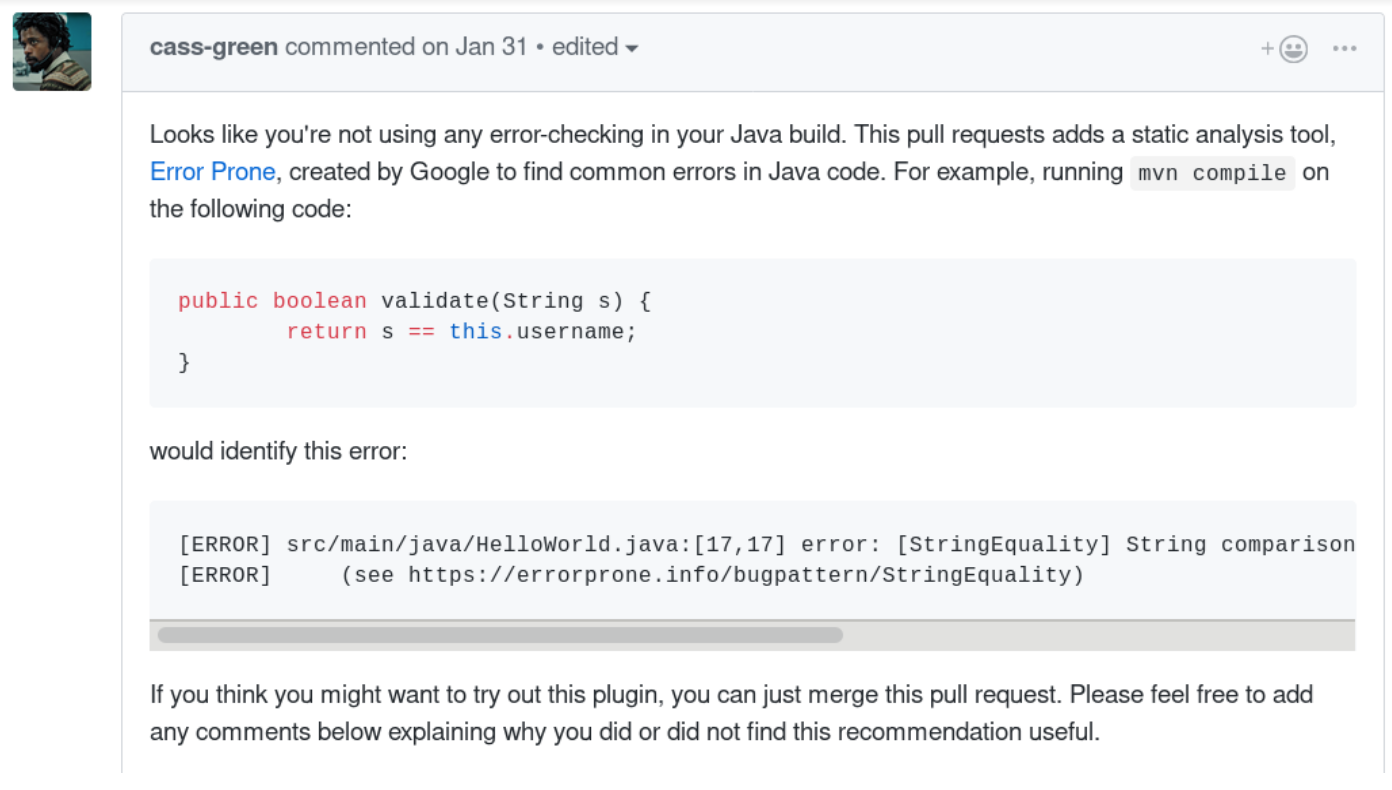
\includegraphics[width=\textwidth]{Appendix-A/images/tele.png}
  \caption{\TELE recommendation from \texttt{tool-recommender-bot}}
  \label{fig:telemarketer}
\end{figure}

\subsection{Study Projects}
\label{app-sorry-projects}

This section outlines the projects that received recommendations for the \tele study and provides the automated pull requests submitted to projects by \toolone:

\begin{enumerate}[topsep=0pt,itemsep=-1ex,partopsep=1ex,parsep=1ex]

\item \url{https://github.com/jponge/lzma-java/pull/15}
\item \url{https://github.com/fizzed/rocker/pull/102}
\item \url{https://github.com/GideonLeGrange/mikrotik-java/pull/61}
\item \url{https://github.com/Asquera/elasticsearch-http-basic/pull/70}
\item \url{https://github.com/debezium/debezium/pull/760}	
\item \url{https://github.com/dropwizard/dropwizard-elasticsearch/pull/34}
\item \url{https://github.com/Nodeclipse/nodeclipse-1/pull/229}	
\item \url{https://github.com/forge/roaster/pull/101}	
\item \url{https://github.com/recommenders/rival/pull/131}{recommenders/rival\#131}
\item \url{https://github.com/tbroyer/gwt-maven-archetypes/pull/58}
\item \url{https://github.com/Hygieia/Hygieia/pull/2696}\footnote[2]{Merged}
\item \url{https://github.com/wro4j/wro4j/pull/1069}\footnote[8]{Merged, then reverted}
\item \url{https://github.com/jplag/jplag/pull/61}
\item \url{https://github.com/gitbucket/markedj/pull/21}	
\item \url{https://github.com/jhalterman/expiringmap/pull/60}		
\item \url{https://github.com/arquillian/arquillian-core/pull/190}
\item \url{https://github.com/graphstream/gs-core/pull/305}
\item \url{https://github.com/jirutka/validator-collection/pull/27}
\item \url{https://github.com/jreijn/spring-comparing-template-engines/pull/37}
\item \url{https://github.com/elkan1788/mpsdk4j/pull/8}		
\item \url{https://github.com/arturmkrtchyan/iban4j/pull/59}	
\item \url{https://github.com/games647/LagMonitor/pull/51}	
\item \url{https://github.com/jmxtrans/jmxtrans-agent/pull/137}	
\item \url{https://github.com/fakereplace/fakereplace/pull/34}		
\item \url{https://github.com/google/binnavi/pull/113}	
\item \url{https://github.com/devnied/AndroidBitmapTransform/pull/1}
\item \url{https://github.com/ebnew/ki4so/pull/7}	
\item \url{https://github.com/bujiio/buji-pac4j/pull/83}	
\item \url{https://github.com/cathive/fx-guice/pull/26}	
\item \url{https://github.com/vvakame/JsonPullParser/pull/43}		
\item \url{https://github.com/cderoove/damp.ekeko/pull/2}	
\item \url{https://github.com/write2munish/Akka-Essentials/pull/8}
\item \url{https://github.com/Slim3/slim3/pull/30}
\item \url{https://github.com/jirutka/spring-rest-exception-handler/pull/30}
\item \url{https://github.com/yyuu/jetty-nosql-memcached/pull/35}
\item \url{https://github.com/casidiablo/persistence/pull/17}	
\item \url{https://github.com/dsyer/sparklr-boot/pull/6}	
\item \url{https://github.com/dgageot/simplelenium/pull/26}	
\item \url{https://github.com/jhalterman/concurrentunit/pull/22}	
\item \url{https://github.com/jplag/jplag/pull/62}
\item \url{https://github.com/kwart/jd-cmd/pull/19}	
\item \url{https://github.com/leveluplunch/levelup-java-examples/pull/5}
\item \url{https://github.com/ngageoint/elasticgeo/pull/97}		
\item \url{https://github.com/perfectsense/dari/pull/317}		
\item \url{https://github.com/rchodava/datamill/pull/119}		
\item \url{https://github.com/RichardWarburton/lambda-behave/pull/98}
\item \url{https://github.com/roundrop/facebook4j/pull/122}	
\item \url{https://github.com/spring-guides/tut-spring-boot-oauth2/pull/97}
\item \url{https://github.com/twitter/hbc/pull/195}	
\item \url{https://github.com/viritin/viritin/pull/362}	
\item \url{https://github.com/SINTEF-9012/JArduino/pull/82}		
\item \url{https://github.com/apache/bigtop/pull/461}
\end{enumerate}
\chapter{Study Materials for Chapter 5}

\section{\em ``Sorry to Bother You Again: Developer Recommendation Choice Architectures for Designing Effective Bots''}

%\subsection{Actionable Recommendations Survey}


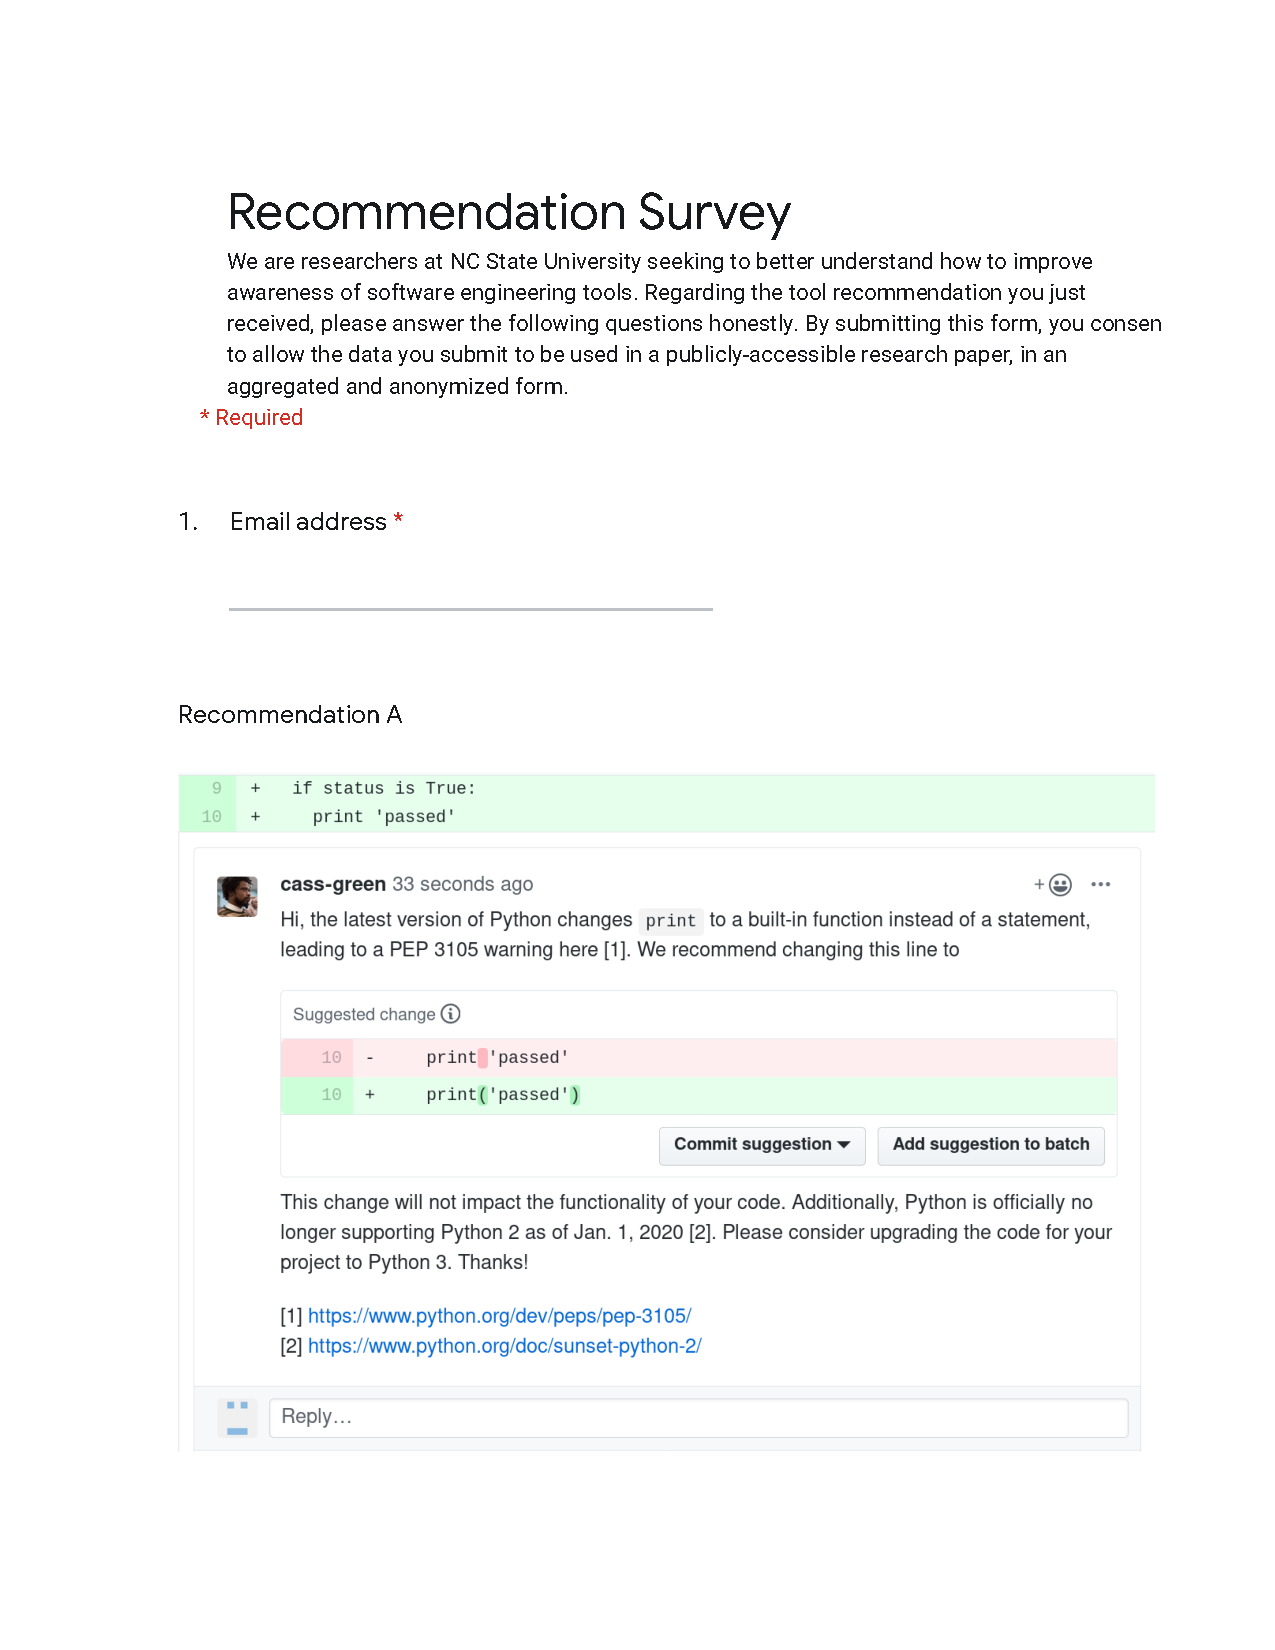
\includepdf[pages=1,pagecommand={\subsection{Actionable Recommendations Survey}\label{app-sorry2-survey}
,\thispagestyle{plain}},scale=.75]{Appendix-B/files/survey.pdf}
\includepdf[pages=2-,pagecommand={\thispagestyle{plain}},scale=.75]{Appendix-B/files/survey.pdf}


\chapter{Study Materials for Chapter 6}
\label{app-suggs}

\section{\em ``Comparing Different Developer Behavior Recommendation Styles''}

\subsection{Recommendation Styles}
\label{app-suggs-recs}
\subsubsection{Email Recommendation}

\begin{figure}[H]
\centering
	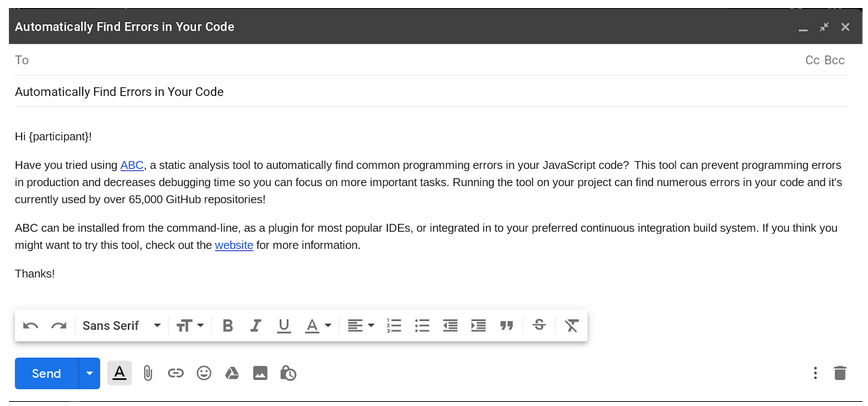
\includegraphics[width=\textwidth]{Appendix-C/images/email-rec.png}
	\caption{Example email recommendation style}	
	\label{fig:email-rec} 
\end{figure}

%Figure~\ref{fig:email-rec}


\subsubsection{GitHub Issue Recommendation}


\begin{figure}[H]
\centering
	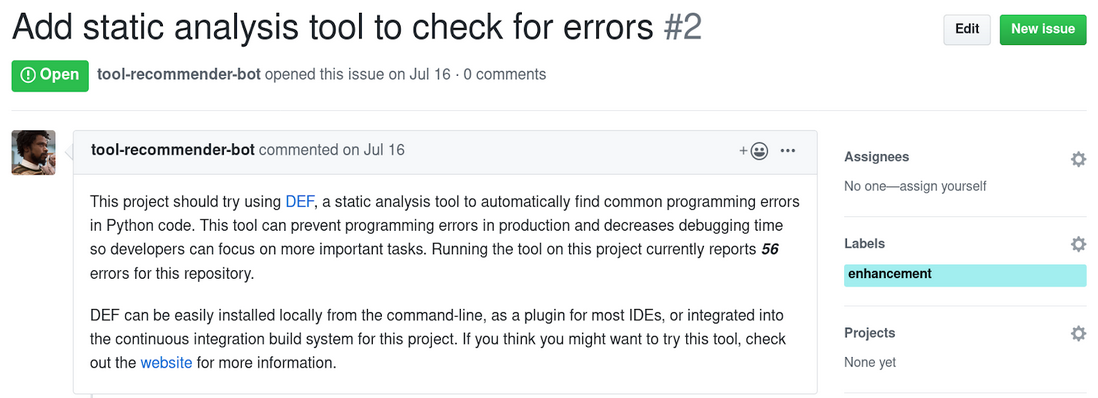
\includegraphics[width=\textwidth]{Appendix-C/images/issue-rec.png}
	\caption{Example GitHub issue recommendation style}	
	\label{fig:issue-rec} 
\end{figure}
%Figure~\ref{fig:issue-rec}

\subsubsection{GitHub Pull Request Recommendation}

\begin{figure}[H]
\centering
	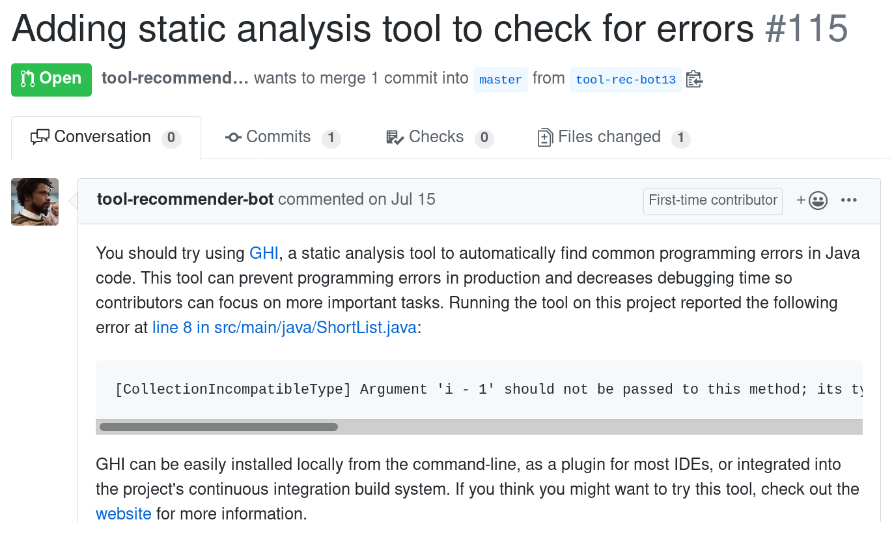
\includegraphics[width=\textwidth]{Appendix-C/images/pull-rec.png}
	\caption{Example GitHub pull request recommendation style}	
	\label{fig:pull-rec} 
\end{figure}

\subsubsection{GitHub Suggested Change Recommendation}

\begin{figure}[H]
\centering
	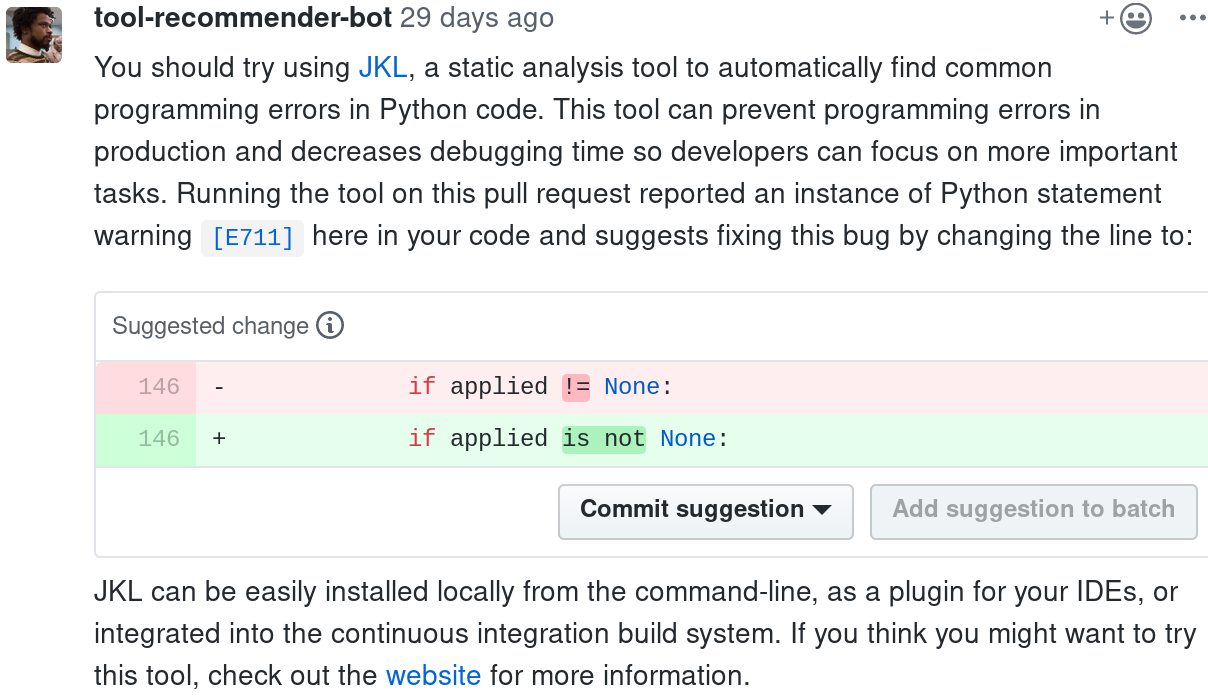
\includegraphics[width=\textwidth]{Chapter-5/images/sugg-recommendation.png}
	\caption{Example \suggs recommendation style}	
	\label{fig:sugg-rec} 
\end{figure}

\newpage

\section{\em ``Understanding the Impact of GitHub Suggested Changes on Recommendations Between Developers''}

\subsection{Suggested Changes Random Sample}
\label{app-suggs-sample}

The following instances of \suggs were randomly sampled from the most recently updated pull requests on repositories and analyzed by researchers to categorize types of recommendations developers make using this feature:

{\footnotesize
\begin{enumerate}[topsep=0pt,itemsep=-1ex,partopsep=1ex,parsep=1ex]
     \item \url{https://github.com/4ian/GDevelop/pull/1112\#discussion_r304598490}
    \item \url{https://github.com/alphagov/govuk-design-system/pull/994\#discussion_r307695226}
    \item \url{https://github.com/angular/angular/pull/31609\#discussion_r308959135}
    \item \url{https://github.com/ansible/ansible/pull/60271\#discussion_r312957415}
    \item \url{https://github.com/apache/cordova-android/pull/764\#discussion_r304199473}
    \item \url{https://github.com/apache/couchdb-documentation/pull/385\#discussion_r251147343}
    \item \url{https://github.com/aragon/aragon-apps/pull/929\#discussion_r308151240}
    \item \url{https://github.com/arXiv/arxiv-search/pull/249\#discussion_r310682583}
    \item \url{https://github.com/aspnet/AspNetCore/pull/10406\#discussion_r286161965}
    \item \url{https://github.com/bbc/simorgh/pull/3048\#discussion_r312518076}
    \item \url{https://github.com/bitcoin/bitcoin/pull/16578\#discussion_r312712522}
    \item \url{https://github.com/BlueBrain/spack/pull/465\#discussion_r309184444}
    \item \url{https://github.com/CasperLabs/CasperLabs/pull/925\#discussion_r313281322}
    \item \url{https://github.com/ceph/ceph/pull/29378\#discussion_r309036721}
    \item \url{https://github.com/chainer/chainerrl/pull/436\#discussion_r299015299}
    \item \url{https://github.com/cosmos/cosmos-sdk/pull/4514\#discussion_r311556341}
    \item \url{https://github.com/cri-o/ocicni/pull/51\#discussion_r311892555}
    \item \url{https://github.com/DataDog/integrations-extras/pull/466\#discussion_r305978895}
    \item \url{https://github.com/dealii/dealii/pull/8384\#discussion_r303584690}
    \item \url{https://github.com/django/django/pull/8119\#discussion_r312538500}
    \item \url{https://github.com/dlang/druntime/pull/2662\#discussion_r300630178}
    \item \url{https://github.com/dotnet/corefx/pull/39917\#discussion_r311788312}
    \item \url{https://github.com/dotnet/dotnet-api-docs/pull/2968\#discussion_r312193646}
    \item \url{https://github.com/elastic/apm-agent-nodejs/pull/1144\#discussion_r309565403}
    \item \url{https://github.com/elastic/kibana/pull/41588\#discussion_r311091394}
    \item \url{https://github.com/ethereum/eth2.0-specs/pull/1361\#discussion_r314107368}
    \item \url{https://github.com/freeCodeCamp/freeCodeCamp/pull/35560\#discussion_r287490144}
    \item \url{https://github.com/galaxyproject/galaxy/pull/8452\#discussion_r313373019}
    \item \url{https://github.com/galaxyproject/tools-iuc/pull/2444\#discussion_r304336637}
    \item \url{https://github.com/gardener/gardener/pull/1128\#discussion_r300451126}
    \item \url{https://github.com/gatsbyjs/gatsby/pull/13471\#discussion_r277948539}
    \item \url{https://github.com/golang/protobuf/pull/785\#discussion_r249270350}
    \item \url{https://github.com/graphql-python/graphene/pull/992\#discussion_r290376085}
    \item \url{https://github.com/greenelab/text_mined_hetnet_manuscript/pull/24\#discussion_r310587566}
    \item \url{https://github.com/HumanCellAtlas/dcp-community/pull/92\#discussion_r310355937}
    \item \url{https://github.com/hyphacoop/handbook/pull/10\#discussion_r303095279}
    \item \url{https://github.com/hyrise/hyrise/pull/1493\#discussion_r258051465}
    \item \url{https://github.com/iterative/dvc/pull/2256\#discussion_r302868825}
    \item \url{https://github.com/jenkinsci/github-branch-source-plugin/pull/235\#discussion_r303663151}
    \item \url{https://github.com/jpmorganchase/quorum/pull/715\#discussion_r286201830}
    \item \url{https://github.com/keybase/client/pull/18045\#discussion_r305071747}
    \item \url{https://github.com/knative/serving/pull/5042\#discussion_r310395773}
    \item \url{https://github.com/Kotlin/KEEP/pull/87\#discussion_r276477734}
    \item \url{https://github.com/kubernetes-sigs/cluster-api/pull/1228\#discussion_r311095643}
    \item \url{https://github.com/kubernetes/kubernetes/pull/79641\#discussion_r313118736}
    \item \url{https://github.com/kubernetes/test-infra/pull/13677\#discussion_r309433430}
    \item \url{https://github.com/LMMS/lmms/pull/4973\#discussion_r287565903}
    \item \url{https://github.com/magento/magento2/pull/22156/\#discussion_r272134087}
    \item \url{https://github.com/mdn/browser-compat-data/pull/4558\#discussion_r309696300}
    \item \url{https://github.com/microsoft/qsharp-compiler/pull/52\#discussion_r311190580}
    \item \url{https://github.com/microsoft/QuantumKatas/pull/111\#discussion_r280869695}
    \item \url{https://github.com/microsoft/terminal/pull/1258\#discussion_r293932790}
    \item \url{https://github.com/mne-tools/mne-python/pull/6233\#discussion_r284656692}
    \item \url{https://github.com/moby/moby/pull/38777\#discussion_r259334795}
    \item \url{https://github.com/neovim/neovim/pull/10071\#discussion_r309415338}
    \item \url{https://github.com/nhsconnect/integration-adaptors/pull/44\#discussion_r310155461}
    \item \url{https://github.com/nistats/nistats/pull/352\#discussion_r313598729}
    \item \url{https://github.com/NixOS/nixpkgs/pull/65724\#discussion_r309807069}
    \item \url{https://github.com/numba/numba/pull/4204\#discussion_r310598073}
    \item \url{https://github.com/numpy/numpy/pull/14197\#discussion_r315005011}
    \item \url{https://github.com/ombulabs/blog/pull/194\#discussion_r310756845}
    \item \url{https://github.com/onnx/onnx/pull/2106\#discussion_r313733168}
    \item \url{https://github.com/open-telemetry/opentelemetry-python/pull/78\#discussion_r314418832}
    \item \url{https://github.com/openhab/openhab2-addons/pull/4664\#discussion_r268409815}
    \item \url{https://github.com/OpenRA/OpenRA/pull/15813\#discussion_r298209839}
    \item \url{https://github.com/operator-framework/operator-sdk/pull/1533\#discussion_r293002730}
    \item \url{https://github.com/ppy/osu-wiki/pull/2419\#discussion_r312936003}
    \item \url{https://github.com/PrismJS/prism/pull/2012\#discussion_r310671629}
    \item \url{https://github.com/publiclab/mapknitter/pull/306\#discussion_r251212108}
    \item \url{https://github.com/pypa/pip/pull/6377\#discussion_r274394104}
    \item \url{https://github.com/Qiskit/qiskit-terra/pull/2650\#discussion_r295429688}
    \item \url{https://github.com/RocketChat/Rocket.Chat/pull/12174\#discussion_r302773285}
    \item \url{https://github.com/rust-lang-nursery/reference/pull/635\#discussion_r302287965}
    \item \url{https://github.com/rust-lang/rust/pull/61708\#discussion_r306056531}
    \item \url{https://github.com/FluidityProject/fluidity/pull/190\#discussion_r309586309}
    \item \url{https://github.com/scikit-learn-contrib/scikit-learn-extra/pull/13\#discussion_r307204657}
    \item \url{https://github.com/scrapy/scrapy/pull/3862\#discussion_r302711618}
    \item \url{https://github.com/security-force-monitor/sfm-cms/pull/585\#discussion_r312087662}
    \item \url{https://github.com/Semmle/ql/pull/1725\#discussion_r314333239}
    \item \url{https://github.com/shopsys/shopsys/pull/1228\#discussion_r310062868}
    \item \url{https://github.com/sipa/bips/pull/52\#discussion_r310589709}
    \item \url{https://github.com/Skyscanner/full-stack-recruitment-test/pull/28\#discussion_r312427118}
    \item \url{https://github.com/sourcegraph/sourcegraph/pull/5062\#discussion_r310050346}
    \item \url{https://github.com/spacetelescope/synphot_refactor/pull/204\#discussion_r307013162}
    \item \url{https://github.com/swcarpentry/git-novice/pull/678\#discussion_r311232763}
    \item \url{https://github.com/syl20bnr/spacemacs/pull/12463\#discussion_r305982291}
    \item \url{https://github.com/sympy/sympy/pull/17266\#discussion_r307727949}
    \item \url{https://github.com/teamleadercrm/api/pull/361\#discussion_r281559715}
    \item \url{https://github.com/tensorflow/community/pull/113\#discussion_r314548430}
    \item \url{https://github.com/terraform-providers/terraform-provider-aws/pull/8916\#discussion_r295438718}
    \item \url{https://github.com/theforeman/smart-proxy/pull/657\#discussion_r292927976}
    \item \url{https://github.com/tombuildsstuff/golang-iis/pull/7\#discussion_r314976753}
    \item \url{https://github.com/vuejs/rfcs/pull/42\#discussion_r296097849}
    \item \url{https://github.com/weaveworks/eksctl/pull/1132\#discussion_r313804187}
    \item \url{https://github.com/WordPress/gutenberg/pull/16873\#discussion_r310070193}
    \item \url{https://github.com/XanaduAI/pennylane/pull/200\#discussion_r288290349}
    \item \url{https://github.com/Zarel/Pokemon-Showdown/pull/5688\#discussion_r312716995}
    \item \url{https://github.com/zeit/next.js/pull/7696\#discussion_r302333269}
    \item \url{https://github.com/zio/zio/pull/1387\#discussion_r314954640}
    \item \url{https://github.com/zkSNACKs/WalletWasabi/pull/2100\#discussion_r313333844}
\end{enumerate}
}



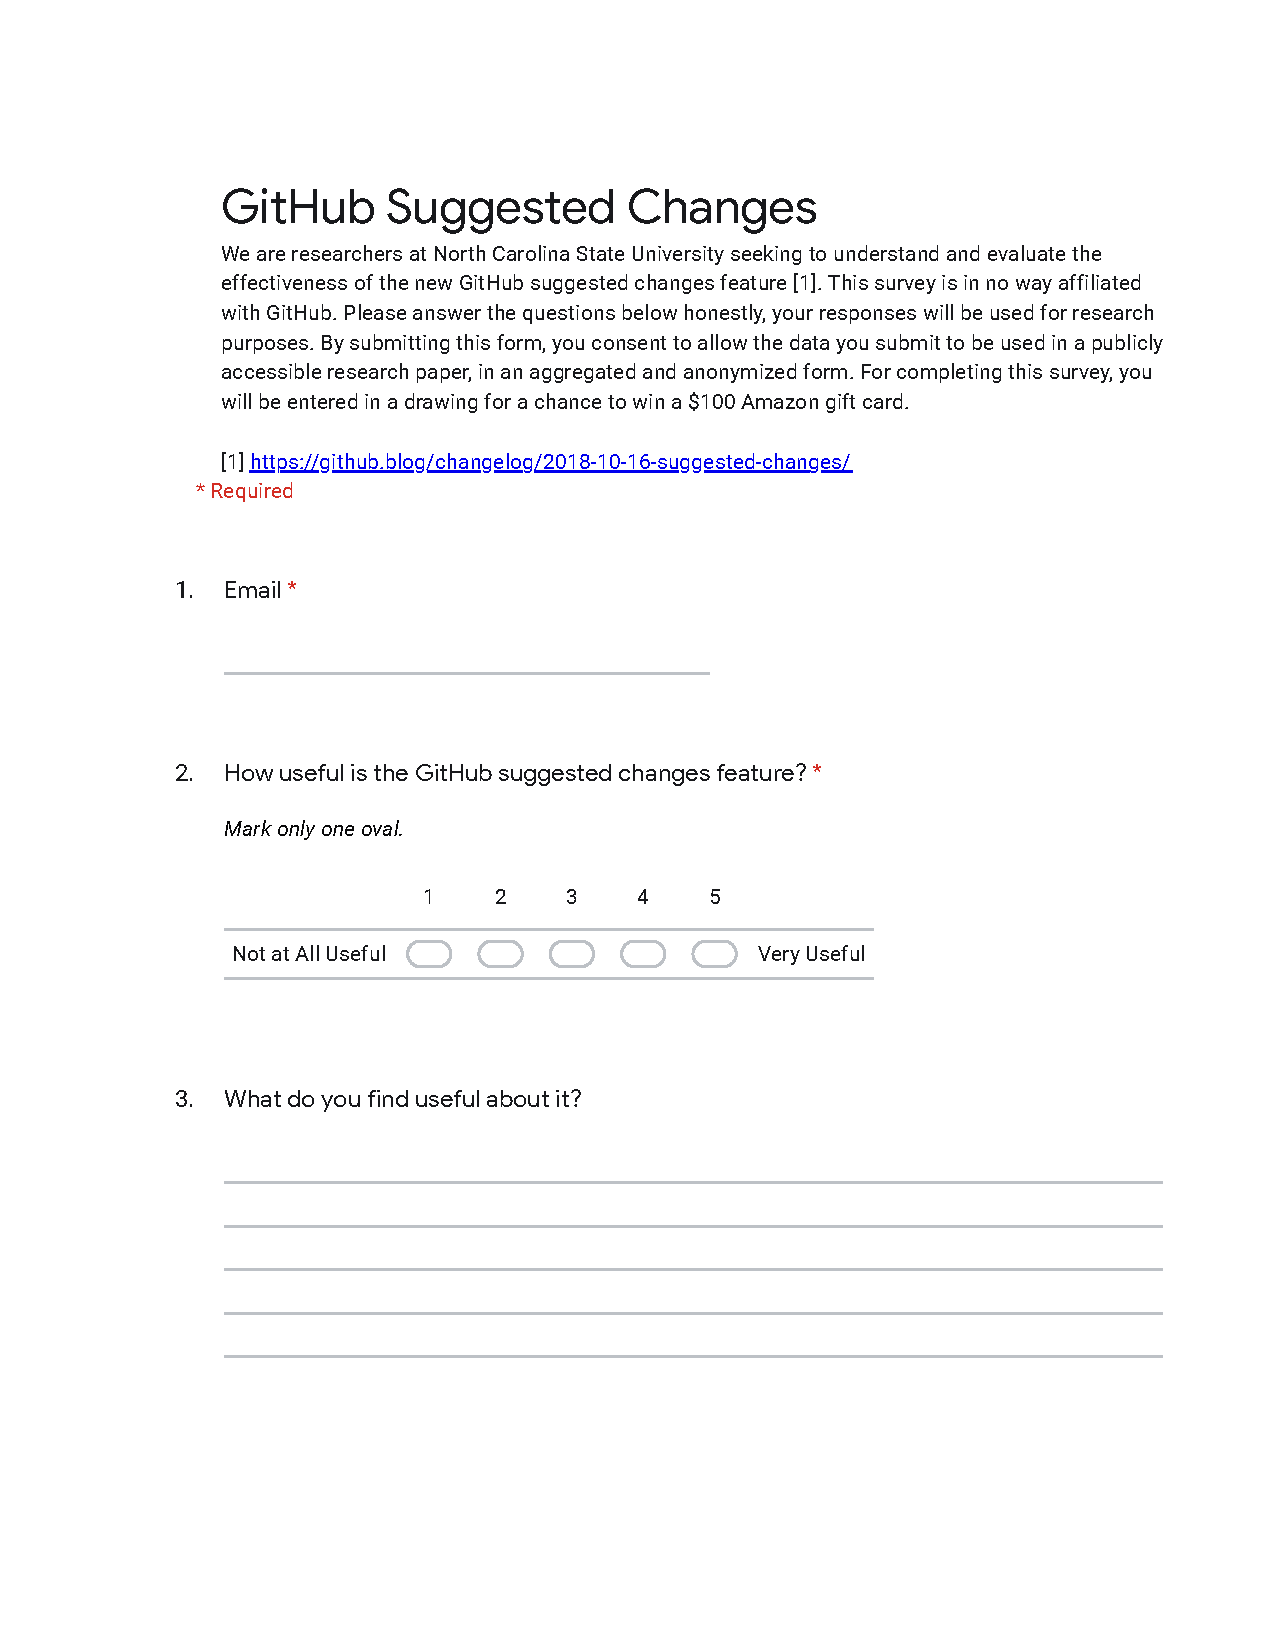
\includepdf[pages=1,pagecommand={\subsection{Suggestee Survey},\thispagestyle{plain}},scale=.75]{Appendix-C/files/suggestee.pdf}
\includepdf[pages=2-,pagecommand={\thispagestyle{plain}},scale=.75]{Appendix-C/files/suggestee.pdf}

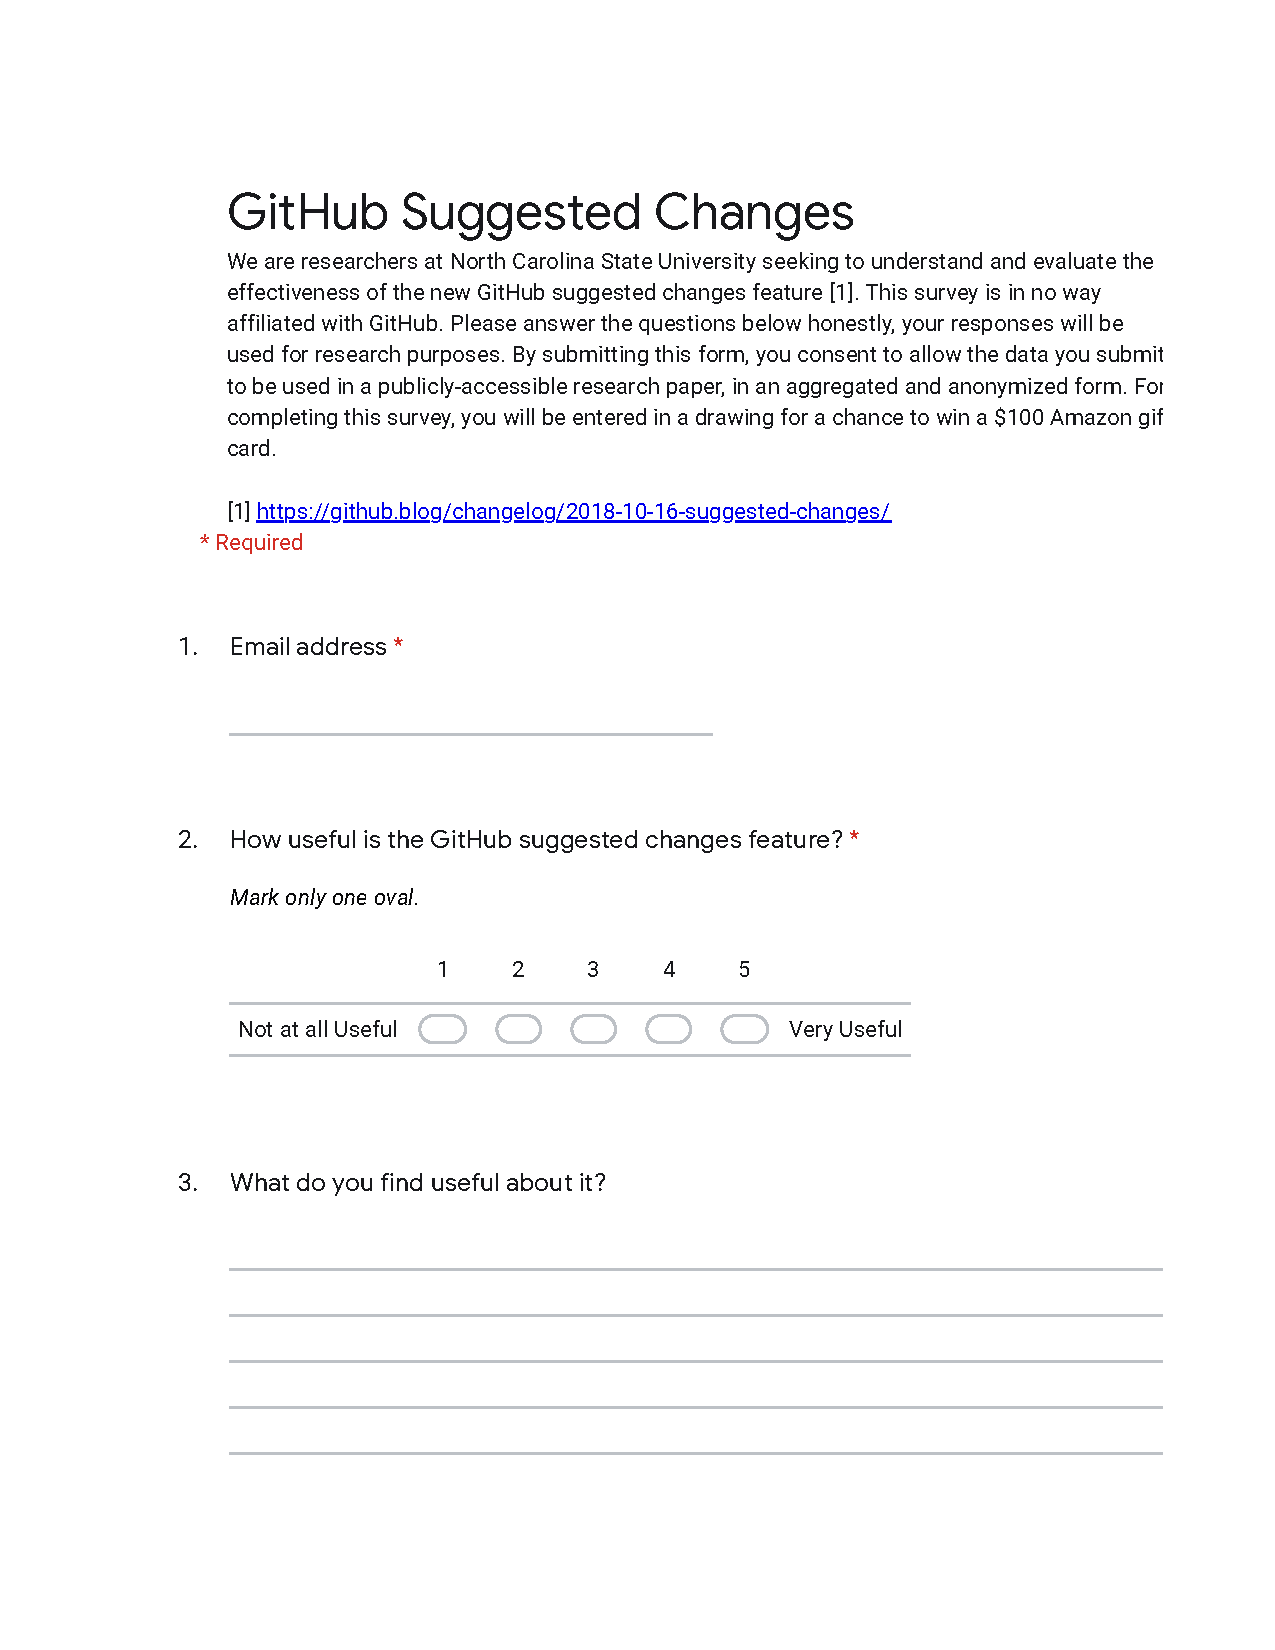
\includepdf[pages=1,pagecommand={\subsection{Suggester Survey},\thispagestyle{plain}},scale=.75]{Appendix-C/files/suggester.pdf}
\includepdf[pages=2-,pagecommand={\thispagestyle{plain}},scale=.75]{Appendix-C/files/suggester.pdf}
\chapter{Study Materials for Chapter 7}
\label{app-bot}

\section{\em ``Nudging Students Toward Better Software Engineering Behaviors''}

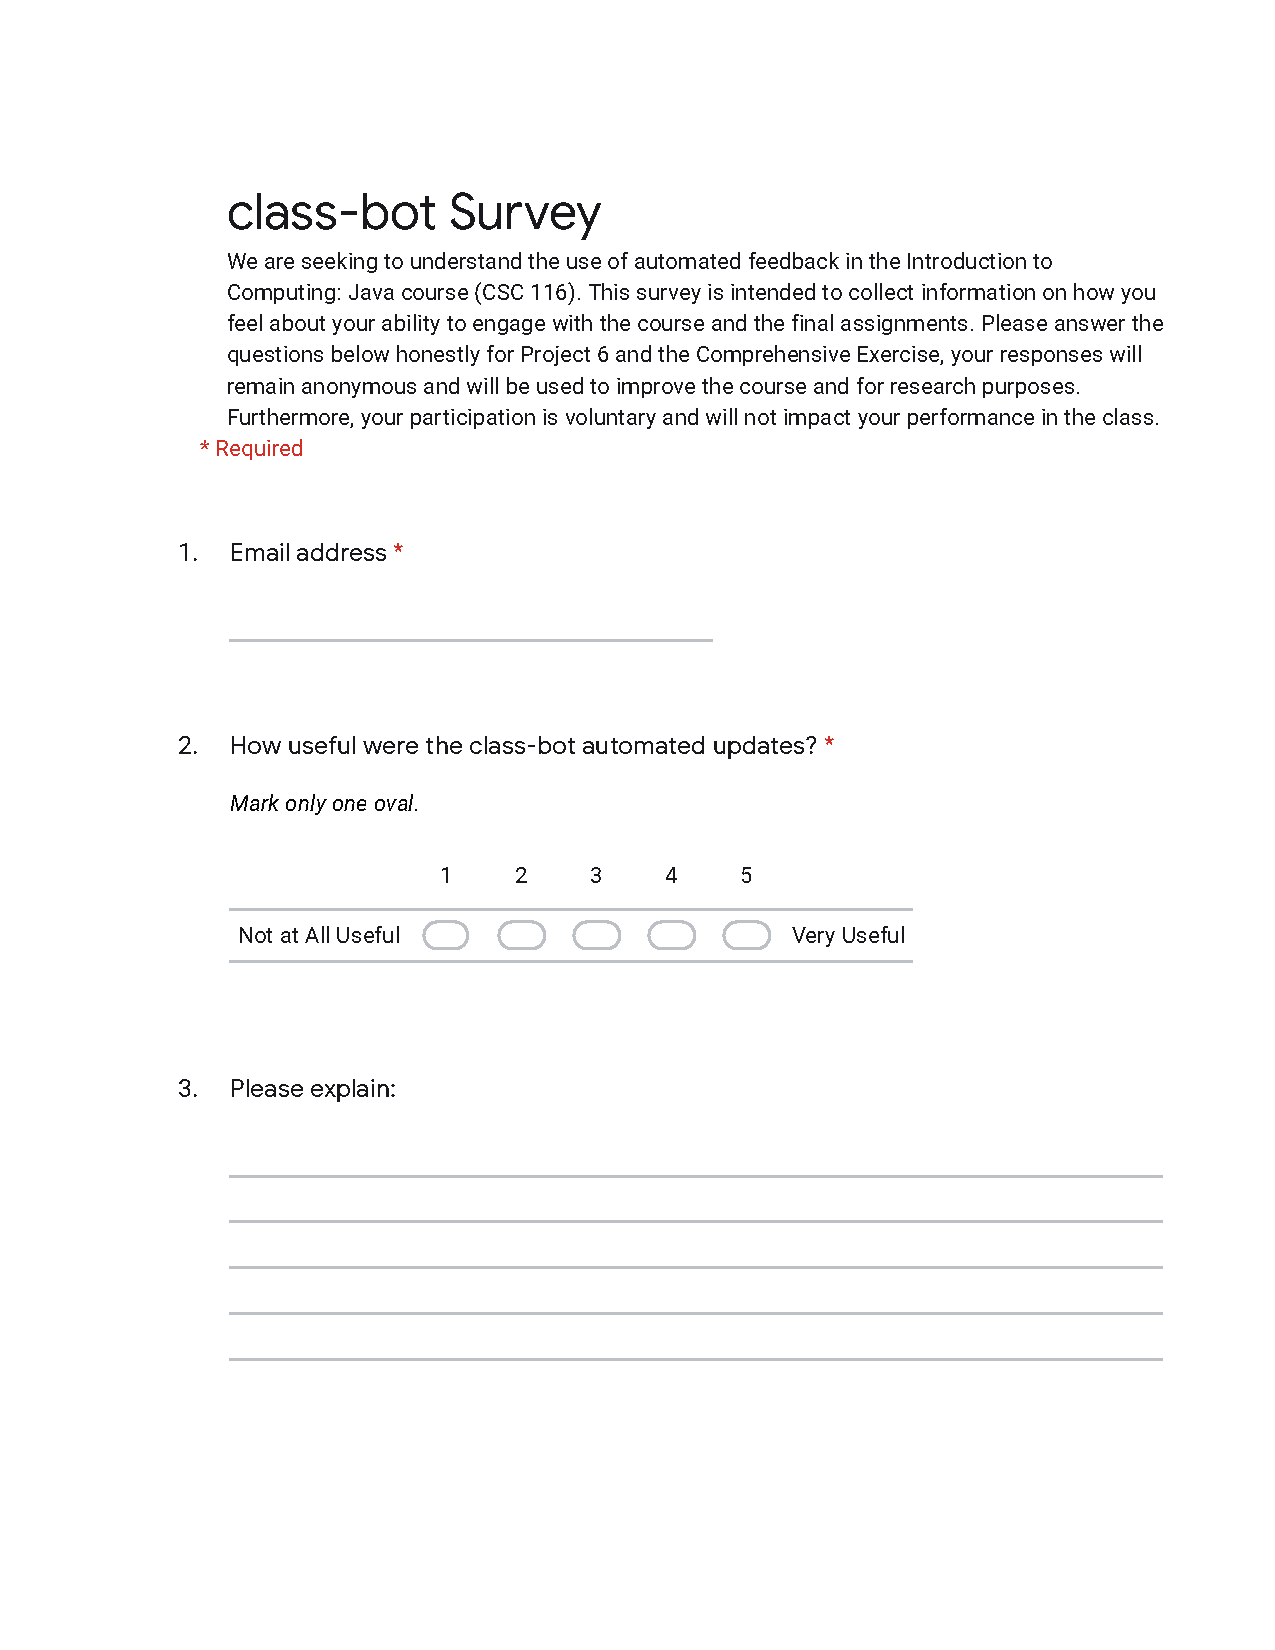
\includepdf[pages=1,pagecommand={\subsection{Survey},\thispagestyle{plain}},scale=.75]{Appendix-D/files/student-survey.pdf}
\includepdf[pages=2-,pagecommand={\thispagestyle{plain}},scale=.75]{Appendix-D/files/student-survey.pdf}

%%---------------------------------------------------------------------------%%
%\ensureoddstart
\backmatter


\end{document}